%!TEX root = ../thesis.tex
%*******************************************************************************
%****************************** Third Chapter **********************************
%*******************************************************************************
\chapter{Data and analysis}

% **************************** Define Graphics Path **************************
\ifpdf
    \graphicspath{{Chapter3/Figs/Raster/}{Chapter3/Figs/PDF/}{Chapter3/Figs/}}
\else
    \graphicspath{{Chapter3/Figs/Vector/}{Chapter3/Figs/}}
\fi

\section[SEM Data]{SEM Data}
\label{section3.1}

\subsection[Azurite and blue verditer]{Azurite and blue verditer}
\label{subsection3.1.1}

This section discusses qualitatively the morphological features, regularity, and approximate particle size of the reference samples described in \textit{Table \ref{table:ref_sample}}.  
% ************************************************     HKI nat az sample     *******************************************************************

\textit{Figures \ref{fig:hki_nat_az_sem_1}-\ref{fig:hki_nat_az_sem_5}} show the sample HKI natural azurite. This sample is of unknown date and provenance but is confirmed to be naturally produced, which offers a baseline against which to compare other samples known to be synthetic or of unknown origin. Maginification ranges from 250x to 4000x. Significant surface charging was not observed with this sample.

In \textit{Figure \ref{fig:hki_nat_az_sem_1}}, two areas are shown at 250x magnification. Particle sizes are very irregular, as are shapes and volumes. Particles appear to be relatively flat-sided rather than rough. 

\begin{figure}[H]
\centering
\begin{minipage}{.45\textwidth}
  \centering
  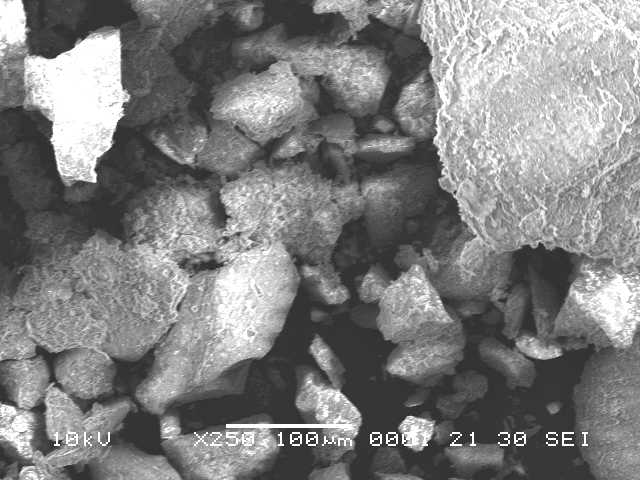
\includegraphics[width=\linewidth]{HKI_natural_azurite_x250_3_040521}
\end{minipage}
\begin{minipage}{.45\textwidth}
  \centering
  \includegraphics[width=\linewidth]{HKI_natural_azurite_x250_5_040521}
\end{minipage}
\caption[SEM images: Sample HKI, natural azurite]{SEM images: Sample HKI, natural azurite. Magnification: 250x.}
\label{fig:hki_nat_az_sem_1}
\end{figure}

It is possible to see the surface texture of larger particles more clearly at 750x magnification in \textit{Figure \ref{fig:hki_nat_az_sem_2}}. It appears that there are smaller particles embedded in or settled on the surface of larger particles, making a rough surface. Particles have clearly sharp angular edges and are not rounded. At this magnification the large variation in particle size is apparent, and the asymmetry of the material is noted.

\begin{figure}[H]
\centering
\begin{minipage}{.45\textwidth}
  \centering
  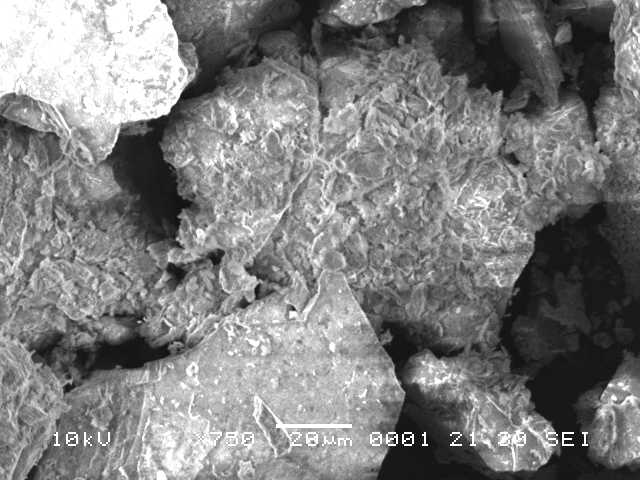
\includegraphics[width=\linewidth]{HKI_natural_azurite_x750_1_040521}
\end{minipage}
\begin{minipage}{.45\textwidth}
  \centering
  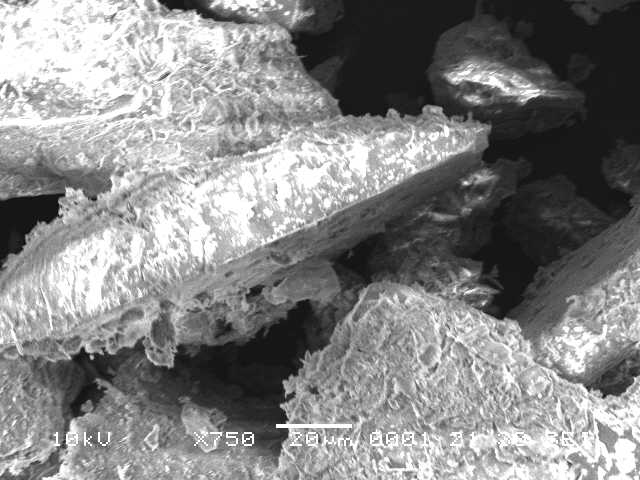
\includegraphics[width=\linewidth]{HKI_natural_azurite_x750_3_040521}
\end{minipage}
\caption[SEM images: Sample HKI, natural azurite]{SEM images: Sample HKI, natural azurite. Magnification: 750x.}
\label{fig:hki_nat_az_sem_2}
\end{figure}

The fine surface detail on the flat sides of larger particles can be observed at 1500x magnification in \textit{Figure \ref{fig:hki_nat_az_sem_3}}. The image on the right shows several more spherical looking particles, though many more appear asymmetrical with uneven sharp edges. The size of the texture on the surface is consistent in size in contrast to the macro size heterogeneity.

\begin{figure}[H]
\centering
\begin{minipage}{.45\textwidth}
  \centering
  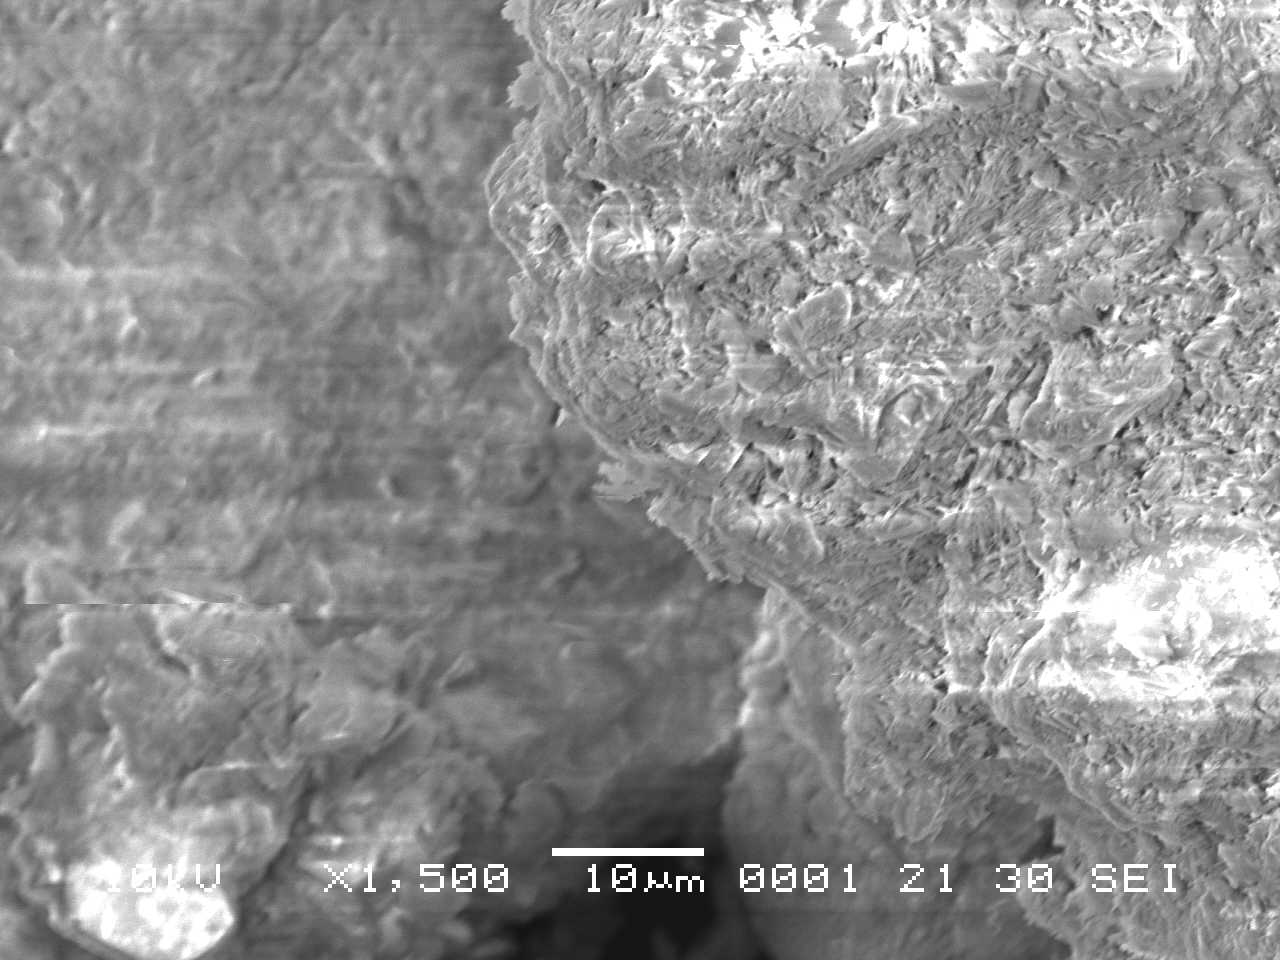
\includegraphics[width=\linewidth]{HKI_natural_azurite_x1500_2_040521}
\end{minipage}
\begin{minipage}{.45\textwidth}
  \centering
  \includegraphics[width=\linewidth]{HKI_natural_azurite_x1500_4_040521}
\end{minipage}
\caption[SEM images: Sample HKI, natural azurite]{SEM images: Sample HKI, natural azurite. Magnification: 1500x.}
\label{fig:hki_nat_az_sem_3}
\end{figure}

\textit{Figure \ref{fig:hki_nat_az_sem_4}} shows two images at 2000x magnification. The image on the right shows clear sharp-sided particles. These are extremely uneven. The left image, on the other hand, shows flat irregular small particles layered over one another like flakes.

\begin{figure}[H]
\centering
\begin{minipage}{.45\textwidth}
  \centering
  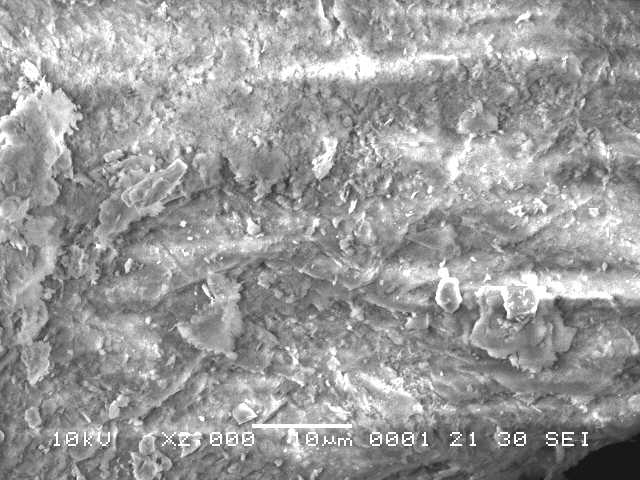
\includegraphics[width=\linewidth]{HKI_natural_azurite_x2000_1_040521}
\end{minipage}
\begin{minipage}{.45\textwidth}
  \centering
  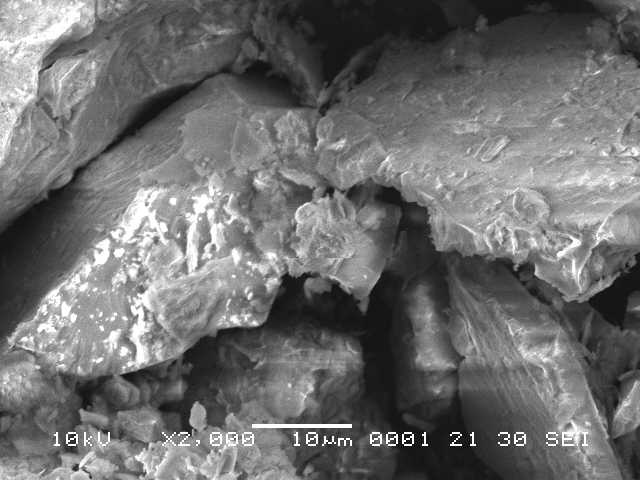
\includegraphics[width=\linewidth]{HKI_natural_azurite_x2000_3_040521}
\end{minipage}
\caption[SEM images: Sample HKI, natural azurite]{SEM images: Sample HKI, natural azurite. Magnification: 2000x.}
\label{fig:hki_nat_az_sem_4}
\end{figure}

At very high magnification (4000x), \textit{Figure \ref{fig:hki_nat_az_sem_5}} shows the fine structure of the sample very clearly. There is still significant size variation at this magnification, and interesting needle like crystal formations are observed. These do appear to be orientated in some places, possibly showing the areas of crystal nucleation and growth. Other needle like crystals appear randomly orientated. Notably, this ordering is not readily observed in other samples, though needle like crystals are.

\begin{figure}[H]
\centering
\begin{minipage}{.45\textwidth}
  \centering
  \includegraphics[width=\linewidth]{HKI_natural_azurite_x4000_2_040521}
\end{minipage}
\begin{minipage}{.45\textwidth}
  \centering
  \includegraphics[width=\linewidth]{HKI_natural_azurite_x4000_5_040521}
\end{minipage}
\caption[SEM images: Sample HKI, natural azurite]{SEM images: Sample HKI, natural azurite. Magnification: 4000x.}
\label{fig:hki_nat_az_sem_5}
\end{figure}

% ************************************************     Az1     *******************************************************************

Sample Az1, likely from a natural source, is shown in \textit{Figures \ref{fig:az1_sem_1}} and \textit{\ref{fig:az1_sem_2}}. 

\textit{Figure \ref{fig:az1_sem_1}}, at 750x magnification, shows significant size variation in the sample. There are many flat, sharp particles as well as many smaller particles. It is difficult to determine whether the larger pieces of sample are aggregates of smaller particles or larger intact pieces; the surfaces of these appear almost pocked, especially in the left image.

\begin{figure}[H]
\centering
\begin{minipage}{.45\textwidth}
  \centering
  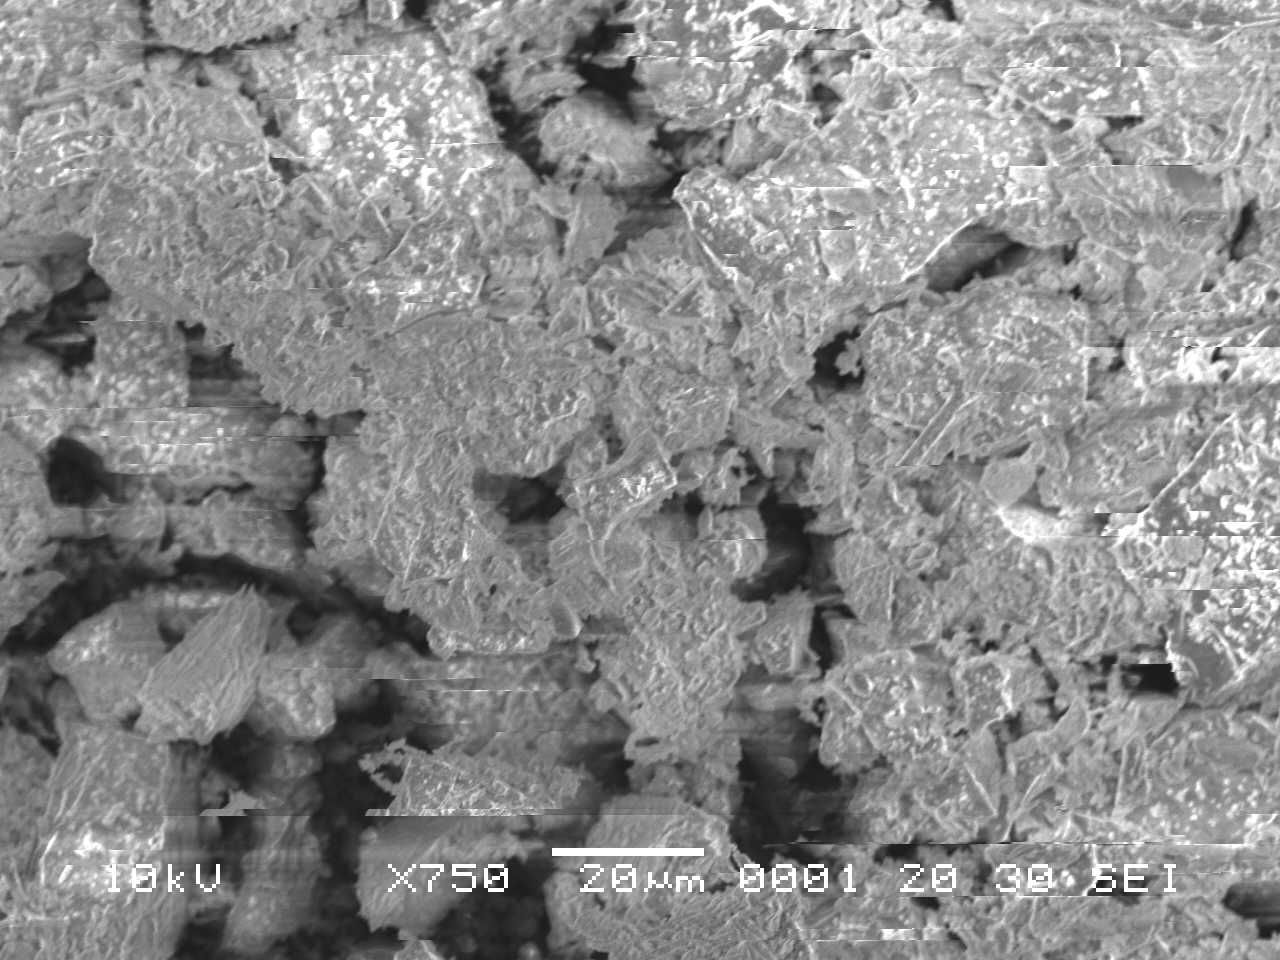
\includegraphics[width=\linewidth]{Az1_x750_3_220221}
\end{minipage}
\begin{minipage}{.45\textwidth}
  \centering
  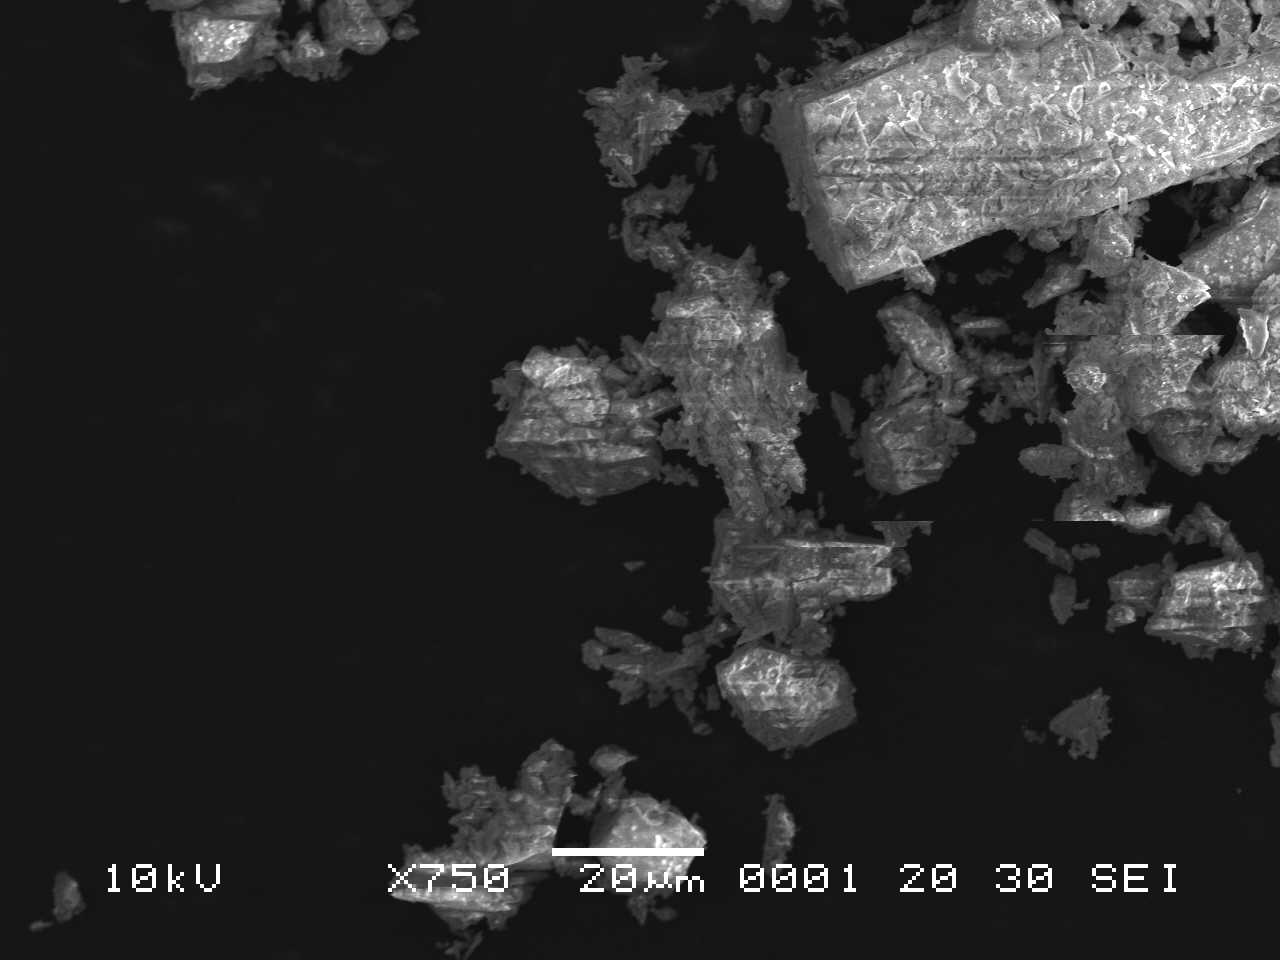
\includegraphics[width=\linewidth]{Az1_x750_6_220221}
\end{minipage}
\caption[SEM images: Sample Az1, azurite]{SEM images: Sample Az1, azurite. Magnification: 750x.}
\label{fig:az1_sem_1}
\end{figure}

\textit{Figure \ref{fig:az1_sem_2}} shows Az1 at 1500x (left) and 2000x (right). At 1500x, it is possible to observe smaller voluminous (not flat) particles on the surface of larger particles. The vast majority of pieces are irregularly shaped with choppy borders, though a few circular particles are also present. At 2000x, the image shows the flat edge of a larger particle. There is a great deal of surface texture, as well as some intriguing grid formations that do not appear to be artifacts of the SEM. These may be due to grinding and polishing of the pigment, but also may suggest some crytal ordering. Uniformity of shape and size is low at all magnifications and all over the sample.

\begin{figure}[H]
\centering
\begin{minipage}{.45\textwidth}
  \centering
  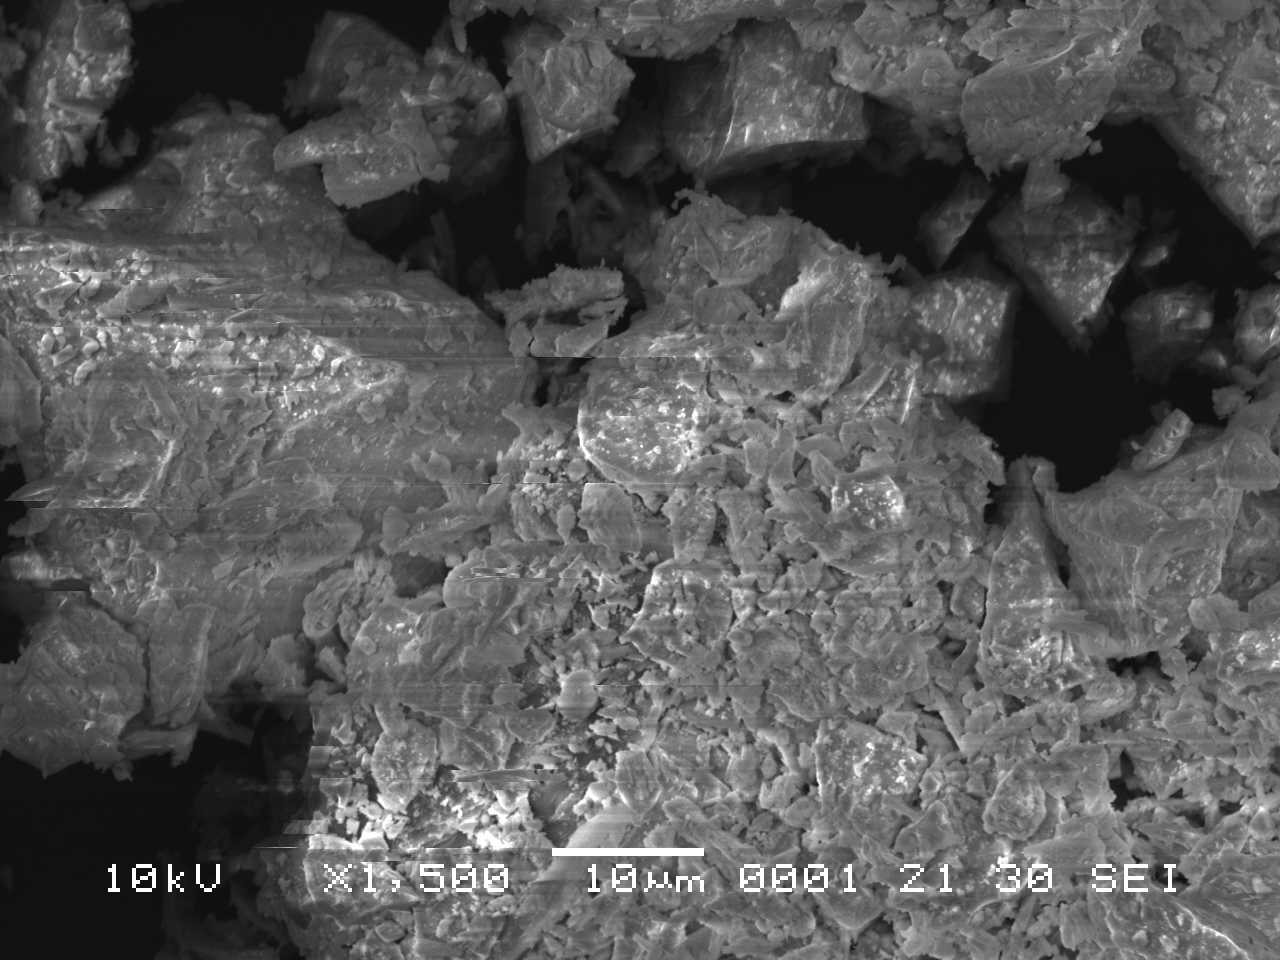
\includegraphics[width=\linewidth]{Az1_x1500_2_220221}
\end{minipage}
\begin{minipage}{.45\textwidth}
  \centering
  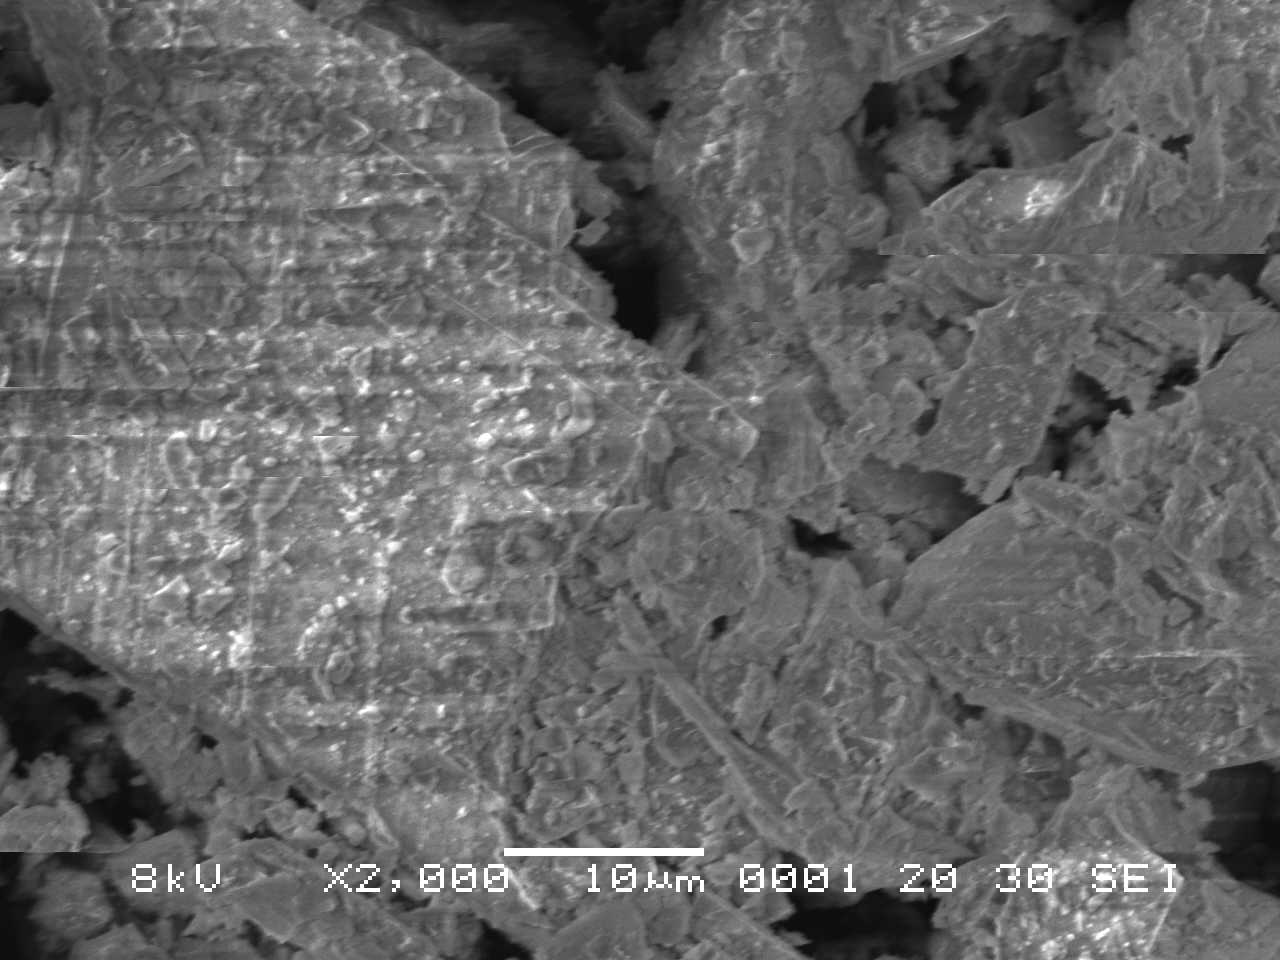
\includegraphics[width=\linewidth]{Az1_x2000_4_220221}
\end{minipage}
\caption[SEM images: Sample Az1, azurite]{SEM images: Sample Az1, azurite. Magnification: \textbf{left)} 1500x, \textbf{right)} 2000x}
\label{fig:az1_sem_2}
\end{figure}

% ************************************************     Az2     *******************************************************************

\textit{Figures \ref{fig:az2_sem_1}} and \textit{\ref{fig:az2_sem_2}} show sample Az2, which is morphologically significantly different from all other observed samples and lacks the features that appear to correlate with either natural or artificial pigment sources. Surface charging made it difficult to image this sample, and this issue was also not observed with most other samples.

In \textit{Figure \ref{fig:az2_sem_1}}, two images of the sample at 200x magnification are shown. It is interesting that although the shape of each sample is quite asymmetric and angular, the size and irregular shape is quite consistent between particules. At this magnification, the surface of the particles appears flat and smooth. It is also significant that these particles are much larger than the average particle size observed in other samples, which may suggest industrial pigment grinding. Otherwise, this consistency could also reflect a synthetic origin, with controlled conditions of crystal growth.

\begin{figure}[H]
\centering
\begin{minipage}{.45\textwidth}
  \centering
  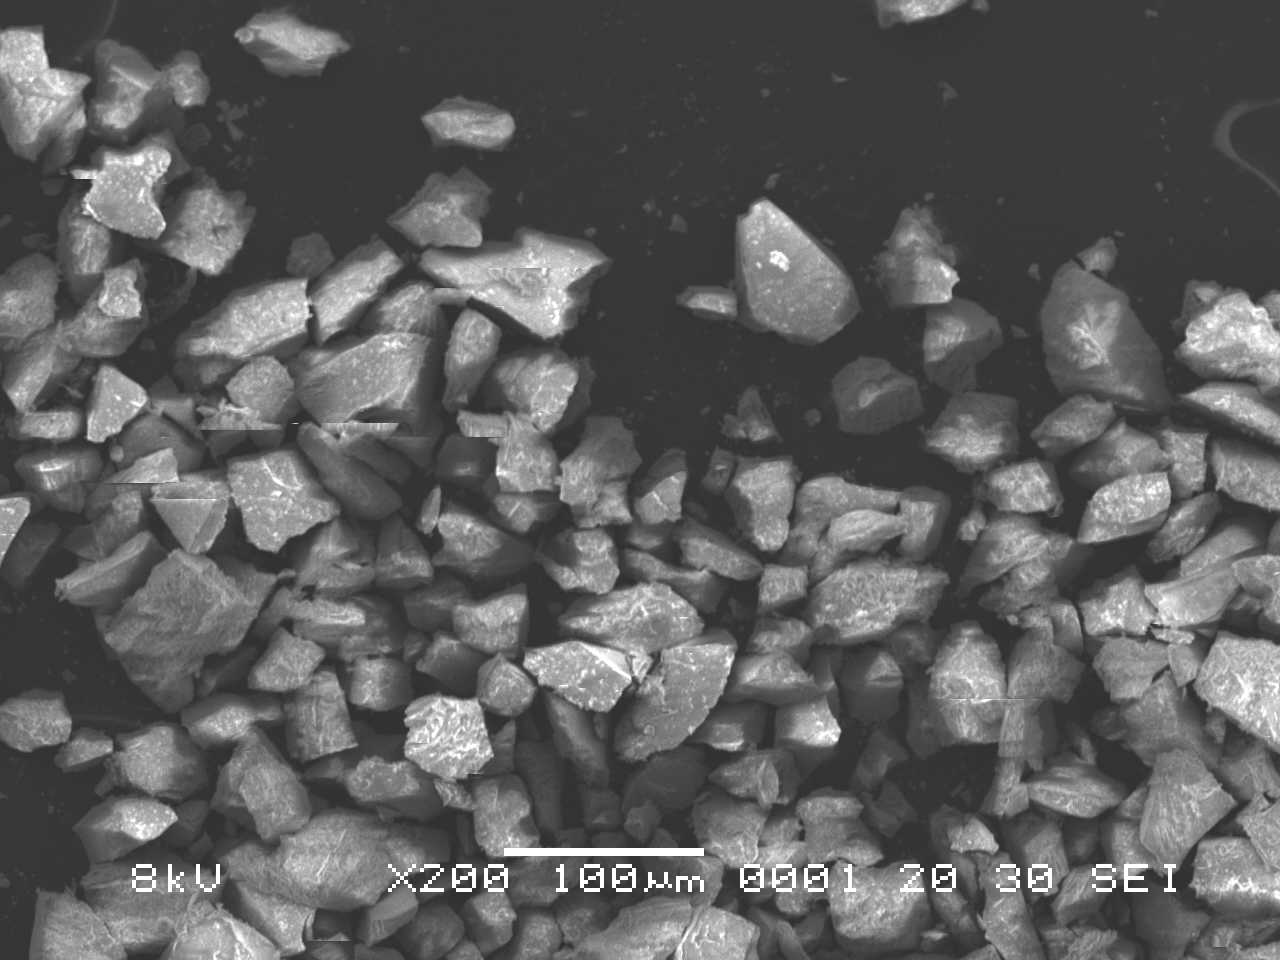
\includegraphics[width=\linewidth]{Az2_x200_1_240221}
\end{minipage}
\begin{minipage}{.45\textwidth}
  \centering
  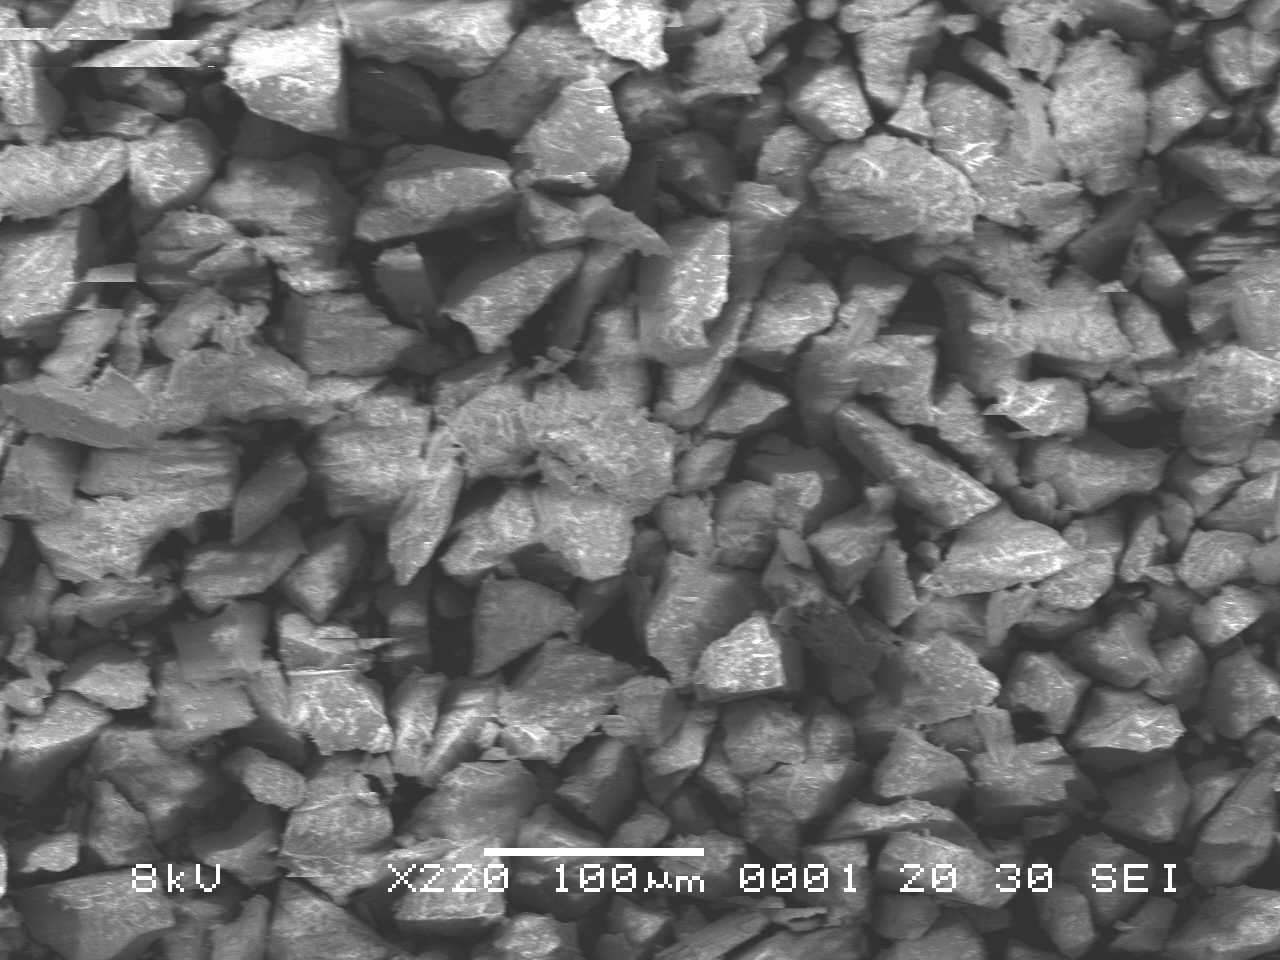
\includegraphics[width=\linewidth]{Az2_x200_2_240221}
\end{minipage}
\caption[SEM images: Sample Az2, azurite]{SEM images: Sample Az2, azurite. Magnification: 200x.}
\label{fig:az2_sem_1}
\end{figure}

In \textit{Figure \ref{fig:az2_sem_2}}, Az2 is shown at 750x (left) and 1500x (right). Imaging at higher magnifications was not possible due to charging. At 750x magnification, relatively flat sides of particles are observed. There is slightly more size variation than initially seen, though this is difficult to assess due to jumping of particles during charging. At 1500x magnification, there is very little surface texture observed. Sample Az2 is obviously unlike the sample HKI natural azurite. However, it also does not resemble known synthetic samples either. 

\begin{figure}[H]
\centering
\begin{minipage}{.45\textwidth}
  \centering
  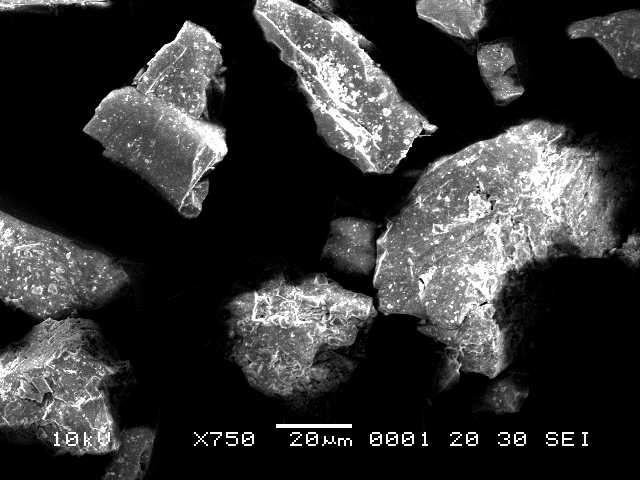
\includegraphics[width=\linewidth]{Az2_x750_1_150321}
\end{minipage}
\begin{minipage}{.45\textwidth}
  \centering
  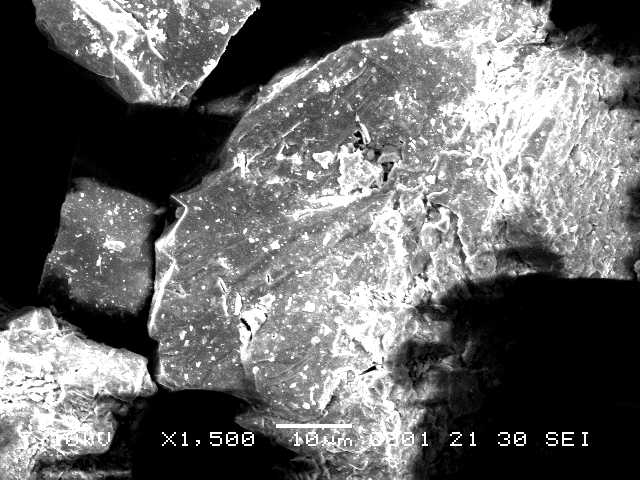
\includegraphics[width=\linewidth]{Az2_x1500_1_150321}
\end{minipage}
\caption[SEM images: Sample Az2, azurite]{SEM images: Sample Az2, azurite. Magnification: \textbf{left)} 750x, \textbf{right)} 1500x}
\label{fig:az2_sem_2}
\end{figure}

% ************************************************     AzMag     *******************************************************************

\textit{Figures \ref{fig:azmag_sem_1}-\ref{fig:azmag_sem_5}} show sample AzMag at magnifications from 200x to 4000x. 

At 200-250x magnification (\textit{Figure \ref{fig:azmag_sem_1}}), extremely small particles are shown. The particle size is fairly homogeneous, though there is a great deal of variation in particle shape as well as a lot of texture observed.

\begin{figure}[H]
\centering
\begin{minipage}{.45\textwidth}
  \centering
  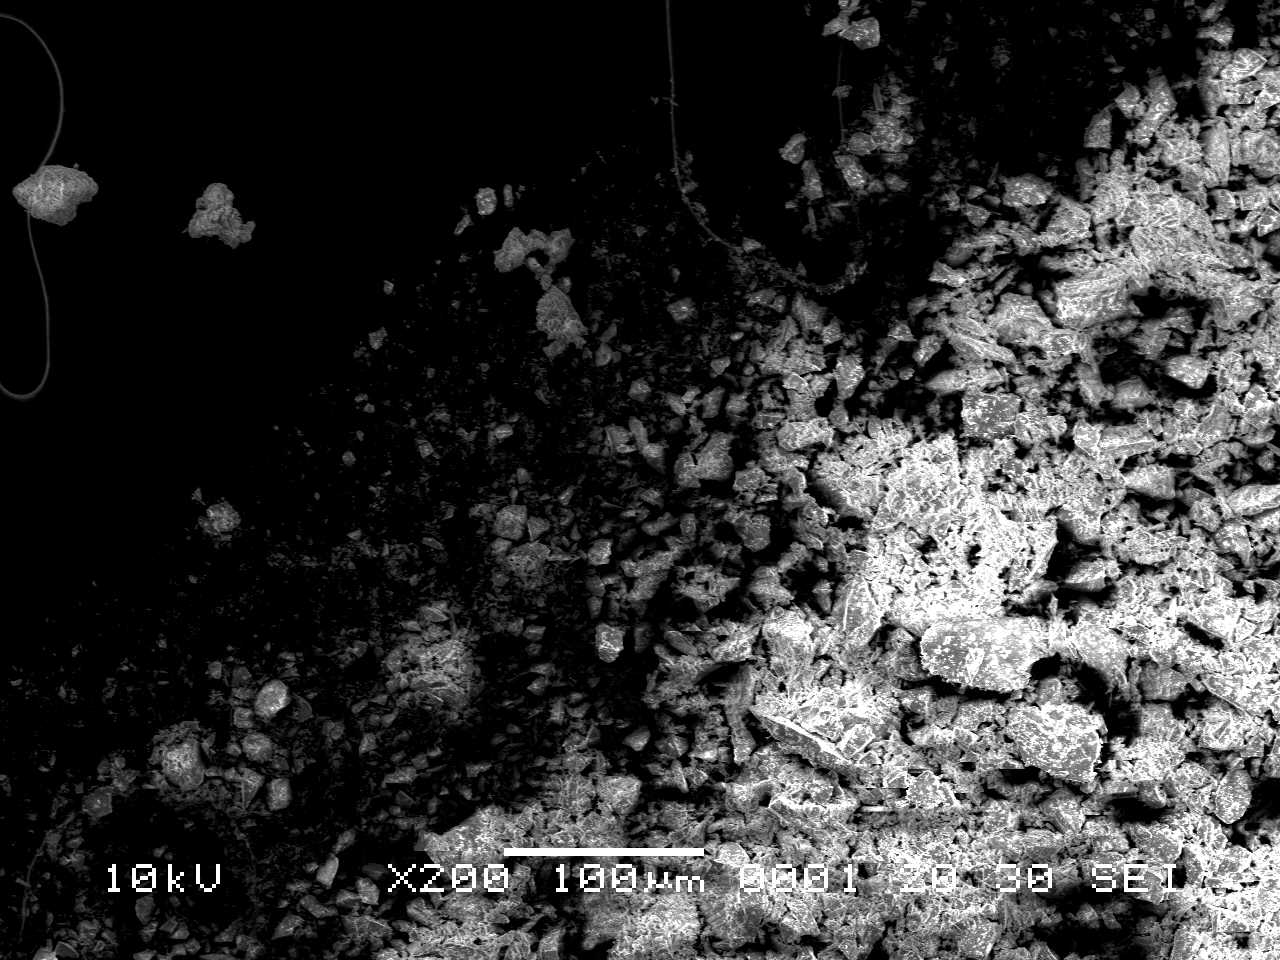
\includegraphics[width=\linewidth]{AzMag_x200_1_260221}
\end{minipage}
\begin{minipage}{.45\textwidth}
  \centering
  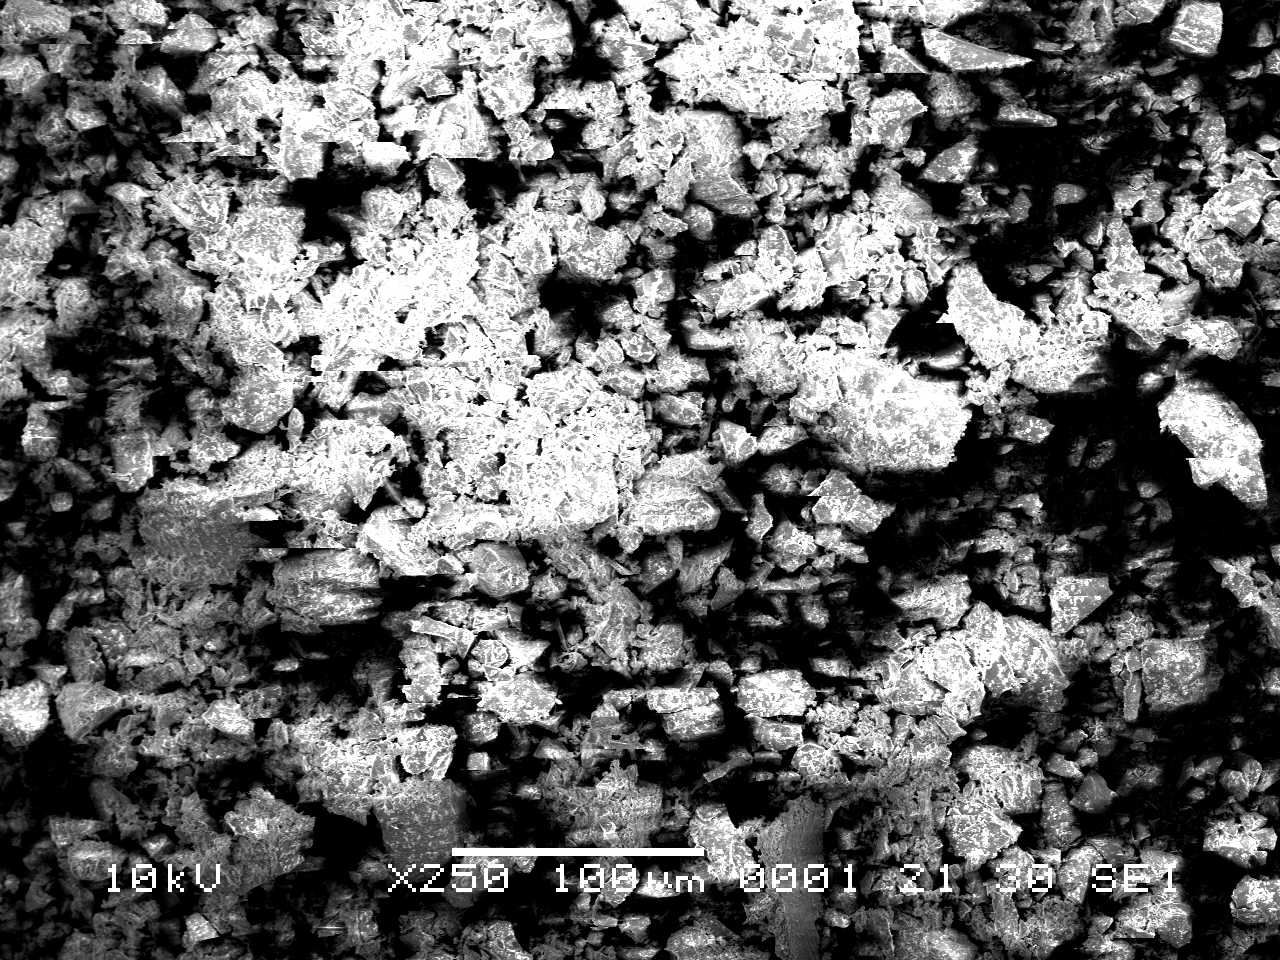
\includegraphics[width=\linewidth]{AzMag_x250_2_160321}
\end{minipage}
\caption[SEM images: Sample AzMag, azurite]{SEM images: Sample AzMag, azurite. Magnification: \textbf{left)} 200x, \textbf{right)} 250x}
\label{fig:azmag_sem_1}
\end{figure}

\textit{Figure \ref{fig:azmag_sem_2}} shows the sample at 750x magnification. The surfaces are choppy, rough, and highly textured. Most particles are approximately square or triangular, with a few small spheres on the surface. Elongated and large particles are not observed.

\begin{figure}[H]
\centering
\begin{minipage}{.45\textwidth}
  \centering
  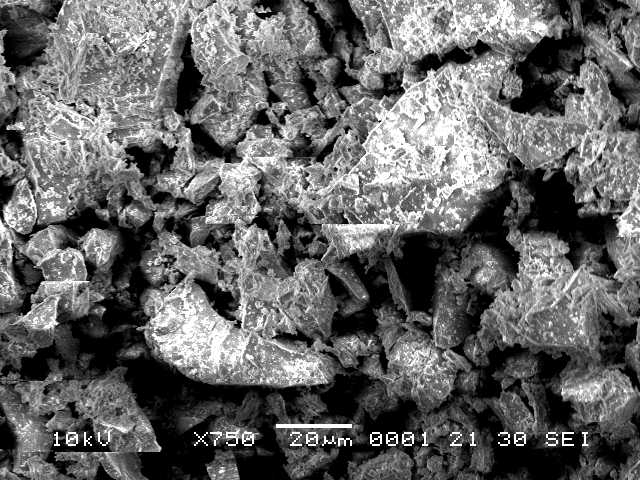
\includegraphics[width=\linewidth]{AzMag_x750_1_160321}
\end{minipage}
\begin{minipage}{.45\textwidth}
  \centering
  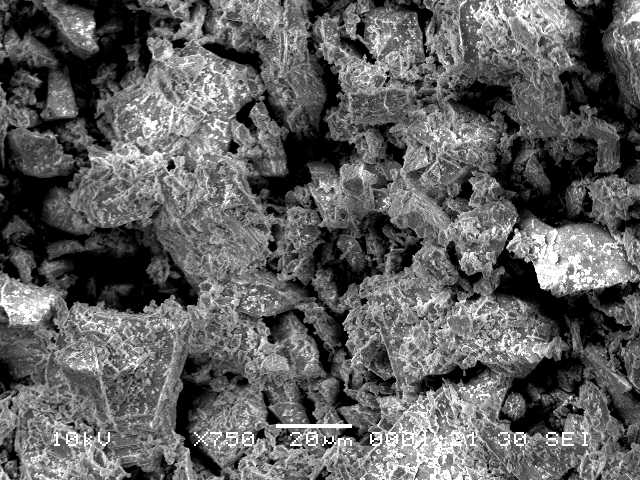
\includegraphics[width=\linewidth]{AzMag_x750_3_160321}
\end{minipage}
\caption[SEM images: Sample AzMag, azurite]{SEM images: Sample AzMag, azurite. Magnification: 750x}
\label{fig:azmag_sem_2}
\end{figure}

\textit{Figure \ref{fig:azmag_sem_3}} and the left image in \textit{Figure \ref{fig:azmag_sem_4}} show the sample at 1500x magnification. Here, sample AzMag is qualitatively similar to HKI natural azurite. There are thinnner forms, though they are not quite as delicate as the needle like formations discussed previously. 

\begin{figure}[H]
\centering
\begin{minipage}{.45\textwidth}
  \centering
  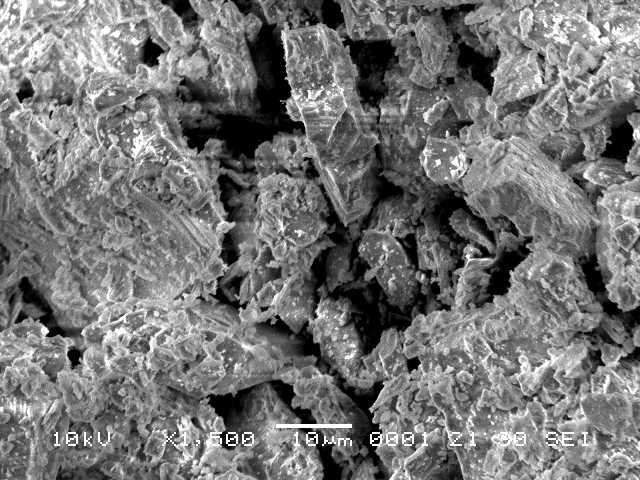
\includegraphics[width=\linewidth]{AzMag_x1500_1_160321}
\end{minipage}
\begin{minipage}{.45\textwidth}
  \centering
  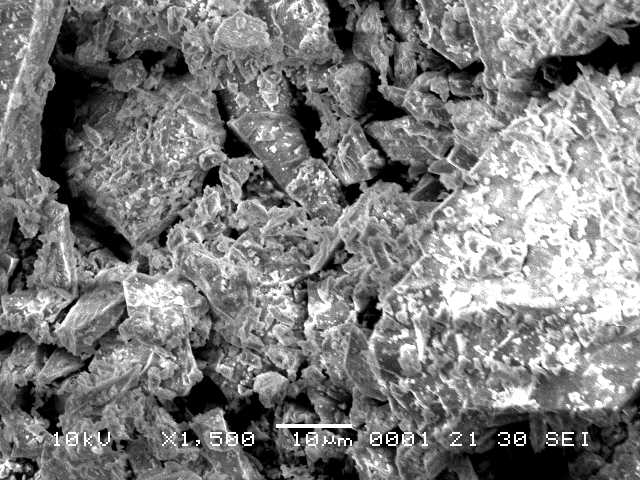
\includegraphics[width=\linewidth]{AzMag_x1500_3_160321}
\end{minipage}
\caption[SEM images: Sample AzMag, azurite]{SEM images: Sample AzMag, azurite. Magnification: 1500x}
\label{fig:azmag_sem_3}
\end{figure}

\begin{figure}[H]
\centering
\begin{minipage}{.45\textwidth}
  \centering
  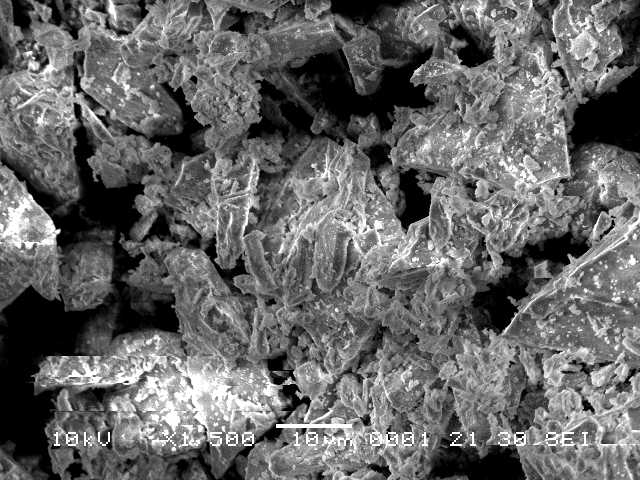
\includegraphics[width=\linewidth]{AzMag_x1500_5_160321}
\end{minipage}
\begin{minipage}{.45\textwidth}
  \centering
  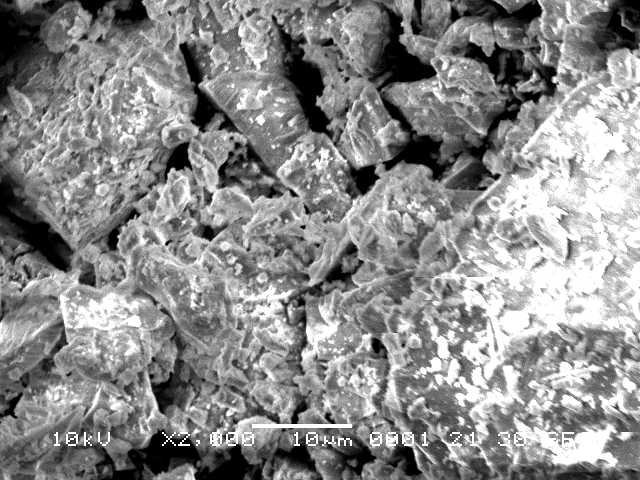
\includegraphics[width=\linewidth]{AzMag_x2000_1_160321}
\end{minipage}
\caption[SEM images: Sample AzMag, azurite]{SEM images: Sample AzMag, azurite. Magnification: \textbf{left)} 1500x, \textbf{right)} 2000x}
\label{fig:azmag_sem_4}
\end{figure}

At high magnification, the surface texture of the sample is clearly visualized. \textit{Figure \ref{fig:azmag_sem_5}} shows elongated, narrow crystals at 3000x (left) and 4000x (right). The directionality observed in HKI natural azurite at high magnifications is not observed here. However, the degree of roughness and character of the surfaces is very similar, implying that this sample is naturally produced.

\begin{figure}[H]
\centering
\begin{minipage}{.45\textwidth}
  \centering
  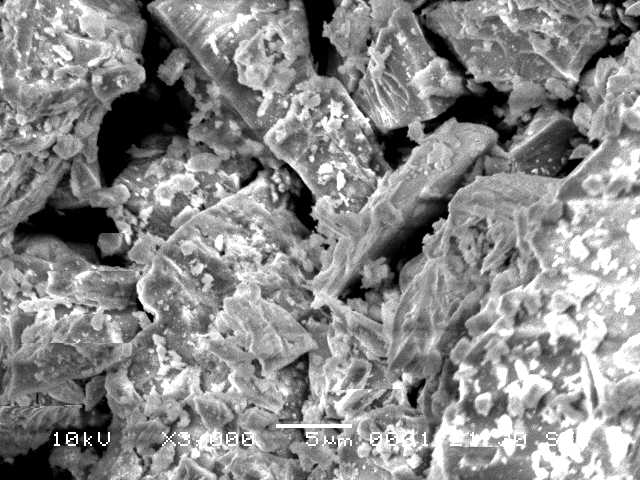
\includegraphics[width=\linewidth]{AzMag_x3000_1_160321}
\end{minipage}
\begin{minipage}{.45\textwidth}
  \centering
  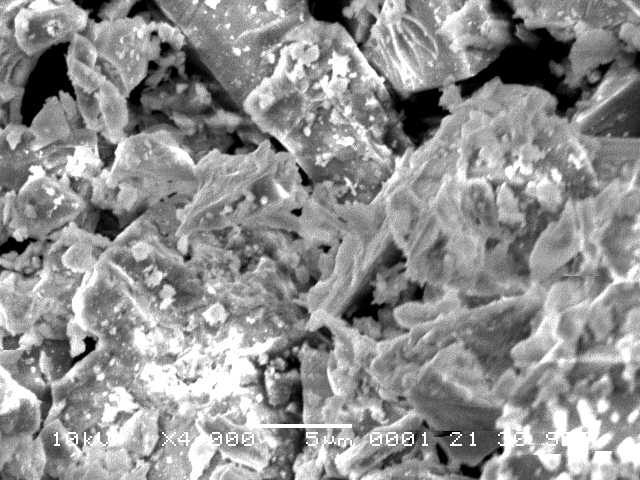
\includegraphics[width=\linewidth]{AzMag_x4000_1_160321}
\end{minipage}
\caption[SEM images: Sample AzMag, azurite]{SEM images: Sample AzMag, azurite. Magnification: \textbf{left)} 3000x, \textbf{right)} 4000x}
\label{fig:azmag_sem_5}
\end{figure}

% ************************************************     AzOp     *******************************************************************

\textit{Figures \ref{fig:azop_sem_1}-\ref{fig:azop_sem_3}} show sample AzOp at magnifications from 250x to 2000x. 

At 250x magnification (\textit{Figure \ref{fig:azop_sem_1}}, left), small and very textured particles are observed. The size of these particles is fairly homogenous. At 750x magnification (\textit{Figure \ref{fig:azop_sem_1}}, right), it is clear that there are larger particles/aggregations. It is difficult to tell whether these are in fact single pieces or clumps of smaller particles. The shape of all particles is extremely asymmetrical and varied, except in one specific case; at the bottom of the image there is a cluster of fairly uniformly spherical particles. 

\begin{figure}[H]
\centering
\begin{minipage}{.45\textwidth}
  \centering
  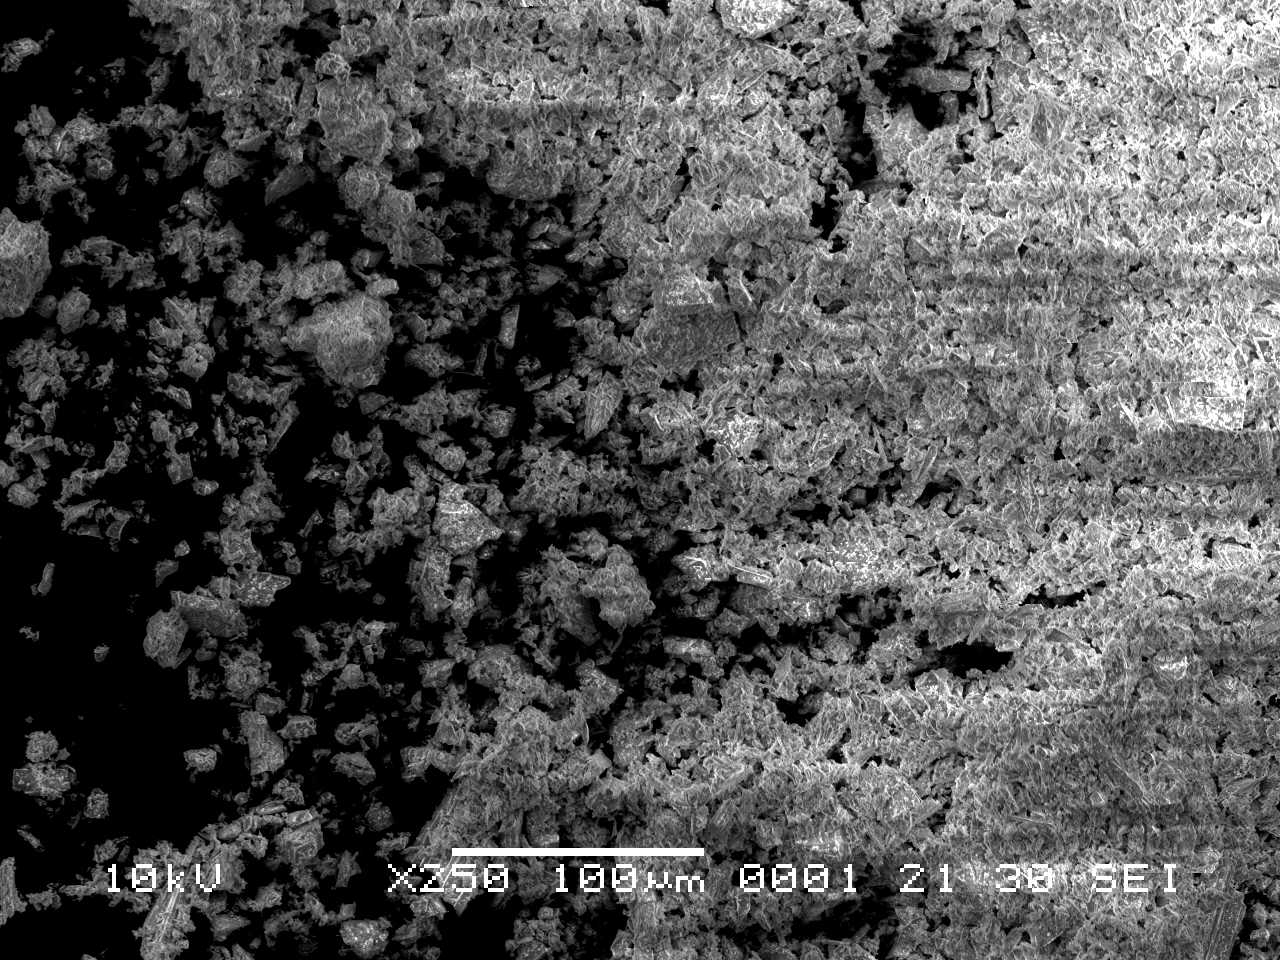
\includegraphics[width=\linewidth]{AzOp_x250_1_150321}
\end{minipage}
\begin{minipage}{.45\textwidth}
  \centering
  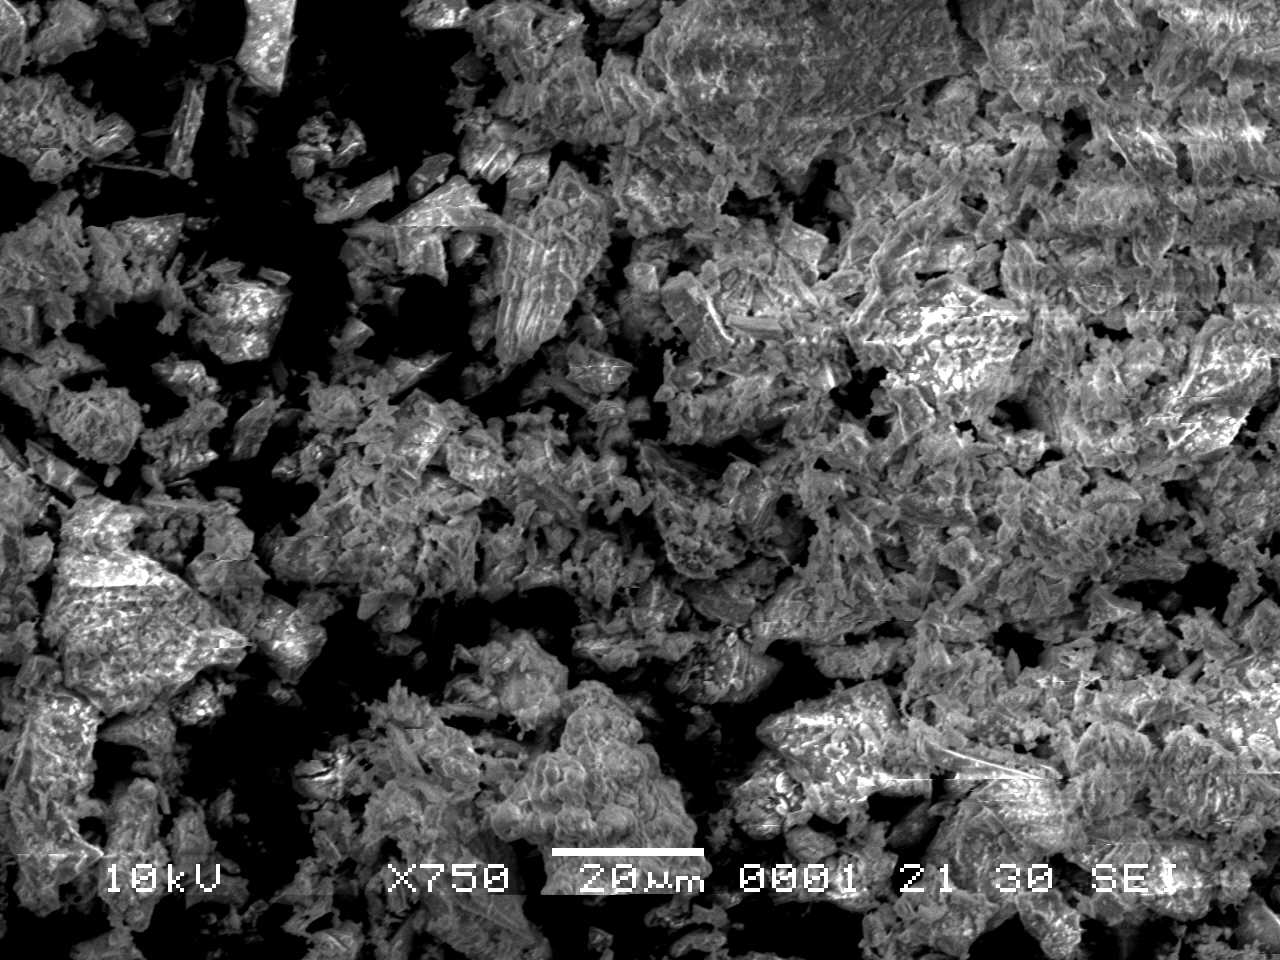
\includegraphics[width=\linewidth]{AzOp_x750_2_150321}
\end{minipage}
\caption[SEM images: Sample AzOp, azurite]{SEM images: Sample AzOp, azurite. Magnification: \textbf{left)} 250x, \textbf{right)} 750x}
\label{fig:azop_sem_1}
\end{figure}

The spherical particles are clearly observed in \textit{Figure \ref{fig:azop_sem_2}}, left, and \textit{Figure \ref{fig:azop_sem_3}}, right. They appear bubbly, as if many partial spheres have formed one on top of the other. This texture is not observed extensively in this sample, nor in other samples such as AzMag and HKI natural azurite that are otherwise similar to the rest of sample AzOp. This could be the result of sample contamination, as several samples were analyzed at the same time, or this could be evidence of multiple conditions under which crystals formed before being mixed to make this pigment. Regardless, this type of morphology is quite uniform and does not look like the result of random crushing and grinding. This certainly must be investigated further by imaging over a larger area of this sample as well as by preparing additional fresh samples.

In contrast, the rougher and more heterogenous texture of the majority of the sample is shown at 2000x magnification in \textit{Figure \ref{fig:azop_sem_3}}, left, and at 4000x magnification in \textit{Figure \ref{fig:azop_sem_2}}, right. Very few remotely circular particles are seen, and there is a great deal of heterogeneity in size and shape. This is very similar to natural samples discussed above.

\begin{figure}[H]
\centering
\begin{minipage}{.45\textwidth}
  \centering
  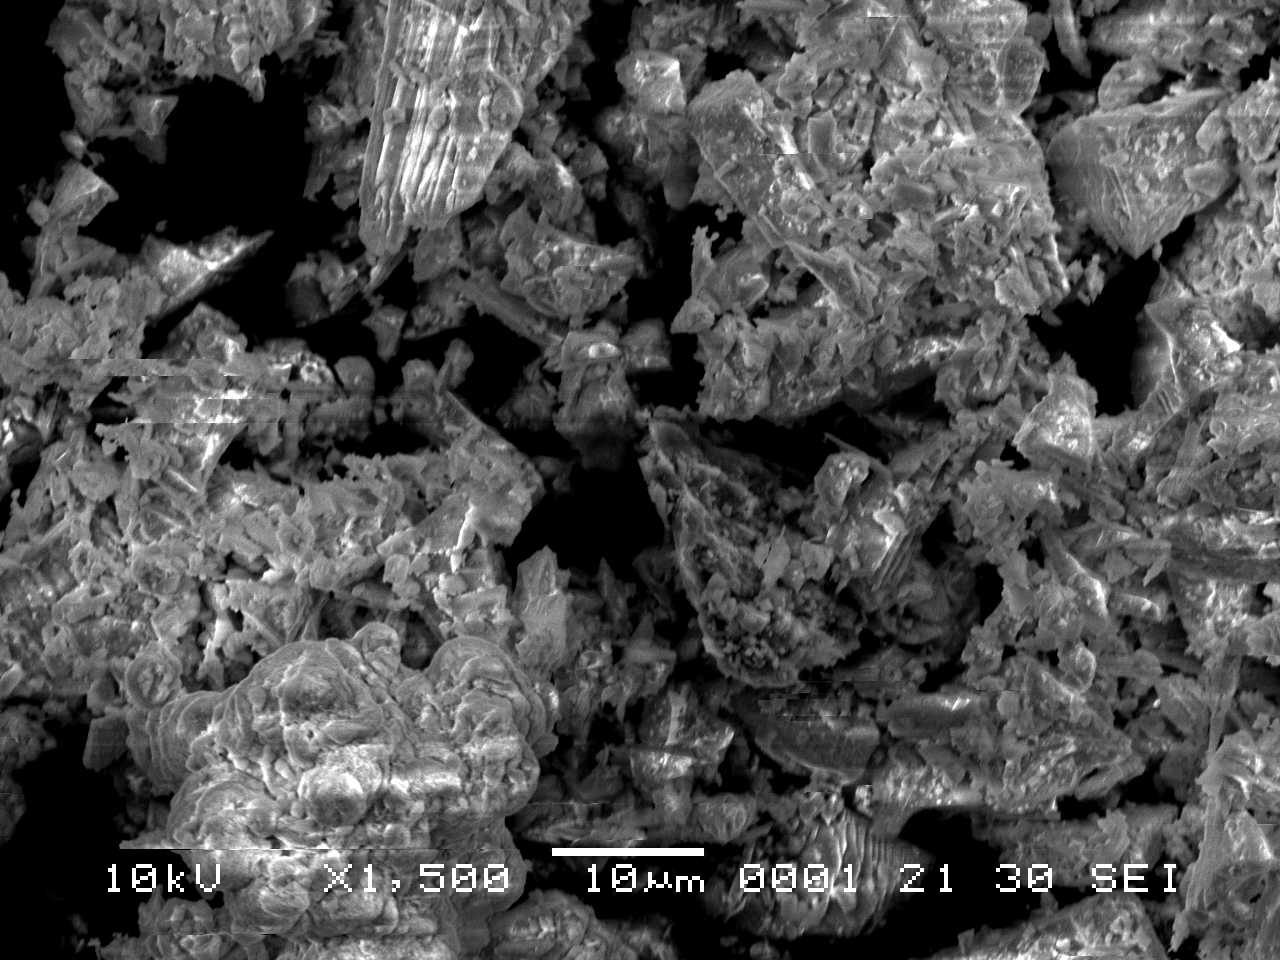
\includegraphics[width=\linewidth]{AzOp_x1500_2_150321}
\end{minipage}
\begin{minipage}{.45\textwidth}
  \centering
  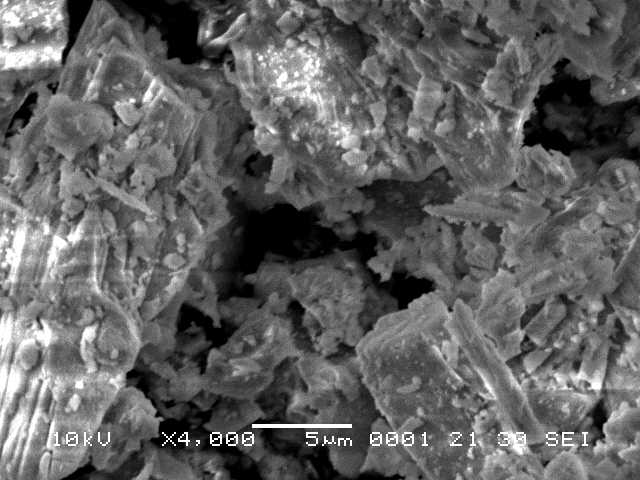
\includegraphics[width=\linewidth]{AzOp_x4000_1_150321}
\end{minipage}
\caption[SEM images: Sample AzOp, azurite]{SEM images: Sample AzOp, azurite. Magnification: \textbf{left)} 1500x, \textbf{right)} 4000x}
\label{fig:azop_sem_2}
\end{figure}

\begin{figure}[H]
\centering
\begin{minipage}{.45\textwidth}
  \centering
  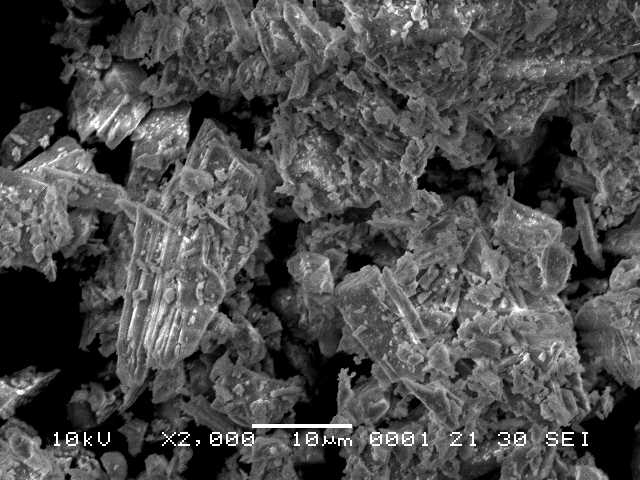
\includegraphics[width=\linewidth]{AzOp_x2000_1_150321}
\end{minipage}
\begin{minipage}{.45\textwidth}
  \centering
  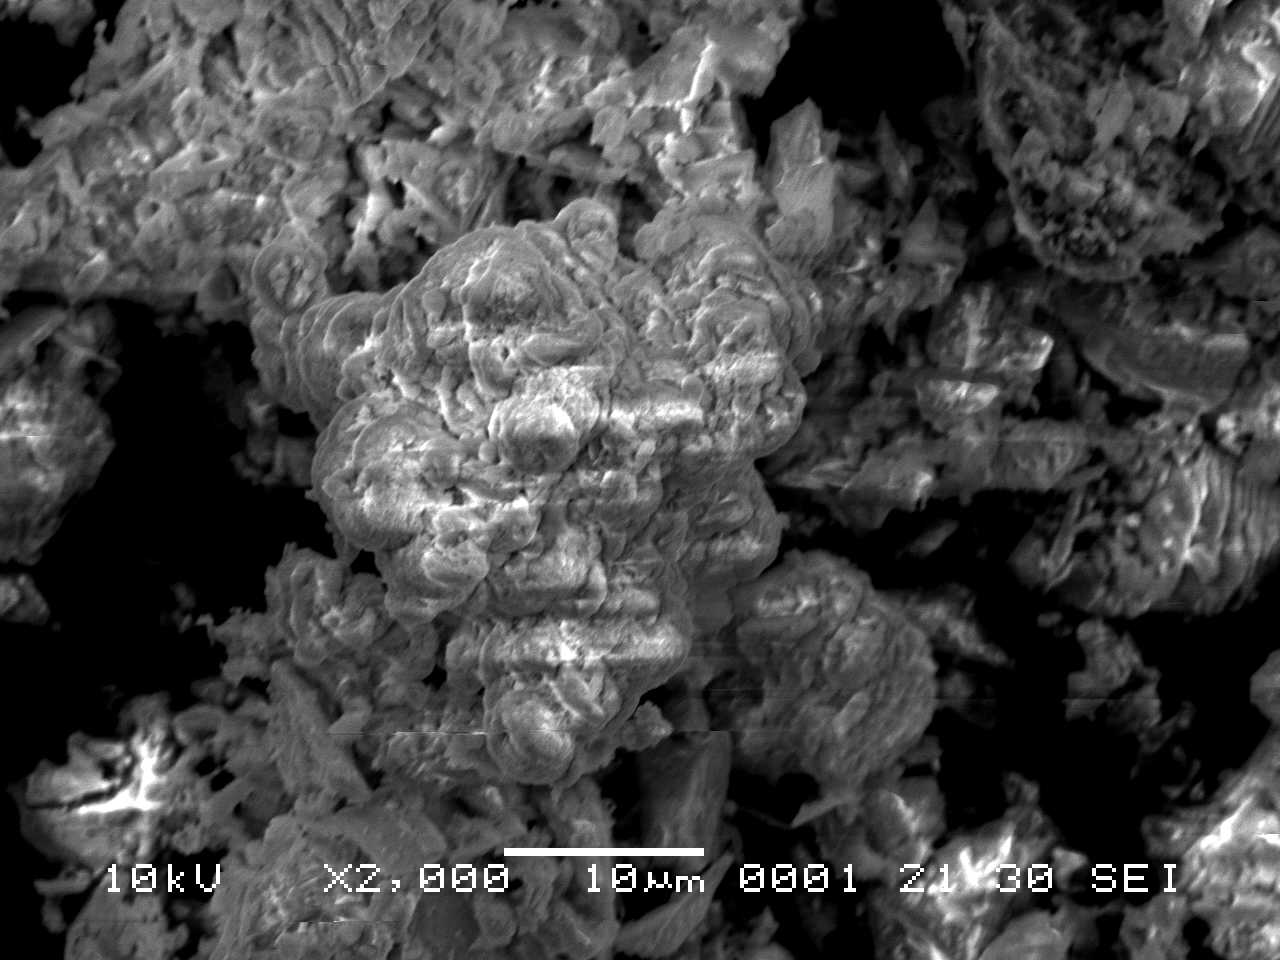
\includegraphics[width=\linewidth]{AzOp_x2000_4_150321}
\end{minipage}
\caption[SEM images: Sample AzOp, azurite]{SEM images: Sample AzOp, azurite. Magnification: 2000x}
\label{fig:azop_sem_3}
\end{figure}

% ************************************************     Fitz1     *******************************************************************
\todo{can you use NLP or ML to do this kind of pattern recognization?? this could be good to look into further.}

\textit{Figures \ref{fig:Fitz1_sem_1}} and \textit{Figure \ref{fig:Fitz1_sem_2}} show sample Fitz1 at magnifications from 250x to 2500x. This sample is described as blue verditer, and a commercial product number is provided allowing confirmation that this is a synthetic product.

At 250x magnification (\textit{Figure \ref{fig:Fitz1_sem_1}}, left), small uniform particles are seen. These appear generally circular and far more consistent in size and shape than the samples discussed thus far. At 750x magnification (\textit{Figure \ref{fig:Fitz1_sem_1}}, right), it is possible to qualitatively assess the diameter of particles as consistently < 5 $\mu$m. Particles resemble the spherical cluster observed in the sample AzOp. There is regularity of both size and shape, but it is difficult to determine whether the particles are flat discs or stacked semicircles occupying more volume.

\begin{figure}[H]
\centering
\begin{minipage}{.45\textwidth}
  \centering
  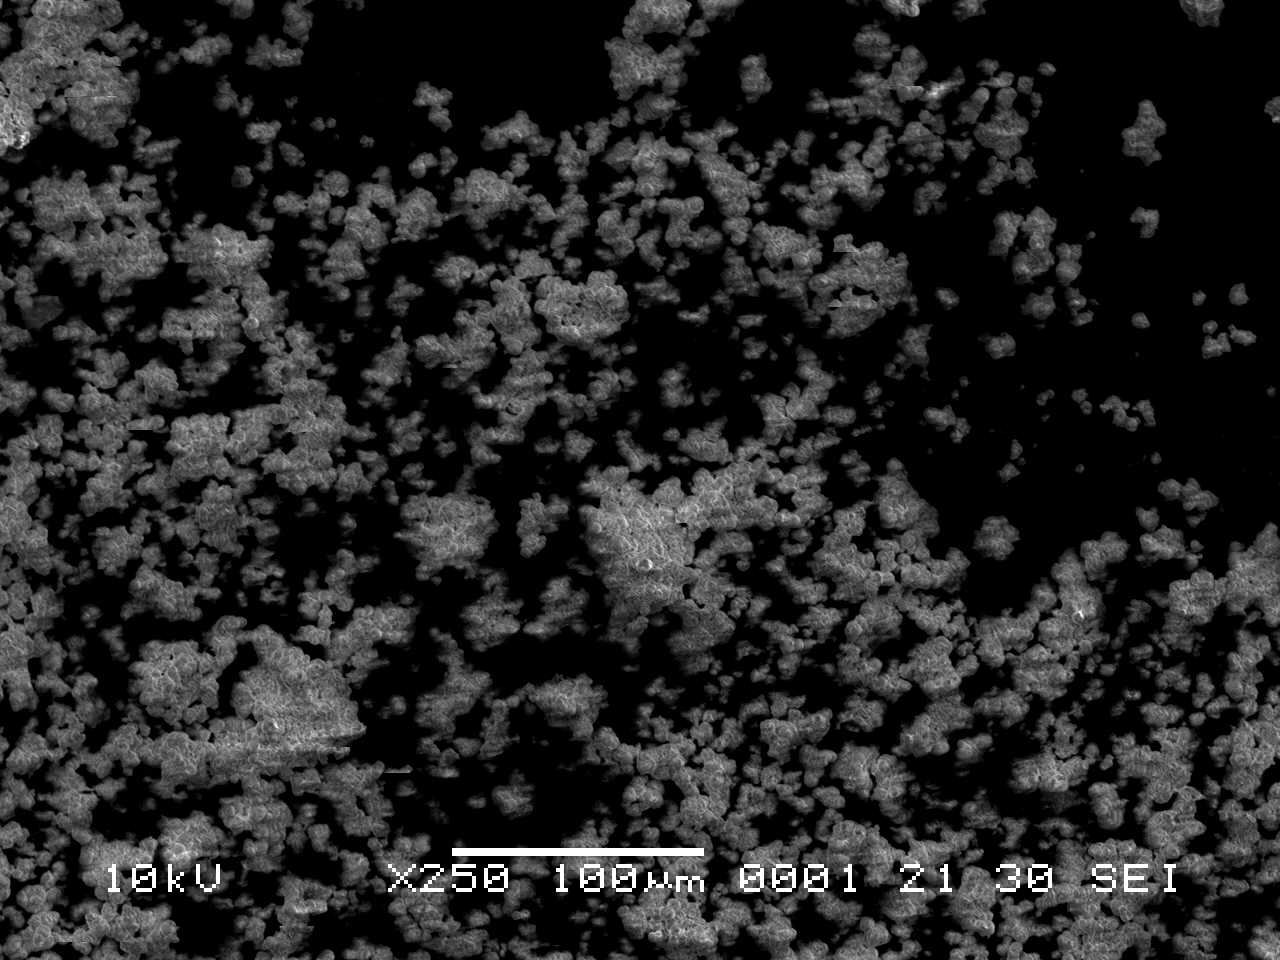
\includegraphics[width=\linewidth]{Fitz1_x250_1_030321}
\end{minipage}
\begin{minipage}{.45\textwidth}
  \centering
  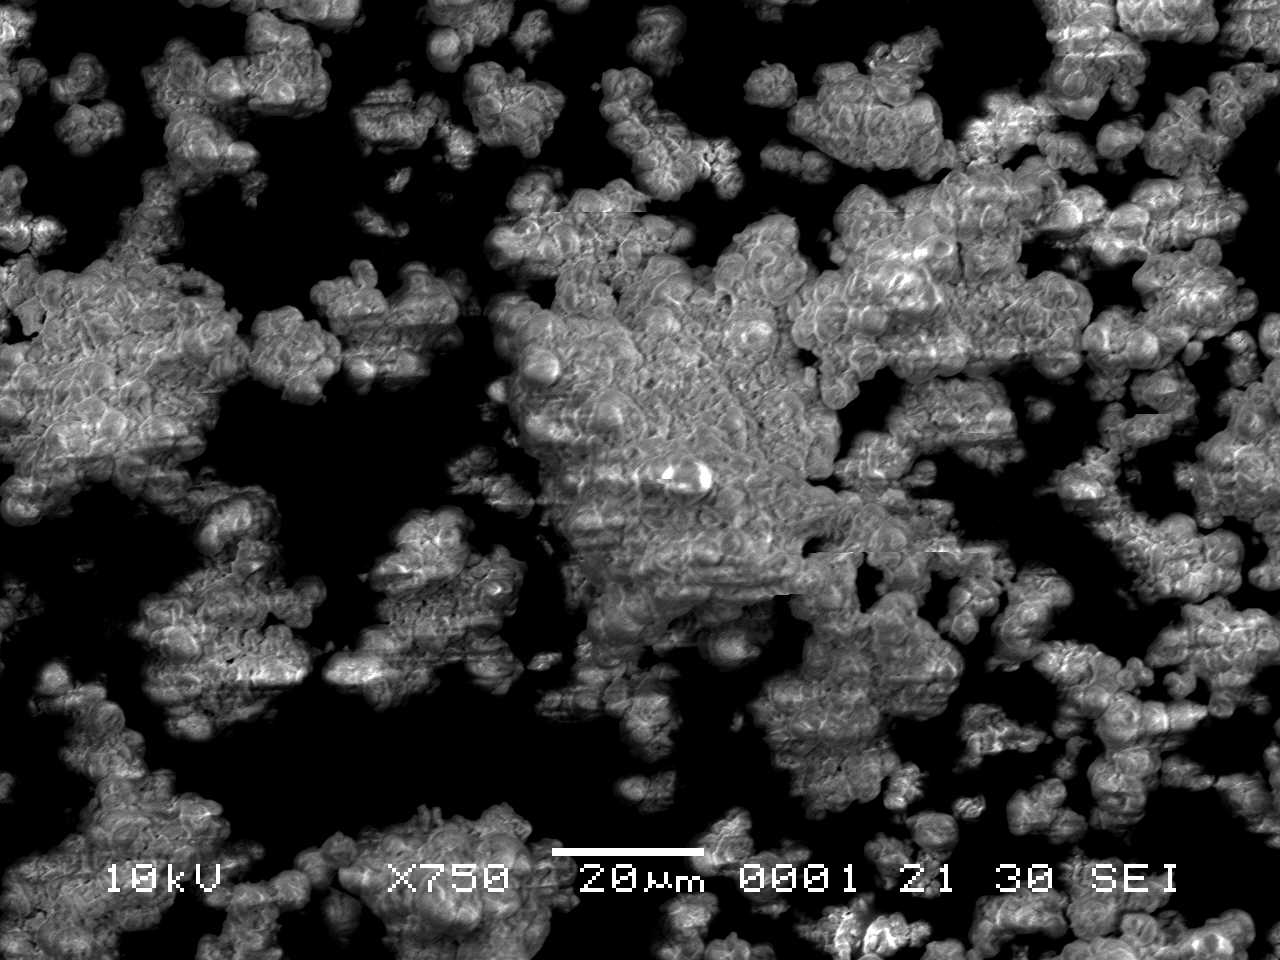
\includegraphics[width=\linewidth]{Fitz1_x750_1_030321}
\end{minipage}
\caption[SEM images: Sample Fitz1, blue verditer]{SEM images: Sample Fitz1, blue verditer. Magnification: \textbf{left)} 250x, \textbf{right)} 750x}
\label{fig:Fitz1_sem_1}
\end{figure}

At 1500x magnification (\textit{Figure \ref{fig:Fitz1_sem_2}}, left), there are clearly spherical particles. These have formed aggregates, though it is not clear whether individual particles could be separated back out of the larger clusters. The size is similar to the spherical cluster in the AzOp sample. The surface also looks slightly pocked or porous. 

The image shown at 2500x magnification (\textit{Figure \ref{fig:Fitz1_sem_2}}, right) is of lower quality than that at 1500x due to surface charging and jumping which made slower acquisitions unsuccessful. The faster acquisition does appear to flatten the image somewhat, which is important to consider since this makes it difficult to judge the volume of particles. There appear to be relatively flat aggregations of approximately circular particles with diameters of approximately 5 $\mu$m.

\begin{figure}[H]
\centering
\begin{minipage}{.45\textwidth}
  \centering
  \includegraphics[width=\linewidth]{Fitz1_x1500_2_030321}
\end{minipage}
\begin{minipage}{.45\textwidth}
  \centering
  \includegraphics[width=\linewidth]{Fitz1_x2500_1_030321}
\end{minipage}
\caption[SEM images: Sample Fitz1, blue verditer]{SEM images: Sample Fitz1, blue verditer. Magnification: \textbf{left)} 1500x, \textbf{right)} 2500x}
\label{fig:Fitz1_sem_2}
\end{figure}

% ************************************************     KE3     *******************************************************************

\textit{Figures \ref{fig:KE3_sem_1}} and \textit{Figure \ref{fig:KE3_sem_2}} show sample KE3 at magnifications from 250x to 2000x. The sample is described as light verditer bice. Verditer suggests a synthetic origin, while bice is used to refer to both natural and synthetic blue pigments. Tentatively, this sample is assumed to be synthetic based on this information.

The image collected at 250x magnification (\textit{Figure \ref{fig:KE3_sem_1}}, left) showed minor issues with charging. Very small particles are present with minimal aggregation. These appear very uniform in size and slightly spherical. At 750x magnification (\textit{Figure \ref{fig:KE3_sem_1}}, right), the uniformity of the particles is more easily observed. They are fairly symmetric, but more angular than sample Fitz1. There are some areas of needle-like structures as well as stacks of spherical or octagonal particles forming small aggregates.

\begin{figure}[H]
\centering
\begin{minipage}{.45\textwidth}
  \centering
  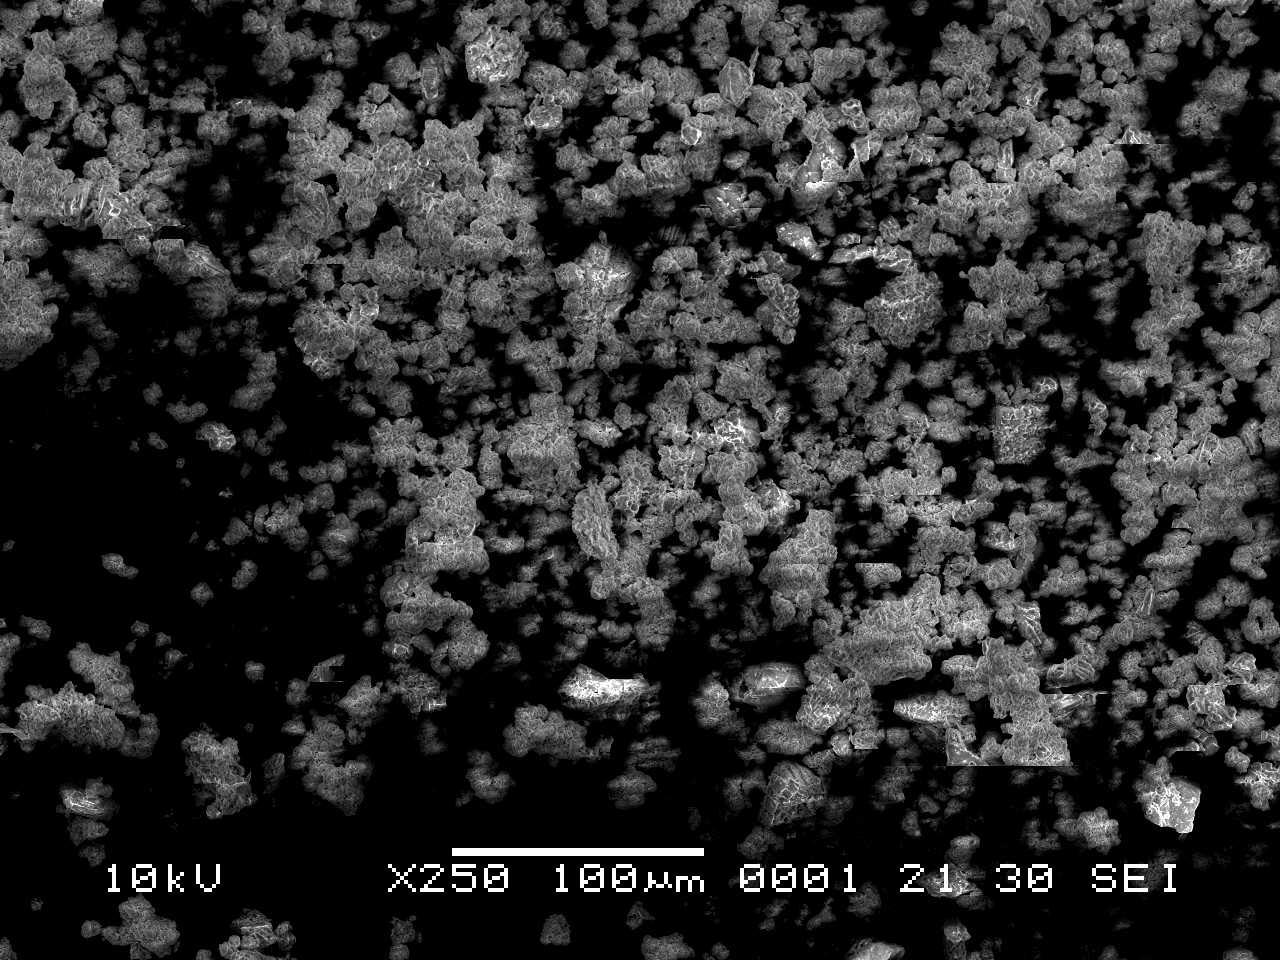
\includegraphics[width=\linewidth]{KE3_x250_1_050321}
\end{minipage}
\begin{minipage}{.45\textwidth}
  \centering
  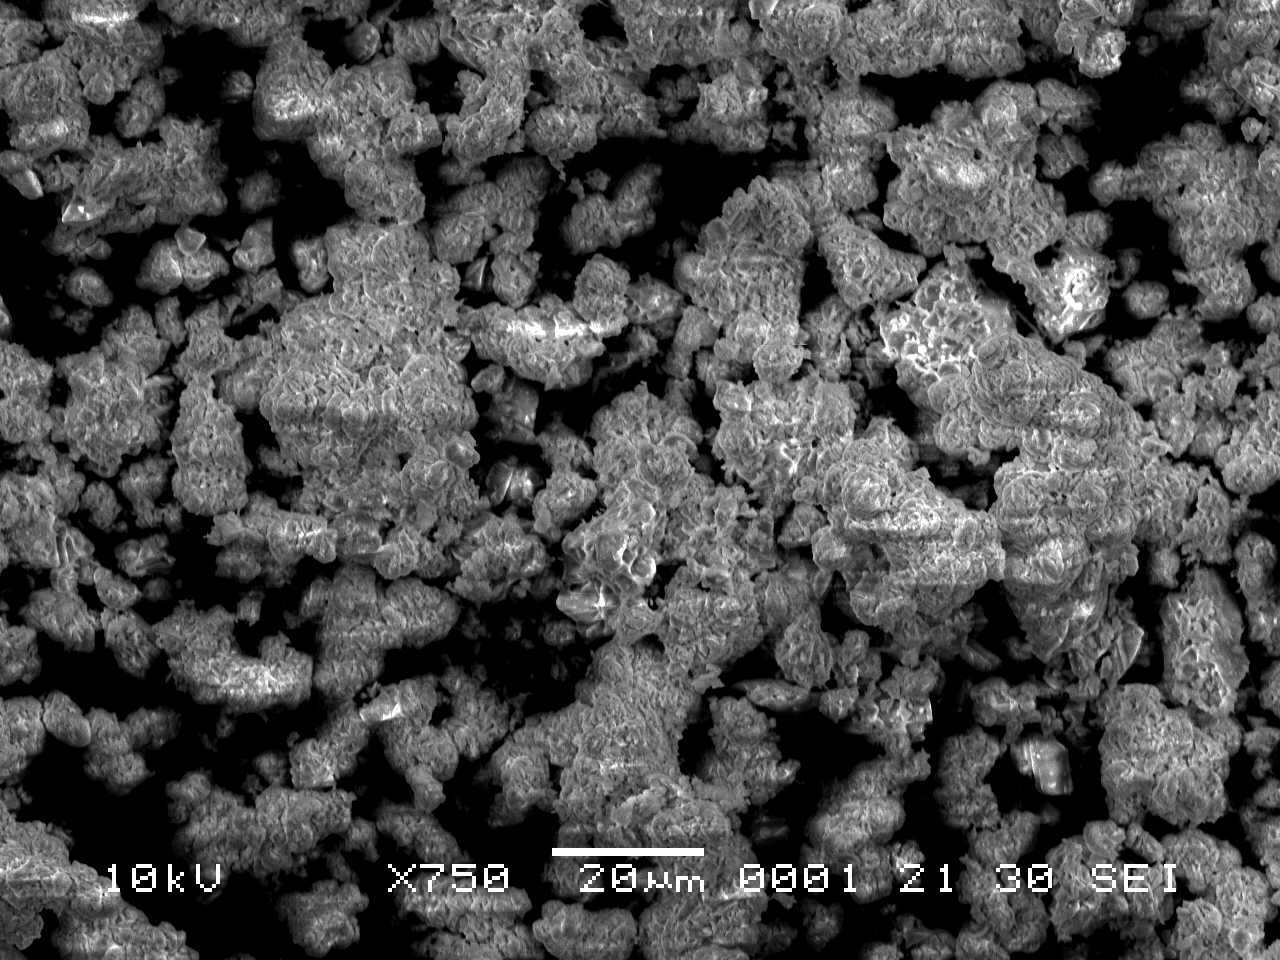
\includegraphics[width=\linewidth]{KE3_x750_3_050321}
\end{minipage}
\caption[SEM images: Sample KE3, light verditer bice]{SEM images: Sample KE3, light verditer bice. Magnification: \textbf{left)} 250x, \textbf{right)} 750x}
\label{fig:KE3_sem_1}
\end{figure}

The approximate particle size can be approximated to 5-10 $\mu$m from the image collected at 1500x magnification (\textit{Figure \ref{fig:KE3_sem_2}}, left). The surfaces appear more porous or pocked than sample Fitz1, but particles are more spherical and uniform than samples from natural origin. At 2000x magnification (\textit{Figure \ref{fig:KE3_sem_2}}, right), spheres are observed. There is significant texture on the surface that is quite fine especially around the edges of particles, and this texture appears rougher than that of sample Fitz1. This may be due, though, to poorer image quality of the Fitz1 sample.

\begin{figure}[H]
\centering
\begin{minipage}{.45\textwidth}
  \centering
  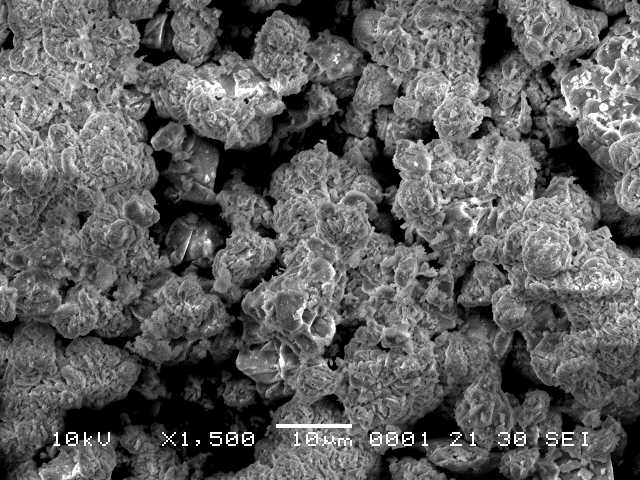
\includegraphics[width=\linewidth]{KE3_x1500_1_050321}
\end{minipage}
\begin{minipage}{.45\textwidth}
  \centering
  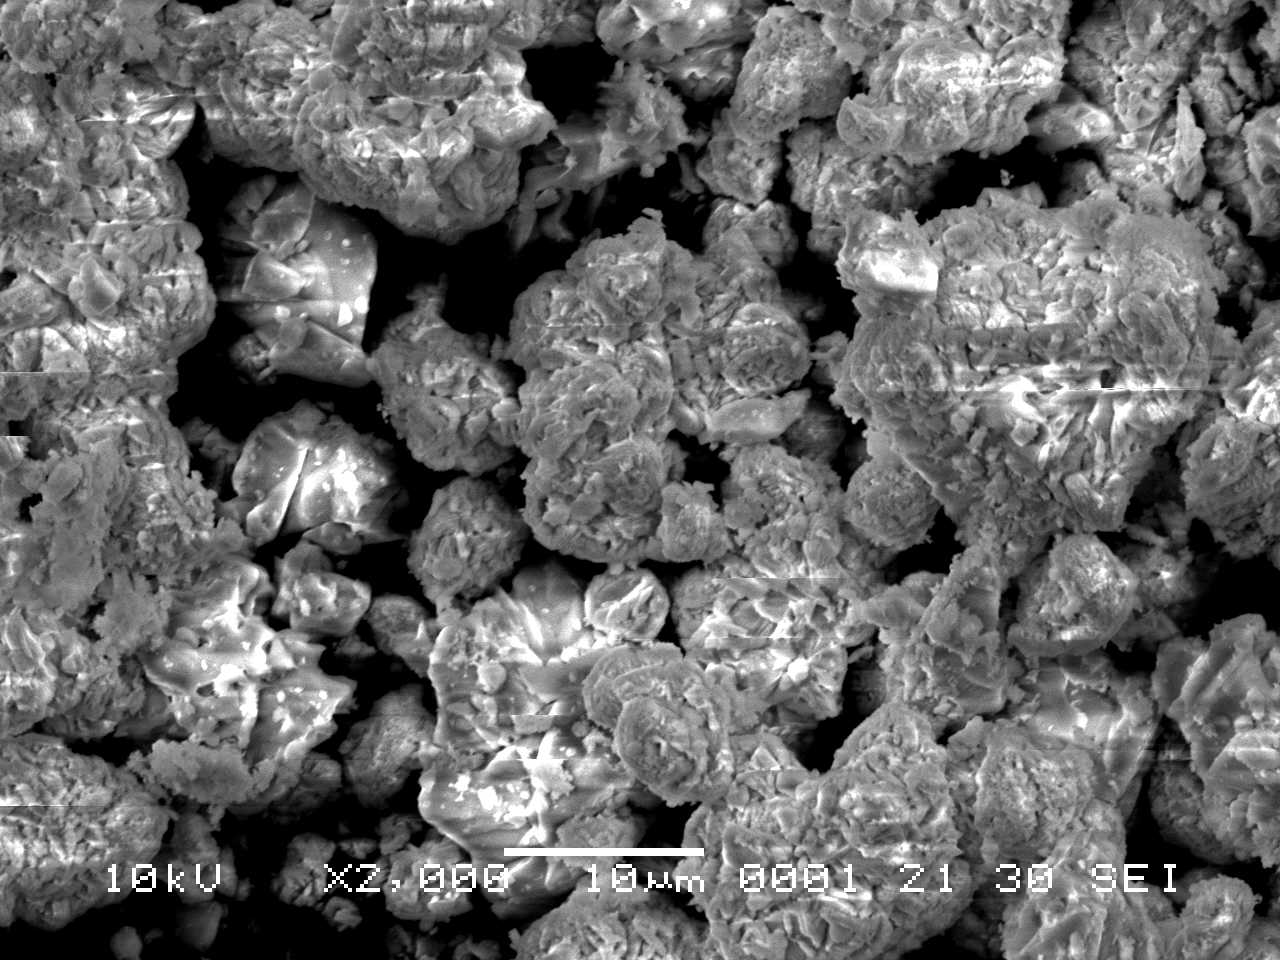
\includegraphics[width=\linewidth]{KE3_x2000_2_050321}
\end{minipage}
\caption[SEM images: Sample KE3, light verditer bice]{SEM images: Sample KE3, light verditer bice. Magnification: \textbf{left)} 1500x, \textbf{right)} 2000x}
\label{fig:KE3_sem_2}
\end{figure}

% ************************************************     KE4     *******************************************************************

\textit{Figures \ref{fig:KE4_sem_1}} and \textit{Figure \ref{fig:KE4_sem_2}} show sample KE4 at magnifications from 250x to 2000x. KE4 is labelled as blue bice, which is an ambiguous description, so it is inconclusive whether this sample was prepared naturally or synthetically.

\textit{Figure \ref{fig:KE4_sem_1}} (left) shows KE4 at 250x magnification. Larger particles on the order of 50 $\mu$m are visible, as are significantly smaller particles on the order of 5 $\mu$m. At 750x magnification (\textit{Figure \ref{fig:KE4_sem_1}}, right), fine needle-like structure is visible similar to that of sample HKI natural azurite. At the same time, there are also rounder structures that resemble Fitz1. 

\begin{figure}[H]
\centering
\begin{minipage}{.45\textwidth}
  \centering
  \includegraphics[width=\linewidth]{KE4_x250_1_030321}
\end{minipage}
\begin{minipage}{.45\textwidth}
  \centering
  \includegraphics[width=\linewidth]{KE4_x750_1_030321}
\end{minipage}
\caption[SEM images: Sample KE4, blue bice]{SEM images: Sample KE4, blue bice. Magnification: \textbf{left)} 250x, \textbf{right)} 750x}
\label{fig:KE4_sem_1}
\end{figure}

\textit{Figure \ref{fig:KE4_sem_2}} (left) shows KE4 at 1000x magnification, where the fine structure resembling needles or feathers is very clear. These structures are not oriented in any way, and appear randomly assembled. \textit{Figure \ref{fig:KE4_sem_2}} (right) shows KE4 at 2000x magnification. The image is focused on the flat side of a larger particle (or aggregate) with many smaller particles attached to or resting on the surface. There are also pockmarks or cavities observed. This sample is ambiguous as it shows characteristics of known natural as well as synthetic samples.

\begin{figure}[H]
\centering
\begin{minipage}{.45\textwidth}
  \centering
  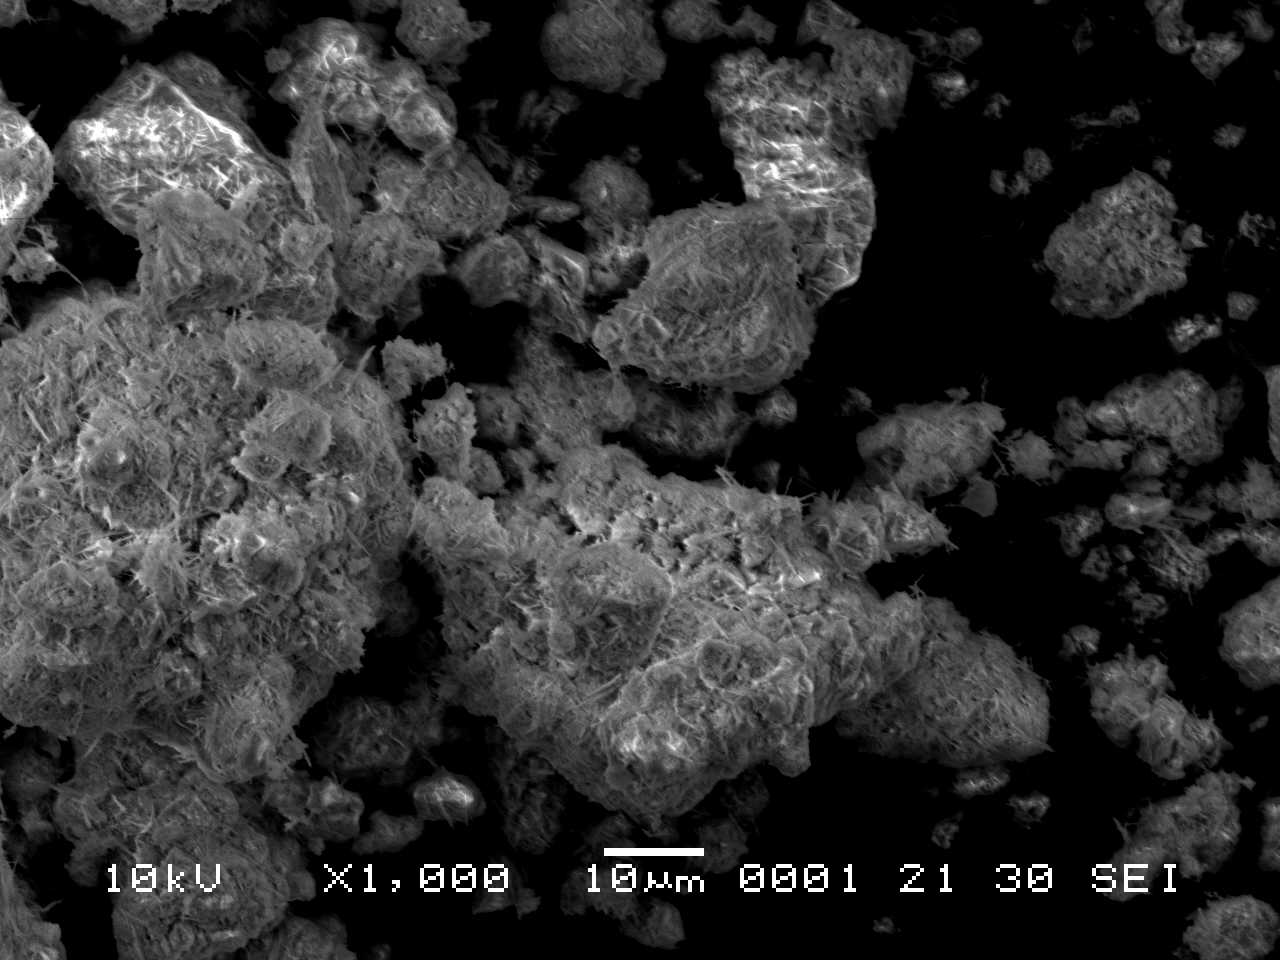
\includegraphics[width=\linewidth]{KE4_x1000_1_030321}
\end{minipage}
\begin{minipage}{.45\textwidth}
  \centering
  \includegraphics[width=\linewidth]{KE4_x2000_1_030321}
\end{minipage}
\caption[SEM images: Sample KE4, blue bice]{SEM images: Sample KE4, blue bice. Magnification: \textbf{left)} 1000x, \textbf{right)} 2000x}
\label{fig:KE4_sem_2}
\end{figure}

% ************************************************     KE5     *******************************************************************

\textit{Figures \ref{fig:KE5_sem_1}} and \textit{Figure \ref{fig:KE5_sem_2}} show sample KE5 at magnifications from 250x to 2000x. KE5 is described as blue verditer, strongly suggesting a synthetic origin.

\textit{Figure \ref{fig:KE5_sem_1}} (left) shows KE5 at 250x magnification. Small circular particles of uniform size and shape are observed. \textit{Figure \ref{fig:KE5_sem_1}} (right) shows KE5 at 750x magnification. At this magnification, larger aggregates of approximately 80 $\mu$m are clearly seen to be formed from smaller particles. This is very similar to the appearance of Fitz1 at the same magnification. The appearance also brings to mind the crystal formation of desert rose gypsum, characterized by intersecting flat discs forming circular or semicircular three dimensional structures.%~\autocite{hope_gypsum} 

\textit{Figure \ref{fig:KE5_sem_2}} shows KE5 at 1500x magnification (left) and 2000x magnification (right). The circular character of particles is very clearly observed in these images.

\begin{figure}[H]
\centering
\begin{minipage}{.45\textwidth}
  \centering
  \includegraphics[width=\linewidth]{KE5_x250_2_050321}
\end{minipage}
\begin{minipage}{.45\textwidth}
  \centering
  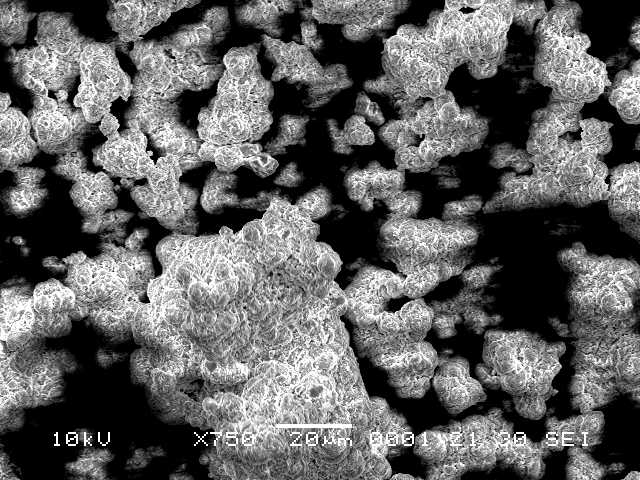
\includegraphics[width=\linewidth]{KE5_x750_1_050321}
\end{minipage}
\caption[SEM images: Sample KE5, blue verditer]{SEM images: Sample KE5, blue verditer. Magnification: \textbf{left)} 250x, \textbf{right)} 750x}
\label{fig:KE5_sem_1}
\end{figure}

\begin{figure}[H]
\centering
\begin{minipage}{.45\textwidth}
  \centering
  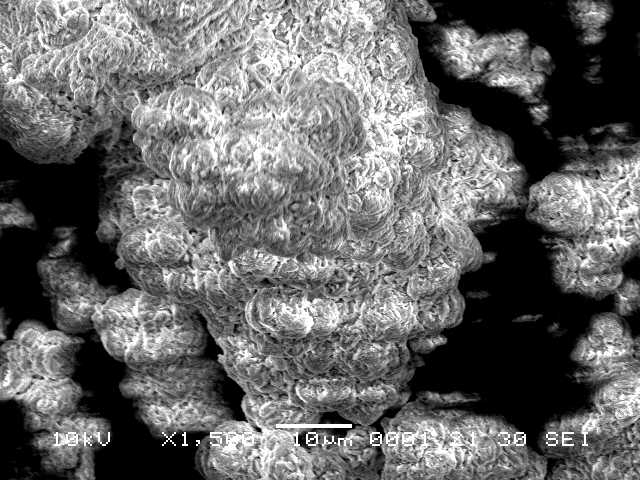
\includegraphics[width=\linewidth]{KE5_x1500_1_050321}
\end{minipage}
\begin{minipage}{.45\textwidth}
  \centering
  \includegraphics[width=\linewidth]{KE5_x2000_2_050321}
\end{minipage}
\caption[SEM images: Sample KE5, blue verditer]{SEM images: Sample KE5, blue verditer. Magnification: \textbf{left)} 1500x, \textbf{right)} 2000x}
\label{fig:KE5_sem_2}
\end{figure}

\subsubsection[Particle size distribution of natural and artificial azurite]{Particle size distribution of natural and artificial azurite}
\label{subsubsection3.1.1.1}

SEM images at 750x magnification were collected from edges of loose pigments samples used for SEM analysis above where particles were most loosely dispersed. The two powder samples selected, HKI natural azurite and Fitz 1, were selected on the basis of their known sources as well as significantly different morphology. The historical cross section was also analysed using the same method. These images were processed in ImageJ (Version 1.53a) by increasing contrast and manually thresholding (shown in \textit{Figures \ref{imageJ_fitz1} and \ref{fig:imageJ_hki}}) followed by manual selection of maximum lengths and measurement using the image scale bar. 

Five images of Fitz 1 were analysed, with n(particles) = 102. Five images of HKI natural azurite were analysed, with n(particles) = 127. Three images of the historical cross section were analysed, with n(particles) = 153. There is undoubtedly some bias in selected particles due to the difficulty of defining edges in the images, and this may affect the spread of results. Examples of the original SEM image (left) and the thresholded binary image (right, used for measurements) are shown for Fitz 1 in \textit{Figure \ref{fig:imageJ_fitz1}} and for HKI natural azurite in \textit{Figure \ref{fig:imageJ_hki}}. 

\begin{figure}[H]
\centering
\begin{minipage}{.45\textwidth}
  \centering
  \includegraphics[width=\linewidth]{Fitz1_x750_5_130521}
\end{minipage}
\begin{minipage}{.45\textwidth}
  \centering
  \includegraphics[width=\linewidth]{Fitz1_x750_5_130521_BW}
\end{minipage}
\caption[Particle size analysis: Sample Fitz 1]{Particle size analysis: Sample Fitz 1. \textbf{Left)} original SEM image, \textbf{Right)} thresholded binary image.}
\label{fig:imageJ_fitz1}
\end{figure}

\begin{figure}[H]
\centering
\begin{minipage}{.45\textwidth}
  \centering
  \includegraphics[width=\linewidth]{HKI_natural_azurite_x750_1_130521}
\end{minipage}
\begin{minipage}{.45\textwidth}
  \centering
  \includegraphics[width=\linewidth]{HKI_natural_azurite_x750_1_130521-2_BW}
\end{minipage}
\caption[Particle size analysis: Sample HKI natural azurite]{Particle size analysis: Sample HKI natural azurite. \textbf{Left)} original SEM image, \textbf{Right)} thresholded binary image.}
\label{fig:imageJ_hki}
\end{figure}

The measurements from each sample image were combined and analysed using R (RStudio Version 1.3.1093) to produce a histogram of the frequency of length measurements (bin size = 1 $\mu$m) for each sample, shown in \textit{Figure \ref{fig:histogram_length}}. Based on the different particle morphologies, it would be reasonable to expect that the particle size distribution would differ between samples. Additionally, the presence of a bimodal distribution in the histogram might indicate the formation of aggregates of a specific size from single particles. 

The length distributions of Fitz 1 and HKI natural azurite do not show significant differences. Both show a high frequency of particles with lengths around 5 $\mu$m, with a low frequency of particles or clusters above 10 $\mu$m. Sample Fitz 1 does appear to have several particles of length around 15 $\mu$m, which is absent in HKI natural azurite. This could suggest that aggregates are forming at more consistent sizes than in sample HKI natural azurite. Overall, though, these two samples are statistically very similar in this analysis. \textit{Table \ref{table:r_stats}} contains descriptive statistics, and it is notable how similar the means (and to some extent medians) are between all three samples. There is a notably larger range of particle lengths in the natural azurite sample, though this may be an artifact of processing since the historical cross section shows overall smaller particle sizes than both powder samples. 

\begin{figure}[H]
\centering
\begin{minipage}{.45\textwidth}
  \centering
  \includegraphics[width=\linewidth]{hist_fitz1}
\end{minipage}
\begin{minipage}{.45\textwidth}
  \centering
  \includegraphics[width=\linewidth]{hist_hki}
\end{minipage}
\caption[Particle size analysis: HKI natural azurite, Fitz 1]{Particle size analysis: Sample HKI natural azurite. \textbf{Left)} Fitz 1, \textbf{Right)} HKI natural azurite.}
\label{fig:histogram_length}
\end{figure}

\begin{figure}[H]
\centering
  \includegraphics[width=0.9\linewidth]{hist_xsection}
\caption[Particle size analysis: historical cross section]{Particle size analysis: historical cross section.} 
\label{fig:hist_xsec}
\end{figure}

\begin{table}[H]
\caption{Descriptive statistics: Fitz 1, HKI natural azurite, historical cross section}
\centering
\label{table:r_stats}
\begin{tabular}{c c c c}
\toprule
Reference sample & Mean & Median & Range \\
\midrule
HKI natural azurite & 8.583 & 5.437 & 1.177 - 52.176 \\
Fitz 1 & 8.683 & 5.878 & 2.414 - 38.367 \\
Historical cross section & 8.328 & 7.648 & 2.142 - 28.930 \\
\bottomrule
\end{tabular}
\end{table}

Lengths of the three samples are compared side-by-side in \textit{Figure \ref{fig:hist_all}}. The effect of outliers on the mean values of particle sizes is apparent, since both powder samples (black, red) show length distributions that, apart from a few larger outliers, are located at smaller lengths than that of the cross section in spite of all three datasets having very similar mean values. 

The difference between the powder samples and the cross section may be due to a number of factors. The preparation of pigments likely differed in the 15th century as compared to today, though azurite's optical properties depend on the size of its particle grains and we may therefore expect the fineness of grinding not to vary wildly. 

The suspension in a binding medium would be expected to affect the dispersion of grains, and this could reasonably affect aggregation (whether or not it would hinder aggregation depends on the hydrophilicity of the mineral, which is low in the case of azurite).~\autocite{Zhang} Optimal dispersion may also be orientation dependent. As discussed above, sampling bias will be present as only the x and y dimensions of the grains can be measured using this method, and depending on the orientation of particles relative to the slicing of the cross section, certain orientations may be over or underrepresented. 

The preparation of the cross section by resin embedding followed by microtoning will affect the appearance of particles under SEM. Microtoning may visually flatten the particles, making it difficult to see smaller grains. 

\begin{figure}[H]
\centering
  \includegraphics[width=0.9\linewidth]{hist_fitz1_hki_xsec_largerange}
\caption[Particle size analysis: HKI natural azurite, Fitz 1, historical cross section]{Particle size analysis: Fitz 1 (black), HKI natural azurite (red), historical cross section (blue).} 
\label{fig:hist_all}
\end{figure}


%fitz 1
%Median : 5.878  
%Mean   : 8.683
%range 2.414 to 38.367
% hki 
%Median : 5.437  
%Mean   : 8.583
%range 1.177 to 52.176

% *******************************************************************************************************************************
% *******************************************************************************************************************************
% *******************************************************************************************************************************

\subsection[Malachite and green verditer]{Malachite and green verditer}
\label{subsection3.1.2}

% ************************************************     Ma1     *******************************************************************

\textit{Figures \ref{fig:Ma1_sem_1}-\ref{fig:Ma1_sem_4}} show sample Ma1 at magnifications from 250x to 4000x. This sample is natural malachite.

At low magnification (200-250x) as shown in \textit{Figure \ref{fig:Ma1_sem_1}}, the sample appears extremely powdery and fine. The size and shape of particles are extremely irregular in both size and shape. 

\begin{figure}[H]
\centering
\begin{minipage}{.45\textwidth}
  \centering
  \includegraphics[width=\linewidth]{Ma1_x200_1_240221}
\end{minipage}
\begin{minipage}{.45\textwidth}
  \centering
  \includegraphics[width=\linewidth]{Ma1_x250_2_160321}
\end{minipage}
\caption[SEM images: Sample Ma1, malachite]{SEM images: Sample Ma1, malachite. Magnification: \textbf{left)} 200x, \textbf{right)} 250x}
\label{fig:Ma1_sem_1}
\end{figure}

At 750x magnification (\textit{Figure \ref{fig:Ma1_sem_2}}, left), the extreme irregularity of particles is apparent. Particles have extremely rough and choppy edges, and these irregular shapes closely resemble those of natural azurite samples in terms of their roughness and sharpness. There are few aggregates or clumps that are larger than 20 $\mu$m. At 1500x magnification (\textit{Figure \ref{fig:Ma1_sem_2}}, right), the texture of surfaces of the large (approx. 20 $\mu$m) aggregates is observed. It consists of particles of less than 5 $\mu$m across. 
\begin{figure}[H]
\centering
\begin{minipage}{.45\textwidth}
  \centering
  \includegraphics[width=\linewidth]{Ma1_x750_2_160321}
\end{minipage}
\begin{minipage}{.45\textwidth}
  \centering
  \includegraphics[width=\linewidth]{Ma1_x1500_2_160321}
\end{minipage}
\caption[SEM images: Sample Ma1, malachite]{SEM images: Sample Ma1, malachite. Magnification: \textbf{left)} 750x, \textbf{right)} 1500x}
\label{fig:Ma1_sem_2}
\end{figure}

\textit{Figure \ref{fig:Ma1_sem_3}} shows two areas of the sample at 2500x magnification. The sample is disordered and heterogeneous. While it is possible that this is due to grinding the pigment during preparation, \textit{Figure \ref{fig:Ma1_sem_4}} shows further disorder at 3000x and 4000x magnification. Here, many particles under 1 $\mu$m across are present, with extremely uneven borders. These are unambiguously single particles rather than surface roughness on a larger plane.


\begin{figure}[H]
\centering
\begin{minipage}{.45\textwidth}
  \centering
  \includegraphics[width=\linewidth]{Ma1_x2500_2_160321}
\end{minipage}
\begin{minipage}{.45\textwidth}
  \centering
  \includegraphics[width=\linewidth]{Ma1_x2500_3_160321}
\end{minipage}
\caption[SEM images: Sample Ma1, malachite]{SEM images: Sample Ma1, malachite. Magnification: 2500x}
\label{fig:Ma1_sem_3}
\end{figure}

\begin{figure}[H]
\centering
\begin{minipage}{.45\textwidth}
  \centering
  \includegraphics[width=\linewidth]{Ma1_x3000_2_160321}
\end{minipage}
\begin{minipage}{.45\textwidth}
  \centering
  \includegraphics[width=\linewidth]{Ma1_x4000_1_160321}
\end{minipage}
\caption[SEM images: Sample Ma1, malachite]{SEM images: Sample Ma1, malachite. Magnification: \textbf{left)} 3000x, \textbf{right)} 4000x}
\label{fig:Ma1_sem_4}
\end{figure}

% ************************************************     KE1a     *******************************************************************

\textit{Figures \ref{fig:KE1a_sem_1}} shows sample KE1a at magnifications 250x (left) and 750x (right). The name of Ke1a, green bice, is ambiguous and could refer to a natural or an artificial sample.

At 250x magnification, small particles form aggregations of approximately 25-50 $\mu$m. The image at 750x magnification is poor quality, and charging prevented use of higher magnifications. The shapes of particles do appear to be squared-off circles with some degree of uniformity. \mynote{(there may be a better way to say this)} They are not, however, spherical like several of the blue pigment samples discussed above. 

This sample is qualitatively more uniform than sample Ma1, and more spherical, but it is more challenging to draw clear conclusions about morphological differences between natural and synthetic green samples compared to blue. There is a much smaller sample size in the reference samples available, as well as ambiguity in sample source, but this also may just mean that green samples do not show marked morphology changes depending on production process.

\begin{figure}[H]
\centering
\begin{minipage}{.45\textwidth}
  \centering
  \includegraphics[width=\linewidth]{KE1a_x250_1_040321}
\end{minipage}
\begin{minipage}{.45\textwidth}
  \centering
  \includegraphics[width=\linewidth]{KE1a_x750_2_040321}
\end{minipage}
\caption[SEM images: Sample KE1a, green bice]{SEM images: Sample KE1a, green bice. Magnification: \textbf{left)} 250x, \textbf{right)} 750x}
\label{fig:KE1a_sem_1}
\end{figure}

% ************************************************     KE1b     *******************************************************************

%didnt do this one

% ************************************************     KE2     *******************************************************************

\textit{Figures \ref{fig:KE2_sem_1}} and \textit{\ref{fig:KE2_sem_2}} show sample KE2, green verditer. The sample name strongly suggests a synthetic source. 

In \textit{Figure \ref{fig:KE2_sem_1}}, the sample is shown at 250x (left) and 750x (right) magnifications. At 250x magnification, the sample appears fairly uniform in size and shape. It is very finely ground or naturally consists of small crystals and aggregates. At 750x magnification, particles are very irregularly shaped, sharp, and generally not elongated.

\begin{figure}[H]
\centering
\begin{minipage}{.45\textwidth}
  \centering
  \includegraphics[width=\linewidth]{KE2_250_1_040321}
\end{minipage}
\begin{minipage}{.45\textwidth}
  \centering
  \includegraphics[width=\linewidth]{KE2_x750_1_040321}
\end{minipage}
\caption[SEM images: Sample KE2, green verditer]{SEM images: Sample KE2, green verditer. Magnification: \textbf{left)} 250x, \textbf{right)} 750x}
\label{fig:KE2_sem_1}
\end{figure}

In \textit{Figure \ref{fig:KE2_sem_2}}, the sample is shown at 1500x (left) and 2000x (right) magnifications. It is possible to estimate the particle size at approximately 7-10 $\mu$m in the image at 1500x magnification. At 2000x magnification, there is a lack of texture on the surface of individual particles. The edges of particles are extremely feathery, which is observed in other samples discussed in this section as well.

\begin{figure}[H]
\centering
\begin{minipage}{.45\textwidth}
  \centering
  \includegraphics[width=\linewidth]{KE2_x1500_040321}
\end{minipage}
\begin{minipage}{.45\textwidth}
  \centering
  \includegraphics[width=\linewidth]{Ke2_x2000_1_040321}
\end{minipage}
\caption[SEM images: Sample KE2, green verditer]{SEM images: Sample KE2, green verditer. Magnification: \textbf{left)} 1500x, \textbf{right)} 2000x}
\label{fig:KE2_sem_2}
\end{figure}

\subsection[Historical samples]{Historical samples}
\label{subsection3.1.3}

SEM images of a historical cross section removed from a 15th c. old masters work (XXXX specifics) are presented.

Images were collected on two different instruments, XXXX and XXXX. The sample was coated with 24 nm carbon to decrease charging. On the Jeol SEM, images were collected using the backscatter electron detector (BES) which is sensitive to the atomic weight of the elements present in the sample: heavier elements will appear lighter in BES images. The BES detector was used in low vacuum mode to prevent sample charging. On the XXXX SEM, images were collected using the secondary electron detector (SE) and the BES detector simultaneously. 

\textit{Figures \ref{fig:xsection_jeol_1}}-\textit{\ref{fig:xsection_jeol_3}} show the cross section at low magnification (550-750x). The entire width of the cross section is shown, and three distinct layers are visible. The sample contains natural azurite and artificial blue verditer pigment particles, as well as other pigments that are not copper based and, presumably, some form of organic binder in which the pigment particles are embedded. Thin cracks can be seen dividing the pigment layers as well as through the entire cross section vertically. \textit{Figure \ref{fig:hki_crossec_explanation}} labels these three layers A, B, C, with C containing, per the intensity of the BES image, relatively lower atomic weight components. 

The size and shape of pigment particles is extremely uneven. The medium grey pigment in layers A and B is copper based according to EDX results (discussed in next section). EDX results also allow assignment of the bright white particles and aggregates to lead, likely a lead carbonate based on the presence of oxygen and absence of chromium (a component of lead yellow) as well as the color of the cross section under magnification. The copper based particles are morphologically distinct from the lead and manganese (darkest) particles, with dimensions on the order of 10-20 $\mu$m. Discussion of the copper containing pigments follows.

\textit{Figures \ref{fig:xsection_jeol_4}}-\textit{\ref{fig:xsection_jeol_7}} show the cross section at high magnification (1400-2500x) using the Jeol instrument, and \textit{Figures \ref{fig:xsection_dept_1}}-\textit{\ref{fig:xsection_dept_8}} show the cross section at 1000x to 12,500x magnification using the XXXX instrument. The Jeol instrument in BES shows much more apparent contrast between different elements than the XXXX instrument, and this makes it slightly more straightforward to interpret. The XXXX instrument, on the other hand, shows both BES (left) and SE (right) images and offers much sharper resolution but allows poor distinguishing between pigments without the use of mapping. In \textit{Figure \ref{fig:xsection_dept_1}} and others, images capture the structure of the bound cross section clearly, with areas of pitting and cracking visible. One feature that is not easily explained is the feathery, indistinctly bound areas of white in the BES images. As this feature is not present in the SE images, it is not explained by surface charging. Morphologically, it looks to be due to an organic layer of binder, embedding resin, or carbon coating (????) rather than due to any pigment.

At higher magnification, the irregularity of orientation and shape of particles is clear. \textit{Figure \ref{fig:xsection_dept_8}} shows the sample at high magnification in an area where copper blue pigments are expected to be present. Here, interesting planar morphology is shown which resembles that of samples Az 1 and AzMag (see \textit{Figures \ref{fig:az1_sem_2}} and \textit{\ref{fig:azmag_sem_5}}).

\mynote{This is confusing!}

\begin{figure}[H]
\centering
  \includegraphics[width=0.9\linewidth]{hki_crossec_explanation}
\caption[Historical cross section with visually distinct layers A, B, and C labelled]{Historical cross section, SEM image at 550x magnification, with visually distinct layers A, B, and C labelled.}
\label{fig:hki_crossec_explanation}
\end{figure}

\begin{figure}[H]
\centering
\begin{minipage}{.45\textwidth}
  \centering
  \includegraphics[width=\linewidth]{hki_xsection_BES_LV_x550_40spot_250621}
\end{minipage}
\begin{minipage}{.45\textwidth}
  \centering
  \includegraphics[width=\linewidth]{hki_xsection_BES_LV_x550_58spot_240621}
\end{minipage}
\caption[SEM images: Historical cross section, azurite and blue verditer]{SEM images: Historical cross section, azurite and blue verditer. Magnification: 550x}
\label{fig:xsection_jeol_1}
\end{figure}

\begin{figure}[H]
\centering
\begin{minipage}{.45\textwidth}
  \centering
  \includegraphics[width=\linewidth]{hki_xsection_BES_LV_x750_2_58spot_240621}
\end{minipage}
\begin{minipage}{.45\textwidth}
  \centering
  \includegraphics[width=\linewidth]{hki_xsection_BES_LV_x750_3_58spot_240621}
\end{minipage}
\caption[SEM images: Historical cross section, azurite and blue verditer]{SEM images: Historical cross section, azurite and blue verditer. Magnification: 750x}
\label{fig:xsection_jeol_2}
\end{figure}

\begin{figure}[H]
\centering
\begin{minipage}{.45\textwidth}
  \centering
  \includegraphics[width=\linewidth]{hki_xsection_BES_LV_x750_58spot_240621}
\end{minipage}
\begin{minipage}{.45\textwidth}
  \centering
  \includegraphics[width=\linewidth]{hki_xsection_x750_2_250621}
\end{minipage}
\caption[SEM images: Historical cross section, azurite and blue verditer]{SEM images: Historical cross section, azurite and blue verditer. Magnification: 750x. Right image is collected using the secondary electron (SE) detector.}
\label{fig:xsection_jeol_3}
\end{figure}

\begin{figure}[H]
\centering
\begin{minipage}{.45\textwidth}
  \centering
  \includegraphics[width=\linewidth]{hki_xsection_x1400_2_250621}
\end{minipage}
\begin{minipage}{.45\textwidth}
  \centering
  \includegraphics[width=\linewidth]{hki_xsection_BES_LV_x1500_3_40spot_250621}
\end{minipage}
\caption[SEM images: Historical cross section, azurite and blue verditer]{SEM images: Historical cross section, azurite and blue verditer. Magnification: \textbf{left)} SE detector: 1400x, \textbf{right)} 1500x}
\label{fig:xsection_jeol_4}
\end{figure}

\begin{figure}[H]
\centering
\begin{minipage}{.45\textwidth}
  \centering
  \includegraphics[width=\linewidth]{hki_xsection_BES_LV_x1500_40spot_250621}
\end{minipage}
\begin{minipage}{.45\textwidth}
  \centering
  \includegraphics[width=\linewidth]{hki_xsection_BES_LV_x1500_2_40spot_250621}
\end{minipage}
\caption[SEM images: Historical cross section, azurite and blue verditer]{SEM images: Historical cross section, azurite and blue verditer. Magnification: 1500x}
\label{fig:xsection_jeol_5}
\end{figure}

\begin{figure}[H]
\centering
\begin{minipage}{.45\textwidth}
  \centering
  \includegraphics[width=\linewidth]{hki_xsection_BES_LV_x2300_2_40spot_250621}
\end{minipage}
\begin{minipage}{.45\textwidth}
  \centering
  \includegraphics[width=\linewidth]{hki_xsection_BES_LV_x2300_40spot_250621}
\end{minipage}
\caption[SEM images: Historical cross section, azurite and blue verditer]{SEM images: Historical cross section, azurite and blue verditer. Magnification: 2300x}
\label{fig:xsection_jeol_6}
\end{figure}

\begin{figure}[H]
\centering
\begin{minipage}{.45\textwidth}
  \centering
  \includegraphics[width=\linewidth]{hki_xsection_BES_LV_x2500_2_40spot_250621}
\end{minipage}
\begin{minipage}{.45\textwidth}
  \centering
  \includegraphics[width=\linewidth]{hki_xsection_BES_LV_x2500_40spot_250621}
\end{minipage}
\caption[SEM images: Historical cross section, azurite and blue verditer]{SEM images: Historical cross section, azurite and blue verditer. Magnification: 2500x}
\label{fig:xsection_jeol_7}
\end{figure}


\begin{figure}[H]
\centering
  \includegraphics[width=0.9\linewidth]{hki_cross_section_img_290621_01}
\caption[SEM images: Historical cross section, azurite and blue verditer]{SEM images: Historical cross section, azurite and blue verditer. Magnification: 1000x}
\label{fig:xsection_dept_1}
\end{figure}

\begin{figure}[H]
\centering
  \includegraphics[width=0.9\linewidth]{hki_cross_section_img_290621_04}
\caption[SEM images: Historical cross section, azurite and blue verditer]{SEM images: Historical cross section, azurite and blue verditer. Magnification: 1500x}
\label{fig:xsection_dept_2}
\end{figure}

\begin{figure}[H]
\centering
  \includegraphics[width=0.9\linewidth]{hki_cross_section_img_290621_08}
\caption[SEM images: Historical cross section, azurite and blue verditer]{SEM images: Historical cross section, azurite and blue verditer. Magnification: 2000x}
\label{fig:xsection_dept_3}
\end{figure}

\begin{figure}[H]
\centering
  \includegraphics[width=0.9\linewidth]{hki_cross_section_img_290621_03}
\caption[SEM images: Historical cross section, azurite and blue verditer]{SEM images: Historical cross section, azurite and blue verditer. Magnification: 3500x}
\label{fig:xsection_dept_4}
\end{figure}

\begin{figure}[H]
\centering
  \includegraphics[width=0.9\linewidth]{hki_cross_section_img_290621_12}
\caption[SEM images: Historical cross section, azurite and blue verditer]{SEM images: Historical cross section, azurite and blue verditer. Magnification: 4300x}
\label{fig:xsection_dept_5}
\end{figure}

\begin{figure}[H]
\centering
  \includegraphics[width=0.9\linewidth]{hki_cross_section_img_290621_05}
\caption[SEM images: Historical cross section, azurite and blue verditer]{SEM images: Historical cross section, azurite and blue verditer. Magnification: 5500x}
\label{fig:xsection_dept_6}
\end{figure}

\begin{figure}[H]
\centering
  \includegraphics[width=0.9\linewidth]{hki_cross_section_img_290621_10}
\caption[SEM images: Historical cross section, azurite and blue verditer]{SEM images: Historical cross section, azurite and blue verditer. Magnification: 5500x}
\label{fig:xsection_dept_7}
\end{figure}

\begin{figure}[H]
\centering
  \includegraphics[width=0.9\linewidth]{hki_cross_section_img_290621_11}
\caption[SEM images: Historical cross section, azurite and blue verditer]{SEM images: Historical cross section, azurite and blue verditer. Magnification: 12,500x}
\label{fig:xsection_dept_8}
\end{figure}

%%%%%%%
%%%%%%%
%%%%%%%
%%%%%%%
%%%%%%%
%%%%%%%
%%%%%%%
%%%%%%%
%%%%%%%
%%%%%%%
%%%%%%%
%%%%%%%

\section[EDS Data]{EDS Data}
\label{section3.2}

From the chemical formulas for azurite and malachite, it is possible to determine the expected ratios of elements detected by electron dispersive X-ray spectroscopy (EDS or EDX). Malachite (Cu\textsubscript{2}CO\textsubscript{3}(OH)\textsubscript{2}) has an expected Cu:O ratio of 2:5 or 0.4, while azurite (Cu\textsubscript{3}(CO\textsubscript{3})\textsubscript{2}(OH)\textsubscript{2}) has an expected Cu:O ratio of 3:8 or 0.375. Given an expected instrumental variation in oxygen detection of up to 10\%, it is difficult to distinguish between these two chemical formulas, but detection of Cu:O ratios within a small margin of error would allow confirmation of samples as basic copper carbonates.

Detection of other elements and mapping of element intensities can suggest other minerals present in samples. \textit{Table \ref{table:eds_elems}} shows elements detected in EDS analysis of reference samples and which samples contain which elements, based on collection of point spectra as well as mapping. Not all elements are detected at each point, though copper, oxygen, and carbon are detected in all samples. Carbon is additionally present in the instrument chamber as well as on the tab holding the pressed powder samples, and the quantitative percent carbon detected is therefore not used for analysis. Additionally, one historical sample, a cross section removed from a 16th c. old masters work(XXXX specifcis in lab) has been studied. This sample is significantly more complex, containing not only both natural azurite and synthetic blue verditer but also other pigment and binder components.

\begin{table}[H]
\caption{Reference sample descriptions}
\centering
\label{table:eds_elems}
\begin{tabular}{c c}
\toprule
Element & Detected in samples \\
\midrule
Carbon & Instrument, all samples \\
Oxygen & All samples \\
Copper & All samples \\
Silicon & Az1, Az2, AzMag, AzOp, HKI, Fitz1, historical cross section \\
Aluminium & Az1, AzOp, HKI, historical cross section \\
Magnesium & HKI, historical cross section \\
Calcium & AzMag, HKI, Fitz1, KE3, KE4, KE1a, historical cross section \\
Potassium & HKI, historical cross section \\
Iron & HKI, historical cross section \\
Lead & historical cross section (non-azurite component) \\
Arsenic & historical cross section (mapping only) \\
\bottomrule
\end{tabular}
\end{table}

Quantitative atomic ratios are presented for each sample in the same order as above for SEM images, and mapping data is presented where relevant. Individual point spectra with sample locations are provided in the appendix containing supplemental data \mynote{not yet}. One point spectrum with sample location is shown here as an example.

% ************************************************    HKI    ********************************************************************

\textit{Figures \ref{fig:hki_eds_spec}} and \textit{\ref{fig:hki_eds_semimage}} show an example EDS point spectrum collected from the sample HKI natural azurite and the corresponding sample location on the SEM image. Elements detected in the sample are C, O, Cu, Al, Si, K, Mg, and Fe. \textit{Table \ref{table:hki_ratios}} presents the quantitative Cu:O and Si:O ratios for eight sample locations. The Si:Al ratio is relatively constant with an average value of 1.42 across all samples, but the other atomic ratios show significant variation, suggesting a mixture of several mineral components.

\begin{figure}[H]
\centering
  \includegraphics[width=0.9\linewidth]{HKI_nat_az_EDS_site2_spectrum1_050521_spectrumimage}
\label{fig:hki_eds_spec}
\end{figure}

\begin{figure}[H]
\centering
  \includegraphics[width=0.9\linewidth]{HKI_nat_az_EDS_site2_spectrum1_050521_semimage}
\label{fig:hki_eds_semimage}
\end{figure}

\begin{table}[H]
\caption{HKI natural azurite: EDS quantitative data}
\centering
\label{table:hki_ratios}
\begin{tabular}{c c}
\toprule
\multicolumn{2}{c}{HKI natural azurite} \\
\midrule
Cu:O & Si:O \\
\midrule
0.0104 & 0.2152 \\
0.2558 & 0.0465 \\
0.0114 & 0.2906 \\
0.0040 & 0.1816 \\
0.3498 & 0.1667 \\
0.0251 & 0.3351  \\
0.0097 & 0.2499 \\
0.0060 & 0.1696 \\
\bottomrule
\end{tabular}
\end{table}

EDS mapping data is shown in \textit{Figures \ref{fig:hki_map1}} and \textit{\ref{fig:hki_map2}}. This shows that copper and oxygen abundance is highly correlated, and that Cu intensity makes up only approximately 50\% of the mapped area. Carbon distribution appears random, as does potassium and magnesium. Iron is present in only the first map (\textit{Figure \ref{fig:hki_map1}}) and appears correlated with oxygen, suggesting the presence of some form of iron oxide in low abundance. 

Silicon is correlated to both oxygen and aluminium in most areas in which it is present, with one area on the first map showing a silicon/oxygen containing compound that lacks aluminium. There is no apparent link between SEM morphology and elemental composition, and smaller surface particles are not elementally distinct from the larger substrate they rest on. Interestingly, the sample consists of as much or more copper-free content as copper-containing content, and only one of eight point spectra shows the expected Cu:O atomic ratio. 

\begin{figure}[H]
\centering
  \includegraphics[width=0.9\linewidth]{HKI_nat_az_EDS_map1_050521_imgs}
\label{fig:hki_map1}
\end{figure}

\begin{figure}[H]
\centering
  \includegraphics[width=0.9\linewidth]{HKI_nat_az_EDS_site3_map2_060521_imgs}
\label{fig:hki_map2}
\end{figure}

% ************************************************    Az1    ********************************************************************

C, O, Cu, Al, and Si were detected in sample Az 1. \textit{Table \ref{table:az1_ratios}} shows calculated Cu:O atomic ratios from point spectra. The average Cu:O ratio value is 0.3031 (SD = 0.0631). This is on the lower end of expected ratio values for azurite, though several ratio values are very close to that expected. The Si:O ratios were very consistent, averaging around 0.04, and the average Si:Al ratios were also quite consistent, averaging 1.44, though silicon was not present in all point spectra.

\begin{table}[H]
\caption{Az 1: EDS quantitative data}
\centering
\label{table:az1_ratios}
\begin{tabular}{c}
\toprule
Az 1, azurite \\
\midrule
Cu:O \\
\midrule
0.3150 \\
0.3236 \\
0.2920 \\
0.2018 \\
0.3969 \\
0.2893 \\
\bottomrule
\end{tabular}
\end{table}

\textit{Figures \ref{fig:az1_map1} - \ref{fig:az1_map3}} show mapping data for sample Az 1. Copper and oxygen are spatially correlated. Detection of zinc in one map is taken to be a false attribution and actually indicate copper due to overlapped peaks. Carbon is loosely correlated to copper and oxygen in \textit{Figure \ref{fig:az1_map3}}, but is clearly appearing in areas where the EDS carbon-basedf tab is exposed in all maps.

Discussion of silicon, aluminium, and oxygen is more complicated. \textit{Figure \ref{fig:az1_map1}} shows that aluminium and silicon both appear in the same areas as both copper and oxygen, which is unexpected. \textit{Figure \ref{fig:az1_map2}} and \textit{Figure \ref{fig:az1_map3}} show correlation of silicon with aluminium broadly and with oxygen in a few areas of high intensity.

\begin{figure}[H]
\centering
  \includegraphics[width=0.9\linewidth]{Az1_EDS_map1_250221_imgs}
\label{fig:az1_map1}
\end{figure}

\begin{figure}[H]
\centering
  \includegraphics[width=0.9\linewidth]{Az1_EDS_map2_250221_imgs}
\label{fig:az1_map2}
\end{figure}

\begin{figure}[H]
\centering
  \includegraphics[width=0.9\linewidth]{Az1_EDS_map3_250221_imgs}
\label{fig:az1_map3}
\end{figure}

% ************************************************    Az2    ********************************************************************

C, O, Cu, and Si were detected in sample Az 2. Cu:O ratios calculated from point spectra show inconsistent values, 0.2699 and 0.3897 (\textit{Table \ref{table:az2_ratios}}). However, the calculated Si:O ratios at the same locations do not explain the fluctuation; the ratio of 0.0198 Si:O is far too small to indicate a silicon oxide type mineral.

\begin{table}[H]
\caption{Az 2: EDS quantitative data}
\centering
\label{table:az2_ratios}
\begin{tabular}{c c}
\toprule
\multicolumn{2}{c}{Az 2, azurite} \\
\midrule
Cu:O & Si:O \\
\midrule
0.2699 & 0.0198 \\
0.3897 & 0 \\
\bottomrule
\end{tabular}
\end{table}

\textit{Figure \ref{fig:az2_map1}} shows that while copper and oxygen are highly correlated across the sample map, silicon and carbon are randomly distributed. This suggests that silicon is present as a trace element rather than a major component of the pigment, and this is supported by the low Si:O ratios calculated from the point spectra. This means that the variation in Cu:O atomic ratio values must be due to a factor other than intensity due to another mineral present.

\begin{figure}[H]
\centering
  \includegraphics[width=0.9\linewidth]{Az2_EDS_map1_250221_imgs}
\label{fig:az2_map1}
\end{figure}

% ************************************************    AzMag    ********************************************************************

The elements detected in sample AzMag are C, O, Cu, Si, and Ca. The calculated Cu:O ratios, shown in \textit{Table \ref{table:azmag_ratios}}, are 0.1786 and 0.3404. These are not consistent: 0.3404 is very close to the expected ratio for basic copper carbonates, but 0.1786 is well outside the expected range. Silicon is present at very low levels (approximate Si:O ratio = 0.01), and does not explain this variation. Calcium is present in the first sample with a ratio of 0.1012, which is significant. It is possible that a calcium containing mineral is present throughout this sample, a conclusion supported by mapping data.

\begin{table}[H]
\caption{AzMag: EDS quantitative data}
\centering
\label{table:azmag_ratios}
\begin{tabular}{c }
\toprule
AzMag, azurite \\
\midrule
Cu:O \\
\midrule
0.1786 \\
0.3404 \\
\bottomrule
\end{tabular}
\end{table}

\textit{Figure \ref{fig:azmag_map1}} shows mapping data for sample AzMag. Silicon and carbon show lower intensity than copper and oxygen, but all four are closely correlated spatially. Calcium was not detected in the mapping data.

\begin{figure}[H]
\centering
  \includegraphics[width=0.9\linewidth]{AzMag_EDS_map1_260221_imgs}
\label{fig:azmag_map1}
\end{figure}


% ************************************************    AzOp    ********************************************************************

C, O, Cu, Al, and Si are detected in sample AzOp. Atomic ratios are shown in \textit{Table \ref{table:azop_ratios}}. Cu:O ratios calculated from point spectra are very low in sample AzOp, while those of Si:Al and Si:O are relatively high compared to other samples. This suggests that the sample contains other minerals such as quartz or aluminum silicate may be present, though the calculated atomic ratios do not fit empirical formulae so it is not possible to allow determination of these minerals from EDS data alone.

\begin{table}[H]
\caption{AzOp: EDS quantitative data}
\centering
\label{table:azop_ratios}
\begin{tabular}{c c c}
\toprule
\multicolumn{3}{c}{AzOp, azurite} \\
\midrule
Cu:O & Si:Al & Si:O \\
\midrule
0.2330 & 1.2572 & 0.1051 \\
0.2062 & 1.1140 & 0.0753 \\
\bottomrule
\end{tabular}
\end{table}

\textit{Figure \ref{fig:azop_map1}} shows mapping data for sample AzOp. Copper and oxygen are clearly correlated, and carbon is somewhat correlated to copper and oxygen; all expected for a basic copper carbonate. However, areas also show significant correlation between silicon and oxygen. Silicon is abundant all over the sample. Mapping data does not show aluminium intensity, surprisingly. 

\begin{figure}[H]
\centering
  \includegraphics[width=0.9\linewidth]{AzOp_EDS_map1_260221_imgs}
\label{fig:azop_map1}
\end{figure}

% ************************************************    Fitz1    ********************************************************************

C, O, Cu, Al (mapping only), Si, and Ca were detected in sample Fitz 1. Atomic ratios are shown in \textit{Table \ref{table:fitz1_ratios}}. Given that Fitz 1 is a synthetic pigment, it is reasonable to hypothesize that it would contain only carbon, copper, and oxygen and show fairly consistent Cu:O ratios across point spectra. Surprisingly, low levels of silicon and calcium were detected, and Cu:O ratios range from 0.1366 (well below the expected ratio for a basic copper carbonate) to 0.3314 (approximately the expected ratio for a basic copper carbonate). Furthermore, the chemical variation is interesting when compared to the morphological consistency observed.

\begin{table}[H]
\caption{Fitz 1: EDS quantitative data}
\centering
\label{table:fitz1_ratios}
\begin{tabular}{c c c}
\toprule
\multicolumn{3}{c}{Fitz 1, blue verditer} \\
\midrule
Cu:O & Ca:O & Si:O \\
\midrule
0.2316 & 0.1555 & 0 \\
0.3115 & 0 & 0.0122 \\
0.1366 & 0.2510 & 0 \\
0.3314 & 0 & 0.0085 \\
\bottomrule
\end{tabular}
\end{table}

\textit{Figures \ref{fig:fitz1_map1}} and \textit{\ref{fig:fitz1_map2}} show mapping data for sample Fitz 1. Copper is spatially correlated with some areas of oxygen intensity, as is carbon. Calcium appears randomly distributed all over the mapped area. Silicon appears with oxygen in several spots with very high intensity, and aluminium and silicon also appear correlated.

\begin{figure}[H]
\centering
  \includegraphics[width=0.9\linewidth]{Fitz1_EDS_map1_020321_imgs}
\label{fig:fitz1_map1}
\end{figure}

\begin{figure}[H]
\centering
  \includegraphics[width=0.9\linewidth]{Fitz1_EDS_map1_030321_imgs}
\label{fig:fitz1_map2}
\end{figure}

% ************************************************    KE3    ********************************************************************

The elements detected in sample KE 3 are C, O, Cu, Ca, and Si (mapping only). \textit{Table \ref{table:ke3_ratios}} shows the Cu:O and Ca:O ratios from point spectra. While the first ratio value for Cu:O is as expected for a basic copper carbonate, the second is much lower and outside the expected range. This correlates with a much larger Ca:O ratio, suggesting that some particles in the sample may be calcium oxide rather than copper carbonate.

\begin{table}[H]
\caption{KE 3: EDS quantitative data}
\centering
\label{table:ke3_ratios}
\begin{tabular}{c c}
\toprule
\multicolumn{2}{c}{KE 3, light verditer bice} \\
\midrule
Cu:O & Ca:O \\
\midrule
0.3411 & 0.0069 \\
0.2052 & 0.1108 \\
\bottomrule
\end{tabular}
\end{table}

\textit{Figure \ref{ke3_map1}} shows mapping data for sample KE 3. Silicon appears in mapping data sporadically but not in point spectra. Copper is correlated with oxygen, as is calcium to some extent.

\begin{figure}[H]
\centering
  \includegraphics[width=0.9\linewidth]{KE3_EDS_map1_050321_imgs}
\label{fig:ke3_map1}
\end{figure}

% ************************************************    KE4    ********************************************************************

C, O, Cu, and Ca were detected in sample KE 4. Point spectra show calculated Cu:O ratios (\textit{Table \ref{table:ke4_ratios}}) that, while slightly low, are within range of that expected for azurite (particularly the second ratio, 0.3381). The calculated Ca:O ratios are very low.

\begin{table}[H]
\caption{KE 4: EDS quantitative data}
\centering
\label{table:ke4_ratios}
\begin{tabular}{c c}
\toprule
\multicolumn{2}{c}{KE 4, blue bice} \\
\midrule
Cu:O & Ca:O \\
\midrule
0.2703 & 0.0660 \\
0.3381 & 0.0095 \\
\bottomrule
\end{tabular}
\end{table}

\textit{Figure \ref{fig:ke4_map1}} shows mapping data for sample KE 4. Copper and oxygen, as observed in other samples, are spatially correlated. Carbon is also correlated to copper and oxygen. Calcium is correlated to oxygen as well, only in areas absent of copper, suggesting some form of calcium oxide is present.

\begin{figure}[H]
\centering
  \includegraphics[width=0.9\linewidth]{KE4_EDS_map1_030321_imgs}
\label{fig:ke4_map1}
\end{figure}

% ************************************************    KE5    ********************************************************************

The elements detected in sample KE 5 are C, O, and Cu. The average ratio of Cu:O is 0.3150, and all sampled atomic ratios are shown in \textit{Table \ref{table:ke5_ratios}}. While this value is lower than expected, it is within reason given the possible error in quantitative determination of oxygen.

\begin{table}[H]
\caption{KE 5: EDS quantitative data}
\centering
\label{table:ke5_ratios}
\begin{tabular}{c}
\toprule
KE 5, blue verditer \\
\midrule
Cu:O \\
\midrule
0.3371 \\
0.3284 \\
0.2794 \\
\bottomrule
\end{tabular}
\end{table}

% ************************************************    Ma1    ********************************************************************

The elements detected in sample Ma 1 are C, O, and Cu. \textit{Figure \ref{fig:ma1_map1}} shows mapping data from sample Ma 1. Zinc is also shown at low abundance in mapping data, though this is likely intensity due to copper since the peaks of copper and zinc overlap. There is correlation between carbon, oxygen, and copper, and the Cu:O ratio is 0.3675, expected for a basic copper carbonate compound. 

\begin{figure}[H]
\centering
  \includegraphics[width=0.9\linewidth]{Ma1_EDS_map1_250221_imgs}
\label{fig:ma1_map1}
\end{figure}

% ************************************************    KE1a    ********************************************************************

C, O, Cu, and Ca were detected in sample KE 1a. Calcium is present in relatively low levels, and is likely a trace element rather than a major component of the pigment. The measured Cu:O ratios (\textit{Table \ref{table:ke1a_ratios}}) are within the range expected for a basic copper carbonate.

\begin{table}[H]
\caption{KE 1a: EDS quantitative data}
\centering
\label{table:ke1a_ratios}
\begin{tabular}{c c}
\toprule
\multicolumn{2}{c}{KE 1a, green bice} \\
\midrule
Cu:O & Ca:O \\
\midrule
0.3483 & 0.0086 \\
0.3622 & 0.0066 \\
\bottomrule
\end{tabular}
\end{table}

% ************************************************    KE2    ********************************************************************

C, O, Cu, and Si (mapping only) were detected in sample KE 2. The measured Cu:O ratios (\textit{Table \ref{table:ke2_ratios}} are within the range expected for a basic copper carbonate, and are among the highest measured of any samples.

\begin{table}[H]
\caption{KE 2: EDS quantitative data}
\centering
\label{table:ke2_ratios}
\begin{tabular}{c}
\toprule
KE 2, green verditer \\
\midrule
Cu:O \\
\midrule
0.3724 \\
0.3944 \\
\bottomrule
\end{tabular}
\end{table}

\textit{Figures \ref{ke2_map1}} and \textit{\ref{ke2_map2}} show mapping data for sample KE 2. Carbon is sparsely distributed, and there are areas without any elements detected. Silicon, which is not detected in point spectra, is present in low levels. Copper and oxygen are clearly correlated, as expected.

\begin{figure}[H]
\centering
  \includegraphics[width=0.9\linewidth]{KE2_ES_map1_040321_imgs}
\label{fig:ke2_map1}
\end{figure}

\begin{figure}[H]
\centering
  \includegraphics[width=0.9\linewidth]{KE2_EDS_map1_050321_imgs}
\label{fig:ke2_map2}
\end{figure}

All three green samples (Ma 1, KE 1a, and KE 2) show Cu:O atomic ratios that very closely match the expected ratios for both azurite and malachite. The chemical formula for green verditer is as yet unproven, and the margin of error on quantitative analysis is not able to distinguish between a 2:5 and a 3:8 Cu:O ratio. It is clear that there is minimal trace mineral present in all these samples, and that atomic ratios support identification as basic copper carbonates.

%       *****************************

The historical cross section is significantly more complex than the powder samples, both natural and synthetic. Mapping data for the cross section collected on both the Jeol and XXXX SEM-EDS instruments are presented in \textit{Figures \ref{fig:xsection_map1}}-\textit{\ref{fig:xsection_map1}}. Azurite and verditer pigments are only two components of the sample. The cross section consists of three visually distinct layers, but EDS mapping data shows that layers A and B (in \textit{Figure \ref{ig:hki_crossec_explanation}}) are chemically comparable. The visual difference is likely due to the higher intensity of lead containing components in layer B. 

This sample was carbon-coated prior to analysis, so carbon is present across the entire sample surface. Oxygen is also distributed across the entirety of the cross section, which is expected as many common pigments are metal carbonates or metal oxides and any organic binder components will also contain oxygen. Calcium, aluminium, and silicon are also detected over the entire area of the cross section, with some map data showing correlation between aluminum and silicon. It is likely that an aluminosilicate is present in association with one or more pigments. Calcium-based ground layers are commonly observed, and a material such as limestone could contain Ca, Si, and Al as well as potassium, also detected in the cross section. Potassium is observed in the natural azurite sample from the HKI, which might suggest it is also a marker that could be used to evaluate the nature of azurite pigments.

That said, there is also evidence that aluminosilicates are present as distinct components, as observed in \textit{Figure \ref{fig:xsection_map4}} where silicon and aluminium are observed to be present in precisely localised areas. Calcite is a common mineral associated with azurite and is observed in almost all powder samples, natural and artificial. Calcium carbonates as well as aluminosilicates including kaolinite were also both commonly used as paint extenders, white particles mixed with coloured pigments to lower their cost to produce.~\autocite{Townsend}

Magnesium, lead, and copper are localised to areas of the sample that correspond with distinct pigment particles or aggregates as discussed above. Given the lack of chromium present as well as the colour of the cross sectional layers, the lead pigment present is suggested to be lead white, a basic Lead(II) carbonate that occurs as a mineral called cerussite. While cerussite may occur in association with natural azurite,\autocite{Aru} the abundance of lead and the lack of overlapping areas of lead and copper detected by EDS suggests that lead white was employed as a pigment mixed with the blue azurite.

Magnesium oxides have been used historically as pigments, most importantly \textit{terre verte} or green earth which is a mixture of an iron silicate with a magnesium-containing clay. The low abundance of iron across the sample discourages the assignment of magnesium to terre verte, and therefore, magnesium-based minerals associated with azurite or cerussite must be considered as an explanation. Additionally, magnesium may be present as mica or another common mineral. Iron is detected sporadically across the cross section, which suggests that it is present as a trace element. Arsenic is suggested in one EDS map (\textit{Figure \ref{HKI_cross_section_Site 7_2021-06-30_15-23-55}}), and this must be evaluated further.

Quantitative analysis of copper containing areas of the sample shows a Cu:O ratio of, on average, 0.217. This is lower than the expected ratio for azurite/blue verditer. Also detected in these areas are significant levels of iron and lead, indicating that there may be impurities in the blue pigment particles (iron) and/or contribution from the three dimensional structure of the paint mixture containing azurite and lead white. At lower levels there is also silicon and magnesium detected, which may be due to impurities as well. 

This data demonstrates the complexity of analysis of samples consisting of a mixture of different pigments that are also each composed of, potentially, several minerals.

%O, Cu, Ca, Pb, Mg, Al, Si, K, Fe ( map only: As??)

%Darkest: Mg on mapping (low atomic number)
%Lightest: Lead, fine powder, widely distributed through one of the laters, likely mixed with Cu to make a lighter color (lead white)
%Moderate: Copper
%Darker layer shows relatively more Si in mapping

\begin{figure}[H]
\centering
  \includegraphics[width=0.9\linewidth]{hki_xsection_eds_260621_map1_x700}
\label{fig:xsection_map1}
\end{figure}

\begin{figure}[H]
\centering
  \includegraphics[width=0.9\linewidth]{hki_cross_section_eds_analysis_250621_site1_map1}
\label{fig:xsection_map2}
\end{figure}

\begin{figure}[H]
\centering
  \includegraphics[width=0.9\linewidth]{hki_xsection_eds_260621_map2_x2300}
\label{fig:xsection_map3}
\end{figure}

\begin{figure}[H]
\centering
  \includegraphics[width=0.9\linewidth]{hki_xsection_eds_260621_map3_x2300}
\label{fig:xsection_map4}
\end{figure}

\begin{figure}[H]
\centering
  \includegraphics[width=0.9\linewidth]{hki_xsection_eds_260621_map4_x2300}
\label{fig:xsection_map5}
\end{figure}

\textit{Figures \ref{fig:xsection_map6}} and \textit{\ref{fig:xsection_map7}} show mapping data collected from a more sensitive EDS instrument (is this fair?). The magnification is approximately 2000x here.

\begin{figure}[H]
\centering
  \includegraphics[width=0.9\linewidth]{HKI_cross_section_Site 1_2021-06-30_15-15-34}
\label{fig:xsection_map6}
\end{figure}

\begin{figure}[H]
\centering
  \includegraphics[width=0.9\linewidth]{HKI_cross_section_Site 7_2021-06-30_15-23-55}
\label{fig:xsection_map7}
\end{figure}




% *******************************************************************************************************************************
% *******************************************************************************************************************************
% *******************************************************************************************************************************

\section[Raman Data]{Raman Data}
\label{section3.3}

\mynote{not done}

\textit{Figure \ref{fig:label_raman}} shows Raman spectra of samples Az1 (blue) and Ma1 (green). The spectrum from Az1 was collected from a bright blue particle, while the spectrum from Ma1 was collected from the fine green bulk particles. Both therefore are representative of the component of the pigment responsible for the colour rather than of another mineral impurity (which will be discussed further down). Peak centers are labelled.

Hydroxyl stretching bands are reported by Frost et. al. for azurite at 3453 and 3427 cm\textsuperscript{-1} and for malachite at 3468 and 3386 cm\textsuperscript{-1}.~\autocite{Frost} These bands are not shown here, but were observed. Mattei et. al. note that bands below 600 cm\textsuperscript{-1} are due to CuO vibrations and bands from 600 to 1600 cm\textsuperscript{-1} are due to carbonate vibrations.


azurite
Frost: $v1    v2_Sym  v2_Antisym   v3_B2   v3_A1    v4_B2   v4_A1$
       1095   816       834        1419    1430     765     739

Bicchieri: 145, 180, 250, 284, 335, 403, 545, 746, 767, 839, 940, 1098, 1432 and 1573 cm

Mattei: 157vw 174vw 182vw 240vw 250vw \textbf{267vw} 282vw 332vw
\textbf{387vw} 402s 542vw \textbf{744vw is shoulder} 768w 840w 937vw 1099m
1422m(sh) \textbf{1433m is shoulder in mine} 1462vw 1582w 3431w

Me: \textbf{113 139 migtht be too low or 139 might be 145} 180 248 284 330 401 \textbf{501} 541 \textbf{577} 764sh 836sh  937 1096 1419sh 1459 1576
Good agreement but I have two extra peaks (501, 577) and Mattei etal have extra 387, 267


malachite

mattei: \textbf{157m(sh) 171m(sh) 182s 204vw 224vw} 272s 352w 435s 513w
537m 601vw 723vw 753vw 1058w 1101w 1370vw 1463vw
1497s 3380w

frost: $v1    v2_Sym  v2_Antisym   v3_B2   v3_A1    v4_B2   v4_A1$
      1096     816      801       1492     1364     752     717
                                  1514     1423

me: 119 145(sh) 154 169(sh) 179 221 270 351 432 503 529 557 580 628 718 952 1005 1057 1096 1363 1492 1579 1595 1723
Not observed: 204 mattei, 537 mattei, 601 mattei, 752 (753 mattei), 801 816
537 and 601 are liekly convoluted with the complex peaks
me not seen elsewhere: 118, 145, [503 529 557 580 628], 952, 1005, 1579 1595 1723
do not fit quartz, chalconatrite, hoganite, 





\begin{figure}[H]
\centering
\begin{minipage}[t]{\linewidth}
  \centering
  \includegraphics[width=0.9\linewidth]{az1_blue_withlabels}
\hfill
\includegraphics[width=0.9\linewidth]{Ma1_labels_ACTUAL}
\hfill
\end{minipage}
\caption[Raman spectra of natural azurite and malachite, peak centers labelled.]{Raman spectra of natural azurite (blue, top) and malachite (green, bottom). Peak centers are labelled.}
\label{fig:label_raman}
\end{figure}
\mynote{rescale green in order to have same x range}

\begin{figure}[H]
\centering
  \includegraphics[width=0.9\linewidth]{blue_HKI_Az1_Az2_labels}
\label{fig:blue_comparison1}
\end{figure}

\begin{figure}[H]
  \centering
  \includegraphics[width=0.9\linewidth]{blue_HKI_AzMag_AzOp_Ke4}
\label{fig:blue_comparison2}
\end{figure}

\begin{figure}[H]
  \centering
  \includegraphics[width=0.9\linewidth]{blue_Fitz1_Ke5_Ke3_Ke4_labels_actual}
\caption[Raman spectra of blue samples, peak centers labelled.]{Raman spectra of natural azurite and synthetic blue verditer samples. Peak centers are labelled to highlight variations in spectra.}
\label{fig:blue_comparison3}
\end{figure}

\begin{figure}[H]
\centering
  \includegraphics[width=0.9\linewidth]{green_pigments_all_labels_ACTUAL.jpg}
\caption[Raman spectra of green samples, peak centers labelled.]{Raman spectra of natural malachite and synthetic green verditer samples. Peak centers are labelled to highlight variations in spectra.}
\label{fig:green_comparison}
\end{figure}

Analysis of resin embedded samples, including historical cross sections, proved difficult using the confocal Raman system. \textit{Figure \ref{fig:fluor_example_graph}} shows two spectra collected using an excitation wavelength of 532 nm from the surface of the historical cross section sample. Azurite is clearly present in one spectrum, shown in black, with a strong band at 400 cm\textsuperscript{-1} (band highlighted in blue). Cerussite (lead white) is present in both spectra (highlighted in grey). Broac baselines were subtracted but it is apparent from the presence of a regular scalloped peak shape that additional fluorescence is present. Analysis of the polyester resin without pigment present shows that these bands are from resin contributions, though similar fluorescense has also appeared as discussed previously in spectra of impurities in powdered azurite and verditer samples. 

These bands are present in all spectra collected from the historical cross section sample, and the signal is strong enough to mask contributions from smaller azurite peaks and is comparable in intensity to contributions from cerussite, a major component of the cross section along with azurite. This clearly poses a problem for detection of variation in pigments and introduces uncertainty into the results.

\textit{Figure \ref{fig:contours_xsection}} shows contour plots of azurite peak intensity (left) and integrated peak area (right) across a 10 x 10 spectrum map of an area of the cross section. The undertainty introduced by the strong resin bands is apparent, as peak area and peak intensity do not indicate azurite particles are present in the same areas of the map. This is due to varying contributions from the underlying fluorescence band that are difficult to subtract without introducing additional errors into the analysis.

\begin{figure}[H]
\centering
  \includegraphics[width=0.9\linewidth]{fluor_example_graph}
\caption[Raman spectra of historical cross section]{Raman spectra of two points on historical cross section, blue area. The semicircular repeated peak formation observed is due to fluorescence from the resin (contribution from non-azurite pigment particles and organic binder is also possible). The major azurite (blue) and cerussite (grey) peaks are highlighted on the graph and spectra are offset for clarity.}
\label{fig:fluor_example_graph}
\end{figure}


\begin{figure}[H]
\centering
\begin{minipage}{.45\textwidth}
  \centering
  \includegraphics[width=\linewidth]{050721map400intensities}
\end{minipage}
\begin{minipage}{.45\textwidth}
  \centering
  \includegraphics[width=\linewidth]{050721map400areas}
\end{minipage}
\caption[Contour maps, azurite Raman intensity in historical cross section]{Contour maps show the Raman intensity as: \textbf{left)} 400 cm\textsuperscript{-1} peak intensity and \textbf{right)} 400 cm\textsuperscript{-1} integrated peak area. X and Y axes map to locations on the sample surface where spectra were collected, in total 10 x 10 = 100 spectra.}
\label{fig:contours_xsection}
\end{figure}

The 473 nm excitation wavelength was also tested to determine whether the fluorescence would be mitigated by shifting the excitation frequency. This was determined not to resolve the issue, with fluorescence and sample bands showing a similar increase in intensity at 473 nm. It may be possible to generate sample spectra without fluorescence by moving to the anti-Stokes spectrum rather than the Stokes spectrum, as fluorescence is not possible in the anti-Stokes region. However, this may come at the cost of overall intensity and signal-to-noise strength.

%az1_blue_withlabels
%Ma1_labels

%green_pigments_all_labels
%blue_HKI_AzMag_AzOp_Ke4
%blue_HKI_Az1_Az2_labels
%blue_Fitz1_Ke5_Ke3_labels
%blue_Fitz1_Ke5_Ke3_Ke4_labels


% *******************************************************************************************************************************
% *******************************************************************************************************************************
% *******************************************************************************************************************************

\section[AFM Data]{AFM Data}
\label{section3.4}

%      HKI natural azurite

AFM images recorded in tapping mode capture height, deflection, and phase variation across the sample surface. While height measurements are self-explanatory, phase and deflection measurements record variations in mechanical and chemical properties that are not easily deconvoluted or quantified. Deflection refers to the displacement of the tip with interaction with the surface, while the phase shift refers to the difference between the oscillation frequency of the tip initially and after interaction with the surface.~\autocite{iscpi} The phase shift and deflection measurements are therefore affected by changes in the tip interaction with the surface such as adherence or repulsion. 

Height effects can also appear in phase and deflection maps, appearing as intensity changes that change direction as the tip passes over a structure on the surface of the sample. These will appear, for instance, as a high deflection voltage or phase shift on the left side of the structure and a low deflection voltage or phase shift on the right side as the tip scans from left to right. This is due to changing the contact area of the tip with the sample as it approaches a change in topography.~\autocite{iscpi} 



80x80 (3.59): The image quality isn’t great – there is some horizontal dragging. Small circular particles are seen. Overall, this image does not give too much information about the sample.
def 80x80 (3.59): Poor quality, looks like some instrument noise maybe. Waves.
phase 80x80 (3.60): Some quality issues, but the surface texture is dense and particles appear rounded. 


\begin{figure}[H]
\centering
\begin{minipage}{.45\textwidth}
  \centering
  \includegraphics[width=\linewidth]{hki_nataz_tapping_mode_150721_height_1}
\end{minipage}
\begin{minipage}{.45\textwidth}
  \centering
  \includegraphics[width=\linewidth]{hki_nataz_tapping_mode_150721_def_1}
\end{minipage}
\caption[Height and deflection maps, HKI natural azurite]{Height and deflection maps, HKI natural azurite, 80 x 80 $\mu$m.}
\label{fig:afm_hki_nataz_height_def_1}
\end{figure}

\begin{figure}[H]
\centering
  \includegraphics[width=.45\textwidth]{hki_nataz_tapping_mode_150721_phase_1}
\caption[Phase map, HKI natural azurite]{Phase map, HKI natural azurite, 80 x 80 $\mu$m.}
\label{fig:afm_hki_nataz_phase_1}
\end{figure}

40x40 (3.61): Fairly good quality image. Appears to be significant size variation, with some features up to 20 um across and 25 um tall, but I’m a bit suspect of how flat these structures are and deflection image raises questions about tip contact here.
def 40x40 (3.61): Poor image quality. Some horizontal dragging/noise, otherwise some waves.
phase 40x40 (3.62): Poor quality due to horizontal dragging, but the surface texture is visible in some places and looks to be fairly rough. (Guessing this is not compositional differences, but rather height differences…)


\begin{figure}[H]
\centering
\begin{minipage}{.45\textwidth}
  \centering
  \includegraphics[width=\linewidth]{hki_nataz_tapping_mode_150721_height_2}
\end{minipage}
\begin{minipage}{.45\textwidth}
  \centering
  \includegraphics[width=\linewidth]{hki_nataz_tapping_mode_150721_def_2}
\end{minipage}
\caption[Height and deflection maps, HKI natural azurite]{Height and deflection maps, HKI natural azurite, 40 x 40 $\mu$m.}
\label{fig:afm_hki_nataz_height_def_2}
\end{figure}

\begin{figure}[H]
\centering
  \includegraphics[width=.45\textwidth]{hki_nataz_tapping_mode_150721_phase_2}
\caption[Phase map, HKI natural azurite]{Phase map, HKI natural azurite, 40 x 40 $\mu$m.}
\label{fig:afm_hki_nataz_phase_2}
\end{figure}

15x15 (3.63): This image does show both large structures (<15 um) and very small spherical features.
def 15x15 (3.63): Poor image, horizontal dragging and concentric rings.
phase 15x15 (3.64): This image is poor quality with very significant horizontal dragging. Unfortunately this may show finer structure but it is difficult to determine this across whole image due to the dragging. 


\begin{figure}[H]
\centering
\begin{minipage}{.45\textwidth}
  \centering
  \includegraphics[width=\linewidth]{hki_nataz_tapping_mode_150721_height_3}
\end{minipage}
\begin{minipage}{.45\textwidth}
  \centering
  \includegraphics[width=\linewidth]{hki_nataz_tapping_mode_150721_def_3}
\end{minipage}
\caption[Height and deflection maps, HKI natural azurite]{Height and deflection maps, HKI natural azurite, 15 x 15 $\mu$m.}
\label{fig:afm_hki_nataz_height_def_3}
\end{figure}

\begin{figure}[H]
\centering
  \includegraphics[width=.45\textwidth]{hki_nataz_tapping_mode_150721_phase_3}
\caption[Phase map, HKI natural azurite]{Phase map, HKI natural azurite, 15 x 15 $\mu$m.}
\label{fig:afm_hki_nataz_phase_3}
\end{figure}

5x5 (3.65):  Despite some horizontal dragging, this image is relatively useable. The flat surface structure does seem to be a surface contact issue because significant texture is visible here. The smaller rounded areas don’t seem to be separate from the larger pieces for the most part. The larger pieces here are not remotely spherical and have dimensions of approximately 2x3 um up to 2x4 or 2x5 um.
def 5x5 (3.65): Poor image, concentric waves.
phase 5x5 (3.66): Horizontal pulling makes this image difficult to interpret. It does not appear to deviate from the height image. 

\begin{figure}[H]
\centering
\begin{minipage}{.45\textwidth}
  \centering
  \includegraphics[width=\linewidth]{hki_nataz_tapping_mode_150721_height_4}
\end{minipage}
\begin{minipage}{.45\textwidth}
  \centering
  \includegraphics[width=\linewidth]{hki_nataz_tapping_mode_150721_def_4}
\end{minipage}
\caption[Height and deflection maps, HKI natural azurite]{Height and deflection maps, HKI natural azurite, 5 x 5 $\mu$m.}
\label{fig:afm_hki_nataz_height_def_4}
\end{figure}

\begin{figure}[H]
\centering
  \includegraphics[width=.45\textwidth]{hki_nataz_tapping_mode_150721_phase_4}
\caption[Phase map, HKI natural azurite]{Phase map, HKI natural azurite, 5 x 5 $\mu$m.}
\label{fig:afm_hki_nataz_phase_4}
\end{figure}

40x40 (3.67): Odd looking image that almost looks vertically stretched. There are some tall spots that are very small and look rounded, but these look questionable based on them not appearing in any other image for this sample and generally.
def 40x40 (3.61): Poor image quality. Some horizontal dragging/noise, otherwise some waves.
phase 40x40 (3.68): This is a reasonable quality image. There may be some gain noise, and the strange rounded structures are still visible, but also some flat planes are observed. I am tempted to throw out this image. 


\begin{figure}[H]
\centering
\begin{minipage}{.45\textwidth}
  \centering
  \includegraphics[width=\linewidth]{hki_nataz_tapping_mode_150721_height_5}
\end{minipage}
\begin{minipage}{.45\textwidth}
  \centering
  \includegraphics[width=\linewidth]{hki_nataz_tapping_mode_150721_def_5}
\end{minipage}
\caption[Height and deflection maps, HKI natural azurite]{Height and deflection maps, HKI natural azurite, 40 x 40 $\mu$m.}
\label{fig:afm_hki_nataz_height_def_5}
\end{figure}

\begin{figure}[H]
\centering
  \includegraphics[width=.45\textwidth]{hki_nataz_tapping_mode_150721_phase_5}
\caption[Phase map, HKI natural azurite]{Phase map, HKI natural azurite, 40 x 40 $\mu$m.}
\label{fig:afm_hki_nataz_phase_5}
\end{figure}

%       Az 1

\textit{Figures \ref{1}}-\textit{\ref{2}} show height and deflection maps of 80 x 80 $\mu$m areas of sample Az 1. Height images show randomly oriented areas of higher topographies, which appear rounded and vary in size. It is possible that these structures arise from some clustering of smaller particles. This is consistent across all areas sampled. \textit{Figure \ref{3.67}, left} shows several pits of approximately 3-4 $\mu$m in depth, though the variation in finer features is approximately 750 nm. The boundary of the powder sample with the resin, shown in \textit{Figure \ref{3.71}, left}, is highly irregular. Macro scale aggregates range from 15 to 40 $\mu$m in size, with smaller spherical structures on top.

Deflection images from sample Az 1 are inconsistent. Several show concentric circles mapping approximately to the height variation but otherwise offering few clues to the sample composition. \textit{Figure \ref{3.71}, right} shows resin areas as flat, with broad and fairly flat waves. The mineral sample shows a finer structure in the deflection map, with a few small bright circles that do not clearly map to height and may indicate some material variation in the sample.

Phase images (\textit{Figures \ref{1}}-\textit{\ref{2}}) of Az 1 with 80 x 80 $\mu$m dimensions correlate to the height variation of the sample and also clearly differentiate between the sample and the resin. Overall, phase images tend to flatten the macro structure and allow better visualisation of finer structure. Fine variation appears on a 2-5 $\mu$m scale. \textit{Figures \ref{3.64}} and \textit{\ref{3.68}} show bright areas of high phase shift that may indicate randomly dispersed heterogeneity across the surface.  

\begin{figure}[H]
\centering
\begin{minipage}{.45\textwidth}
  \centering
  \includegraphics[width=\linewidth]{Az1_tapping_mode_240521_height_1}
\end{minipage}
\begin{minipage}{.45\textwidth}
  \centering
  \includegraphics[width=\linewidth]{Az1_tapping_mode_240521_def_1}
\end{minipage}
\caption[Height and deflection maps, Az 1]{Height and deflection maps, Az 1, 80 x 80 $\mu$m.}
\label{fig:afm_az1_height_def_1}
\end{figure}

\begin{figure}[H]
\centering
  \includegraphics[width=.45\textwidth]{Az1_tapping_mode_240521_phase_1}
\caption[Phase map, Az 1]{Phase map, Az 1, 80 x 80 $\mu$m.}
\label{fig:afm_az1_phase_1}
\end{figure}

\textit{Figures \ref{}}, \textit{\ref{}}, and \textit{\ref{}} show 30 x 30 and 20 x 20 $\mu$m height and deflection maps of Az 1. Height maps (left) show clusters of rounded or oval structures with dimensions of approximately 1 $\mu$m and height variation of 100s of nanometers up to a maximum of 1-2 $\mu$m. In some areas these smaller particles appear to be overlaid upon larger structures of 8-10 $\mu$m. Deflection images (right) show concentric circles and do not offer a clear interpretation.


\textit{Figures \ref{}}, \textit{\ref{}}, and \textit{\ref{}} show 30 x 30 and 20 x 20 $\mu$m phase maps of Az 1. Interestingly, these phase maps appear to show variation that is not explained solely by height effects. Variation at the top of \textit{Figure \ref{}} shows areas of large phase shift that appear as brighter sections of particles. \textit{Figures \ref{}} and \textit{\ref{}} are strange. They show small height variations (appearing as light edges with darker centers) of approximately 1-2 um that do link to the height map. Also though, there are smaller areas of brightness that are flat. These are circular and approximately 1 um, and do not correlate to height image. As these images show reproducibility, this is a strong suggestion of chemical or mechanical changes across the sample surface. 


\begin{figure}[H]
\centering
\begin{minipage}{.45\textwidth}
  \centering
  \includegraphics[width=\linewidth]{Az1_tapping_mode_240521_height_2}
\end{minipage}
\begin{minipage}{.45\textwidth}
  \centering
  \includegraphics[width=\linewidth]{Az1_tapping_mode_240521_def_2}
\end{minipage}
\caption[Height and deflection maps, Az 1]{Height and deflection maps, Az 1, 30 x 30 $\mu$m.}
\label{fig:afm_az1_height_def_2}
\end{figure}

\begin{figure}[H]
\centering
  \includegraphics[width=.45\textwidth]{Az1_tapping_mode_240521_phase_2}
\caption[Phase map, Az 1]{Phase map, Az 1, 30 x 30 $\mu$m.}
\label{fig:afm_az1_phase_2}
\end{figure}


\textit{Figure \ref{}} shows a 10 x 10 $\mu$m height and deflection map of Az 1. The height map (left) shows a single particle that appears bifurcated by a diagonal line. This particle measures approximately 5 x 2.5 um per section. The deflection image (right) reinforces the idea of bifurcation of this particle. \textit{Figure \ref{}} the corresponding phase map of Az 1. The phase map clearly shows the flat planes joined by higher ridges that forms what appears to be a single particle bifurcated by a diagonal line, approximately 5-6 um round, with an uneven border and possibly smaller bud-like structures in the bottom right of the image.


\begin{figure}[H]
\centering
\begin{minipage}{.45\textwidth}
  \centering
  \includegraphics[width=\linewidth]{Az1_tapping_mode_240521_height_3}
\end{minipage}
\begin{minipage}{.45\textwidth}
  \centering
  \includegraphics[width=\linewidth]{Az1_tapping_mode_240521_def_3}
\end{minipage}
\caption[Height and deflection maps, Az 1]{Height and deflection maps, Az 1, 10 x 10 $\mu$m.}
\label{fig:afm_az1_height_def_3}
\end{figure}

\begin{figure}[H]
\centering
  \includegraphics[width=.45\textwidth]{Az1_tapping_mode_240521_phase_3}
\caption[Phase map, Az 1]{Phase map, Az 1, 10 x 10 $\mu$m.}
\label{fig:afm_az1_phase_3}
\end{figure}


\begin{figure}[H]
\centering
\begin{minipage}{.45\textwidth}
  \centering
  \includegraphics[width=\linewidth]{Az1_tapping_mode_240521_height_4}
\end{minipage}
\begin{minipage}{.45\textwidth}
  \centering
  \includegraphics[width=\linewidth]{Az1_tapping_mode_240521_def_4}
\end{minipage}
\caption[Height and deflection maps, Az 1]{Height and deflection maps, Az 1, 80 x 80 $\mu$m.}
\label{fig:afm_az1_height_def_4}
\end{figure}

\begin{figure}[H]
\centering
  \includegraphics[width=.45\textwidth]{Az1_tapping_mode_240521_phase_4}
\caption[Phase map, Az 1]{Phase map, Az 1, 80 x 80 $\mu$m.}
\label{fig:afm_az1_phase_4}
\end{figure}


\begin{figure}[H]
\centering
\begin{minipage}{.45\textwidth}
  \centering
  \includegraphics[width=\linewidth]{Az1_tapping_mode_240521_height_5}
\end{minipage}
\begin{minipage}{.45\textwidth}
  \centering
  \includegraphics[width=\linewidth]{Az1_tapping_mode_240521_def_5}
\end{minipage}
\caption[Height and deflection maps, Az 1]{Height and deflection maps, Az 1, 20 x 20 $\mu$m.}
\label{fig:afm_az1_height_def_5}
\end{figure}

\begin{figure}[H]
\centering
  \includegraphics[width=.45\textwidth]{Az1_tapping_mode_240521_phase_5}
\caption[Phase map, Az 1]{Phase map, Az 1, 20 x 20 $\mu$m.}
\label{fig:afm_az1_phase_5}
\end{figure}

\begin{figure}[H]
\centering
\begin{minipage}{.45\textwidth}
  \centering
  \includegraphics[width=\linewidth]{Az1_tapping_mode_240521_height_6}
\end{minipage}
\begin{minipage}{.45\textwidth}
  \centering
  \includegraphics[width=\linewidth]{Az1_tapping_mode_240521_def_6}
\end{minipage}
\caption[Height and deflection maps, Az 1]{Height and deflection maps, Az 1, 80 x 80 $\mu$m.}
\label{fig:afm_az1_height_def_6}
\end{figure}

\begin{figure}[H]
\centering
  \includegraphics[width=.45\textwidth]{Az1_tapping_mode_240521_phase_6}
\caption[Phase map, Az 1]{Phase map, Az 1, 80 x 80 $\mu$m.}
\label{fig:afm_az1_phase_6}
\end{figure}

\begin{figure}[H]
\centering
\begin{minipage}{.45\textwidth}
  \centering
  \includegraphics[width=\linewidth]{Az1_tapping_mode_240521_height_7}
\end{minipage}
\begin{minipage}{.45\textwidth}
  \centering
  \includegraphics[width=\linewidth]{Az1_tapping_mode_240521_def_7}
\end{minipage}
\caption[Height and deflection maps, Az 1]{Height and deflection maps, Az 1, 20 x 20 $\mu$m.}
\label{fig:afm_az1_height_def_7}
\end{figure}

\begin{figure}[H]
\centering
  \includegraphics[width=.45\textwidth]{Az1_tapping_mode_240521_phase_7}
\caption[Phase map, Az 1]{Phase map, Az 1, 20 x 20 $\mu$m.}
\label{fig:afm_az1_phase_7}
\end{figure}


\begin{figure}[H]
\centering
\begin{minipage}{.45\textwidth}
  \centering
  \includegraphics[width=\linewidth]{AzMag_tapping_mode_200521_height_5}
\end{minipage}
\begin{minipage}{.45\textwidth}
  \centering
  \includegraphics[width=\linewidth]{AzMag_tapping_mode_200521_def_5}
\end{minipage}
\caption[Height and deflection maps, Az 1]{Height and deflection maps, Az 1, 80 x 80 $\mu$m.}
\label{fig:afm_az1_height_def_8}
\end{figure}

\begin{figure}[H]
\centering
  \includegraphics[width=.45\textwidth]{AzMag_tapping_mode_200521_phase_5}
\caption[Phase map, Az 1]{Phase map, Az 1, 80 x 80 $\mu$m.}
\label{fig:afm_az1_phase_8}
\end{figure}



%        Az 2

\textit{Figures \ref{fig:afm_az2_height_def_1}} and \textit{\ref{3.77}} show 80 x 80 $\mu$m height and deflection maps of sample Az 2. Height maps (left) show spherical small particles sitting on top of larger features. In \textit{Figure \ref{fig:afm_az2_height_def_1}}, there is a fine structure of uneven approximately squared circular forms in the top right, with dimensions of approximately 10 um across, with smaller spheres on top of these layers. In \textit{Figure \ref{3.77}}, small spherical particles are observed to rest on the macro structure. The macro structure appears irregular and pocked in areas. There are areas such as (x = 80 um, y = 40 um) showing sharper and more irregular angular edges. While both images show some glitching due to issues maintaining tip contact, they nonetheless give useful information about the sample.

Deflection images (right) show sample/resin boundaries clearly. The tendency of deflection maps to flatten the macro image even as height effects are evident is shown in \textit{Figure \ref{3.77}}, where the pocks and divots in the height image are not seen.

\textit{Figures \ref{fig:afm_az2_height_def_1}} and \textit{\ref{3.77}} show the corresponding 80 x 80 $\mu$m phase maps of sample Az 2. These show the same structure observed in the height and deflection maps, without additional features. 

\textit{Figures \ref{3.79}} and \textit{\ref{2}} show 30 x 30 and 25 x 25 $\mu$m height and deflection maps of sample Az 2. Height maps (left) show almost perfectly circular particles. Additionally, \textit{Figure \ref{3.79}} shows particles with defined sharp edges and sheet-like structures. Interestingly, while the deflection map in \textit{Figure \ref{3.79}} shows the same circular structures evident in the height image, the deflection map in \textit{Figure \ref{2}} shows the inverse of the height map. This is at the moment not explained. 

\textit{Figures \ref{3.80}} and \textit{\ref{2}} show the corresponding 30 x 30 and 25 x 25 $\mu$m phase maps of sample Az 2. These correlate to the height maps, showing the round particles and resin/sample boundary clearly. Areas of at the boundary of the resin with the sample appear to show particle-shaped voids, indicating loss of particles possibly during the preparation process (\textit{Figure \ref{2}}). The shape of the round particles is not perfect, and suggests that some round particles are pinching in to a common point possibly of nucleation (\textit{Figure \ref{3.80}}). 


\begin{figure}[H]
\centering
\begin{minipage}{.45\textwidth}
  \centering
  \includegraphics[width=\linewidth]{Az2_tapping_mode_060421_height_1}
\end{minipage}
\begin{minipage}{.45\textwidth}
  \centering
  \includegraphics[width=\linewidth]{Az2_tapping_mode_060421_def_1}
\end{minipage}
\caption[Height and deflection maps, Az 2]{Height and deflection maps, Az 2, 80 x 80 $\mu$m.}
\label{fig:afm_az2_height_def_1}
\end{figure}

\begin{figure}[H]
\centering
  \includegraphics[width=.45\textwidth]{Az2_tapping_mode_060421_phase_1}
\caption[Phase map, Az 2]{Phase map, Az 2, 80 x 80 $\mu$m.}
\label{fig:afm_az2_phase_1}
\end{figure}

\begin{figure}[H]
\centering
\begin{minipage}{.45\textwidth}
  \centering
  \includegraphics[width=\linewidth]{Az2_tapping_mode_060421_height_2}
\end{minipage}
\begin{minipage}{.45\textwidth}
  \centering
  \includegraphics[width=\linewidth]{Az2_tapping_mode_060421_def_2}
\end{minipage}
\caption[Height and deflection maps, Az 2]{Height and deflection maps, Az 2, 25 x 25 $\mu$m.}
\label{fig:afm_az2_height_def_2}
\end{figure}

\begin{figure}[H]
\centering
  \includegraphics[width=.45\textwidth]{Az2_tapping_mode_060421_phase_2}
\caption[Phase map, Az 2]{Phase map, Az 2, 25 x 25 $\mu$m.}
\label{fig:afm_az2_phase_2}
\end{figure}

\begin{figure}[H]
\centering
\begin{minipage}{.45\textwidth}
  \centering
  \includegraphics[width=\linewidth]{Az2_tapping_mode_060421_height_3}
\end{minipage}
\begin{minipage}{.45\textwidth}
  \centering
  \includegraphics[width=\linewidth]{Az2_tapping_mode_060421_def_3}
\end{minipage}
\caption[Height and deflection maps, Az 2]{Height and deflection maps, Az 2, 80 x 80 $\mu$m.}
\label{fig:afm_az2_height_def_3}
\end{figure}

\begin{figure}[H]
\centering
  \includegraphics[width=.45\textwidth]{Az2_tapping_mode_060421_phase_3}
\caption[Phase map, Az 2]{Phase map, Az 2, 80 x 80 $\mu$m.}
\label{fig:afm_az2_phase_3}
\end{figure}

\begin{figure}[H]
\centering
\begin{minipage}{.45\textwidth}
  \centering
  \includegraphics[width=\linewidth]{Az2_tapping_mode_060421_height_4}
\end{minipage}
\begin{minipage}{.45\textwidth}
  \centering
  \includegraphics[width=\linewidth]{Az2_tapping_mode_060421_def_4}
\end{minipage}
\caption[Height and deflection maps, Az 2]{Height and deflection maps, Az 2, 30 x 30 $\mu$m.}
\label{fig:afm_az2_height_def_4}
\end{figure}

\begin{figure}[H]
\centering
  \includegraphics[width=.45\textwidth]{Az2_tapping_mode_060421_phase_4}
\caption[Phase map, Az 2]{Phase map, Az 2, 30 x 30 $\mu$m.}
\label{fig:afm_az2_phase_4}
\end{figure}

%        AzMag



80x80 (3.81/3.93): Some fine round structures are present, as well as flat planar crystals of 10-20 um across. These show jagged edges.
def 80x80 (3.81/3.93): Poor quality image. The deflection voltage range appears to change when the tip drags or the tip direction is changed. 
phase 80x80 (3.82/3.94): There is a great deal of heterogeneity that does not align with the height image or the resin/sample boundary. This heterogeneity also does not seem to correlate to individual small particles as in sample Az 1.

80x80 (3.87/3.99): There are larger forms that appear flat-looking, divided by a lower z-value valley. These are covered by fine, spherical particles.
def 80x80 (3.87/3.99): Shows surface texture more clearly.
phase 80x80 (3.88/3.100): Messy. Shows relatively flat texture.


80x80 (3.89/3.101): Some horizontal dragging is present. Large angular flat planes of dimensions ranging from 5 to 30 um are present, with fine circular structure between.
def 80x80 (3.89/3.101): Shows same thing as height map. Messy.
phase 80x80 (3.90/3.102): Relatively clean image. This clearly shows the large angular flat planes and the fine circular structure. This seems to be due to height effects.

80x80 (3.91/3.103): Very consistent with 3.89. There are large angular high areas as well as lower spherical structures. There is significant horizontal dragging.
def 80x80 (3.91/3.103): Fine circular texture is observed interspersed with flat areas that are both relatively higher and relatively lower than the circular texture. 
phase 80x80 (3.92/3.104): This resembles the deflection map and all appears to be attributable to height effects.


80x80 (3.95/3.107): This image is consistent with image 3.89, showing larger triangular/trapezoidal areas next to fine circular structures. The resin/sample boundary is visible in the bottom left.
def 80x80 (3.95/3.107): Shows circular structure that has high voltage values and therefore appears bright. Resin and flat polished sample areas are grey (voltage values = 0 ish). 
phase 80x80 (3.96/3.108): This image shows circular texture, and not all of this texture is clearly attributable to height effects.



\begin{figure}[H]
\centering
  \includegraphics[width=.9\textwidth]{AzMAg_tapping_mode_140521_height_def_1_vers2}
\caption[Height and deflection maps, AzMag]{Height and deflection maps, AzMag, 80 x 80 $\mu$m.}
\label{fig:afm_azmag_height_def_1}
\end{figure}

\begin{figure}[H]
\centering
  \includegraphics[width=.45\textwidth]{AzMAg_tapping_mode_140521_phase_1}
\caption[Phase map, AzMag]{Phase map, AzMag, 80 x 80 $\mu$m.}
\label{fig:afm_azmag_phase_1}
\end{figure}


\begin{figure}[H]
\centering
\begin{minipage}{.45\textwidth}
  \centering
  \includegraphics[width=\linewidth]{AzMag_tapping_mode_190521_height_1}
\end{minipage}
\begin{minipage}{.45\textwidth}
  \centering
  \includegraphics[width=\linewidth]{AzMag_tapping_mode_190521_def_1}
\end{minipage}
\caption[Height and deflection maps, AzMag]{Height and deflection maps, AzMag, 80 x 80 $\mu$m.}
\label{fig:afm_azmag_height_def_2}
\end{figure}

\begin{figure}[H]
\centering
  \includegraphics[width=.45\textwidth]{AzMag_tapping_mode_190521_phase_1}
\caption[Phase map, AzMag]{Phase map, AzMag, 80 x 80 $\mu$m.}
\label{fig:afm_azmag_phase_2}
\end{figure}


\begin{figure}[H]
\centering
\begin{minipage}{.45\textwidth}
  \centering
  \includegraphics[width=\linewidth]{AzMag_tapping_mode_190521_height_3}
\end{minipage}
\begin{minipage}{.45\textwidth}
  \centering
  \includegraphics[width=\linewidth]{AzMag_tapping_mode_190521_def_3}
\end{minipage}
\caption[Height and deflection maps, AzMag]{Height and deflection maps, AzMag, 80 x 80 $\mu$m.}
\label{fig:afm_azmag_height_def_3}
\end{figure}

\begin{figure}[H]
\centering
  \includegraphics[width=.45\textwidth]{AzMag_tapping_mode_190521_phase_3}
\caption[Phase map, AzMag]{Phase map, AzMag, 80 x 80 $\mu$m.}
\label{fig:afm_azmag_phase_3}
\end{figure}


\begin{figure}[H]
\centering
\begin{minipage}{.45\textwidth}
  \centering
  \includegraphics[width=\linewidth]{AzMag_tapping_mode_200521_height_1}
\end{minipage}
\begin{minipage}{.45\textwidth}
  \centering
  \includegraphics[width=\linewidth]{AzMag_tapping_mode_200521_def_1}
\end{minipage}
\caption[Height and deflection maps, AzMag]{Height and deflection maps, AzMag, 80 x 80 $\mu$m.}
\label{fig:afm_azmag_height_def_4}
\end{figure}

\begin{figure}[H]
\centering
  \includegraphics[width=.45\textwidth]{AzMag_tapping_mode_200521_phase_1}
\caption[Phase map, AzMag]{Phase map, AzMag, 80 x 80 $\mu$m.}
\label{fig:afm_azmag_phase_4}
\end{figure}


\begin{figure}[H]
\centering
\begin{minipage}{.45\textwidth}
  \centering
  \includegraphics[width=\linewidth]{AzMag_tapping_mode_200521_height_3}
\end{minipage}
\begin{minipage}{.45\textwidth}
  \centering
  \includegraphics[width=\linewidth]{AzMag_tapping_mode_200521_def_3}
\end{minipage}
\caption[Height and deflection maps, AzMag]{Height and deflection maps, AzMag, 80 x 80 $\mu$m.}
\label{fig:afm_azmag_height_def_5}
\end{figure}

\begin{figure}[H]
\centering
  \includegraphics[width=.45\textwidth]{AzMag_tapping_mode_200521_phase_3}
\caption[Phase map, AzMag]{Phase map, AzMag, 80 x 80 $\mu$m.}
\label{fig:afm_azmag_phase_5}
\end{figure}

\textit{Figures \ref{fig:afm_azmag_height_def_6}}-\textit{\ref{fig:afm_azmag_phase_8}} show height, deflection, and phase maps of three approximately 30 x 30 $\mu$m areas of AzMag. The height maps consistently show small spherical particles that vary in size as well as some larger flat planes. One is approximately rectangular, perhaps covered by smaller spherical particles. Another is a high angular shape on the right side of the map.

The corresponding deflection maps show spherical particles that register as areas of high voltage, while flatter areas show lower voltage values. Variation does not correlate perfectly to height map, suggesting that features are mechanically/chemically heterogeneous. Some areas of the deflection maps show find surface structure of the spheres, which appear to be feathered around the edges. The phase shift maps provide the same information as the deflection maps. \textit{Figure \ref{fig:afm_azmag_phase_6}} shows bubbly regions that do not correlate perfectly with the height map. These appear all over the image. There are also some large planar elements present.

\begin{figure}[H]
\centering
  \includegraphics[width=.9\textwidth]{AzMAg_tapping_mode_140521_height_def_2_vers2}
\caption[Height and deflection maps, AzMag]{Height and deflection maps, AzMag, 33 x 33 $\mu$m.}
\label{fig:afm_azmag_height_def_6}
\end{figure}

\begin{figure}[H]
\centering
  \includegraphics[width=.45\textwidth]{AzMAg_tapping_mode_140521_phase_2}
\caption[Phase map, AzMag]{Phase map, AzMag, 33 x 33 $\mu$m.}
\label{fig:afm_azmag_phase_6}
\end{figure}


\begin{figure}[H]
\centering
\begin{minipage}{.45\textwidth}
  \centering
  \includegraphics[width=\linewidth]{AzMag_tapping_mode_200521_height_2}
\end{minipage}
\begin{minipage}{.45\textwidth}
  \centering
  \includegraphics[width=\linewidth]{AzMag_tapping_mode_200521_def_2}
\end{minipage}
\caption[Height and deflection maps, AzMag]{Height and deflection maps, AzMag, 30 x 30 $\mu$m.}
\label{fig:afm_azmag_height_def_7}
\end{figure}

\begin{figure}[H]
\centering
  \includegraphics[width=.45\textwidth]{AzMag_tapping_mode_200521_phase_2}
\caption[Phase map, AzMag]{Phase map, AzMag, 30 x 30 $\mu$m.}
\label{fig:afm_azmag_phase_7}
\end{figure}


\begin{figure}[H]
\centering
\begin{minipage}{.45\textwidth}
  \centering
  \includegraphics[width=\linewidth]{AzMag_tapping_mode_200521_height_4}
\end{minipage}
\begin{minipage}{.45\textwidth}
  \centering
  \includegraphics[width=\linewidth]{AzMag_tapping_mode_200521_def_4}
\end{minipage}
\caption[Height and deflection maps, AzMag]{Height and deflection maps, AzMag, 30 x 30 $\mu$m.}
\label{fig:afm_azmag_height_def_8}
\end{figure}

\begin{figure}[H]
\centering
  \includegraphics[width=.45\textwidth]{AzMag_tapping_mode_200521_phase_4}
\caption[Phase map, AzMag]{Phase map, AzMag, 30 x 30 $\mu$m.}
\label{fig:afm_azmag_phase_8}
\end{figure}

\textit{Figures \ref{fig:afm_azmag_height_def_9}} and \textit{\ref{fig:afm_azmag_phase_9}} show height, deflection, and phase shift maps for a 10 x 10 $\mu$m area of sample AzMag. The total height range is 3 $\mu$m, which is relatively large compared to other samples at this magnification. The height image shows rounded particles that appear to fill the space unevenly and interact around the edges. The deflection image shows circular areas of low voltages interspersed with interstitial spaces of higher voltage. The phase shift map aligns with the corresponding deflection image in terms of rounded particles and interstitial spaces. The round structures appear rather stippled.

\begin{figure}[H]
\centering
  \includegraphics[width=.9\textwidth]{AzMAg_tapping_mode_140521_height_def_3}
\caption[Height and deflection maps, AzMag]{Height and deflection maps, AzMag, 10 x 10 $\mu$m.}
\label{fig:afm_azmag_height_def_9}
\end{figure}

\begin{figure}[H]
\centering
  \includegraphics[width=.45\textwidth]{AzMAg_tapping_mode_140521_phase_3}
\caption[Phase map, AzMag]{Phase map, AzMag, 10 x 10 $\mu$m.}
\label{fig:afm_azmag_phase_9}
\end{figure}


%             Az Op

\textit{Figure \ref{fig:afm_azop_height_def_1}} shows height and deflection maps of an 80 x 80 $\mu$m area of sample AzOp. \textit{Figure \ref{fig:afm_azop_phase_1}} shows the phase shift map of the corresponding 80 x 80 $\mu$m area of sample AzOp. The height map shows round, uniformly sized particles, and these are also present in the deflection map. However, the deflection map also shows small bright areas that do not appear in the height map. The phase shift map, on the other hand, shows features that correlate well with the height map. Some larger jagged particles are also present in the phase shift map.

\begin{figure}[H]
\centering
\begin{minipage}{.45\textwidth}
  \centering
  \includegraphics[width=\linewidth]{AzOp_tapping_mode_250521_height_1}
\end{minipage}
\begin{minipage}{.45\textwidth}
  \centering
  \includegraphics[width=\linewidth]{AzOp_tapping_mode_250521_def_1}
\end{minipage}
\caption[Height and deflection maps, AzOp]{Height and deflection maps, AzOp, 80 x 80 $\mu$m.}
\label{fig:afm_azop_height_def_1}
\end{figure}

\begin{figure}[H]
\centering
  \includegraphics[width=.45\textwidth]{AzOp_tapping_mode_250521_phase_1}
\caption[Phase map, AzOp]{Phase map, AzOp, 80 x 80 $\mu$m.}
\label{fig:afm_azop_phase_1}
\end{figure}

\textit{Figure \ref{fig:afm_azop_height_def_2}} shows $\mu$m height (left) and deflection (right) maps of a 35 x 35 $\mu$m area of sample AzOp. The deflection map shows concentric circles and is not useful for interpretation.The height map shows very unform circular particles with approximate diameters of 2 $\mu$m.\textit{Figure \ref{fig:afm_azop_phase_2}} shows the phase shift map of the corresponding 35 x 35 $\mu$m area of sample AzOp. There appear to be areas of bright (larger positive phase shift) round structures that do not correlate with height effects, which could indicate some heterogeneity.

\begin{figure}[H]
\centering
\begin{minipage}{.45\textwidth}
  \centering
  \includegraphics[width=\linewidth]{AzOp_tapping_mode_250521_height_2}
\end{minipage}
\begin{minipage}{.45\textwidth}
  \centering
  \includegraphics[width=\linewidth]{AzOp_tapping_mode_250521_def_2}
\end{minipage}
\caption[Height and deflection maps, AzOp]{Height and deflection maps, AzOp, 35 x 35 $\mu$m.}
\label{fig:afm_azop_height_def_2}
\end{figure}

\begin{figure}[H]
\centering
  \includegraphics[width=.45\textwidth]{AzOp_tapping_mode_250521_phase_2}
\caption[Phase map, AzOp]{Phase map, AzOp, 35 x 35 $\mu$m.}
\label{fig:afm_azop_phase_2}
\end{figure}

Height and deflection maps of a 10 x 10 $\mu$m area of sample AzOp are shown in \textit{Figure \ref{fig:afm_azop_height_def_3}}. \textit{Figure \ref{fig:afm_azop_phase_3}} shows the corresponding phase shift map. The height map shows some distortion in particle shapes at this level of magnification. Particles appear pinched in at one corner and appear to possibly interact or develop out from shared points. The deflection map, as above, shows concentric circles and is not useful for analysis. The phase shift map shows some tip dragging errors, but apart from these there is some planar texture present that is not attributable to height effects.

\begin{figure}[H]
\centering
\begin{minipage}{.45\textwidth}
  \centering
  \includegraphics[width=\linewidth]{AzOp_tapping_mode_250521_height_4}
\end{minipage}
\begin{minipage}{.45\textwidth}
  \centering
  \includegraphics[width=\linewidth]{AzOp_tapping_mode_250521_def_4}
\end{minipage}
\caption[Height and deflection maps, AzOp]{Height and deflection maps, AzOp, 10 x 10 $\mu$m.}
\label{fig:afm_azop_height_def_3}
\end{figure}

\begin{figure}[H]
\centering
  \includegraphics[width=.45\textwidth]{AzOp_tapping_mode_250521_phase_4}
\caption[Phase map, AzOp]{Phase map, AzOp, 10 x 10 $\mu$m.}
\label{fig:afm_azop_phase_3}
\end{figure}

\textit{Figure \ref{fig:afm_azop_height_def_4}} shows height and deflection maps of a 4 x 4 $\mu$m area of sample AzOp. \textit{Figure \ref{fig:afm_azop_phase_4}} shows the phase shift map of the same area. In the height map, there is fine surface structure showing rounded clusters with a total height range of 1 $\mu$m. Deflection map features appear to be attributable to height effects. The phase image shows what appears to be chemical/mechanical variation rather than height effects. There are semicircular rings of negative phase shift comprising parts of particles. This heterogeneity is consistent with other maps collected from this sample.

\begin{figure}[H]
\centering
\begin{minipage}{.45\textwidth}
  \centering
  \includegraphics[width=\linewidth]{AzOp_tapping_mode_250521_height_5}
\end{minipage}
\begin{minipage}{.45\textwidth}
  \centering
  \includegraphics[width=\linewidth]{AzOp_tapping_mode_250521_def_5}
\end{minipage}
\caption[Height and deflection maps, AzOp]{Height and deflection maps, AzOp, 4 x 4 $\mu$m.}
\label{fig:afm_azop_height_def_4}
\end{figure}

\begin{figure}[H]
\centering
  \includegraphics[width=.45\textwidth]{AzOp_tapping_mode_250521_phase_5}
\caption[Phase map, AzOp]{Phase map, AzOp, 4 x 4 $\mu$m.}
\label{fig:afm_azop_phase_4}
\end{figure}

%            Fitz 1

\textit{Figure \ref{fig:afm_fitz1_height_def_1}} shows height (left) and deflection (right) maps of an 80 x 80 $\mu$m area of sample Fitz 1. \textit{Figure \ref{fig:afm_fitz1_phase_1}} shows the corresponding phase shift map of the same area. The sample is made of rounded aggregates with smaller spherical particles, and some areas are more elongated/oval-shaped. Low voltage values in deflection image correlate to high height values. Some height effects may be present, as well as some areas of small bright spots that do not appear in the height image. The phase map looks similar to deflection map, also with small bright spots, and this may suggest some surface variation that is unrelated to topography.

\begin{figure}[H]
\centering
\begin{minipage}{.45\textwidth}
  \centering
  \includegraphics[width=\linewidth]{Fitz1_tapping_mode_010621_height_1}
\end{minipage}
\begin{minipage}{.45\textwidth}
  \centering
  \includegraphics[width=\linewidth]{Fitz1_tapping_mode_010621_def_1}
\end{minipage}
\caption[Height and deflection maps, Fitz 1]{Height and deflection maps, Fitz 1, 80 x 80 $\mu$m.}
\label{fig:afm_fitz1_height_def_1}
\end{figure}

\begin{figure}[H]
\centering
  \includegraphics[width=.45\textwidth]{Fitz1_tapping_mode_010621_phase_1}
\caption[Phase map, Fitz 1]{Phase map, Fitz 1, 80 x 80 $\mu$m.}
\label{fig:afm_fitz1_phase_1}
\end{figure}

Height (left) and deflection (right) maps of a 20 x 20 $\mu$m area of sample Fitz 1 are shown in \textit{Figure \ref{fig:afm_fitz1_height_def_2}}. The corresponding phase shift map of the same area is shown in \textit{Figure \ref{fig:afm_fitz1_phase_2}}. The height map appears stretched vertically. There are flat areas present, but these appear to have outlines that are the shape of particles. This may be an area of sample that has been polished flat. The deflection map is poor quality and not useful. The phase shift results suggest that the polished area may be resin. Some mechanical or chemical homogeneity is also shown over the sample surface.

\begin{figure}[H]
\centering
\begin{minipage}{.45\textwidth}
  \centering
  \includegraphics[width=\linewidth]{Fitz1_tapping_mode_010621_height_2}
\end{minipage}
\begin{minipage}{.45\textwidth}
  \centering
  \includegraphics[width=\linewidth]{Fitz1_tapping_mode_010621_def_2}
\end{minipage}
\caption[Height and deflection maps, Fitz 1]{Height and deflection maps, Fitz 1, 20 x 20 $\mu$m.}
\label{fig:afm_fitz1_height_def_2}
\end{figure}

\begin{figure}[H]
\centering
  \includegraphics[width=.45\textwidth]{Fitz1_tapping_mode_010621_phase_2}
\caption[Phase map, Fitz 1]{Phase map, Fitz 1, 20 x 20 $\mu$m.}
\label{fig:afm_fitz1_phase_2}
\end{figure}

\textit{Figure \ref{fig:afm_fitz1_height_def_3}} shows height and deflection maps of a 6 x 6 $\mu$m area of sample Fitz 1. \textit{Figure \ref{fig:afm_fitz1_phase_3}} shows the corresponding phase shift map. The height map shows oblong 1 $\mu$m particles. The deflection and phase maps are poor quality.

\begin{figure}[H]
\centering
\begin{minipage}{.45\textwidth}
  \centering
  \includegraphics[width=\linewidth]{Fitz1_tapping_mode_010621_height_3}
\end{minipage}
\begin{minipage}{.45\textwidth}
  \centering
  \includegraphics[width=\linewidth]{Fitz1_tapping_mode_010621_def_3}
\end{minipage}
\caption[Height and deflection maps, Fitz 1]{Height and deflection maps, Fitz 1, 6 x 6 $\mu$m.}
\label{fig:afm_fitz1_height_def_3}
\end{figure}

\begin{figure}[H]
\centering
  \includegraphics[width=.45\textwidth]{Fitz1_tapping_mode_010621_phase_3}
\caption[Phase map, Fitz 1]{Phase map, Fitz 1, 6 x 6 $\mu$m.}
\label{fig:afm_fitz1_phase_3}
\end{figure}

%               KE 3

\textit{Figures \ref{fig:afm_ke3_height_def_1}} and \ref{fig:afm_ke3_height_def_5} show height (left) and deflection (right) maps of two 80 x 80 $\mu$m areas of sample KE 3. Some horizontal dragging of the tip unfortunately shows on these images. There are rounded particles and an overall lack of angles/edges. The z-range is very large. The deflection images are difficult to interpret due to the quality, though the top polished areas appear different. The same features shown in the deflection images are in the phase shift map in \textit{Figure \ref{fig:afm_ke3_phase_1}}.

\begin{figure}[H]
\centering
\begin{minipage}{.45\textwidth}
  \centering
  \includegraphics[width=\linewidth]{KE3_tapping_mode_210621_height_1}
\end{minipage}
\begin{minipage}{.45\textwidth}
  \centering
  \includegraphics[width=\linewidth]{KE3_tapping_mode_210621_def_1}
\end{minipage}
\caption[Height and deflection maps, KE 3]{Height and deflection maps, KE 3, 80 x 80 $\mu$m.}
\label{fig:afm_ke3_height_def_1}
\end{figure}

\begin{figure}[H]
\centering
  \includegraphics[width=.45\textwidth]{KE3_tapping_mode_210621_phase_1}
\caption[Phase map, KE 3]{Phase map, KE 3, 80 x 80 $\mu$m.}
\label{fig:afm_ke3_phase_1}
\end{figure}

\textit{Figure \ref{fig:afm_ke3_height_def_2}} shows height (left) and deflection (right) maps of a 40 x 40 $\mu$m area of sample KE 3. \textit{Figure \ref{fig:afm_ke3_phase_2}} shows the corresponding phase shift map. While the deflection and phase maps are noisy and distorted, the height map shows several crescent shaped features.


\begin{figure}[H]
\centering
\begin{minipage}{.45\textwidth}
  \centering
  \includegraphics[width=\linewidth]{KE3_tapping_mode_210621_height_2}
\end{minipage}
\begin{minipage}{.45\textwidth}
  \centering
  \includegraphics[width=\linewidth]{KE3_tapping_mode_210621_def_2}
\end{minipage}
\caption[Height and deflection maps, KE 3]{Height and deflection maps, KE 3, 40 x 40 $\mu$m.}
\label{fig:afm_ke3_height_def_2}
\end{figure}

\begin{figure}[H]
\centering
  \includegraphics[width=.45\textwidth]{KE3_tapping_mode_210621_phase_2}
\caption[Phase map, KE 3]{Phase map, KE 3, 40 x 40 $\mu$m.}
\label{fig:afm_ke3_phase_2}
\end{figure}

\textit{Figure \ref{fig:afm_ke3_height_def_3}} shows height (left) and deflection (right) maps of a 20 x 20 $\mu$m area of sample KE 3, and \textit{Figure \ref{fig:afm_ke3_phase_3}} shows the corresponding phase shift map. Layers of circular flakes comprise the sample surface in the height map, and this is supported by the appearance of both the deflection and phase maps. The phase map shows some striations (lighter blue) that appear to show particle divisions.


\begin{figure}[H]
\centering
\begin{minipage}{.45\textwidth}
  \centering
  \includegraphics[width=\linewidth]{KE3_tapping_mode_210621_height_3}
\end{minipage}
\begin{minipage}{.45\textwidth}
  \centering
  \includegraphics[width=\linewidth]{KE3_tapping_mode_210621_def_3}
\end{minipage}
\caption[Height and deflection maps, KE 3]{Height and deflection maps, KE 3, 20 x 20 $\mu$m.}
\label{fig:afm_ke3_height_def_3}
\end{figure}

\begin{figure}[H]
\centering
  \includegraphics[width=.45\textwidth]{KE3_tapping_mode_210621_phase_3}
\caption[Phase map, KE 3]{Phase map, KE 3, 20 x 20 $\mu$m.}
\label{fig:afm_ke3_phase_3}
\end{figure}

In a 6 x 6 $\mu$m area of sample KE 3, small rounded structures and some valleys are present according to the height map shown in \textit{Figure \ref{fig:afm_ke3_height_def_4}} (left). The corresponding phase shift map, in \textit{Figure \ref{fig:afm_ke3_phase_4}}, shows fine sub-1 $\mu$m rounded structures.

\begin{figure}[H]
\centering
\begin{minipage}{.45\textwidth}
  \centering
  \includegraphics[width=\linewidth]{KE3_tapping_mode_210621_height_4}
\end{minipage}
\begin{minipage}{.45\textwidth}
  \centering
  \includegraphics[width=\linewidth]{KE3_tapping_mode_210621_def_4_vers2}
\end{minipage}
\caption[Height and deflection maps, KE 3]{Height and deflection maps, KE 3, 6 x 6 $\mu$m.}
\label{fig:afm_ke3_height_def_4}
\end{figure}

\begin{figure}[H]
\centering
  \includegraphics[width=.45\textwidth]{KE3_tapping_mode_210621_phase_4}
\caption[Phase map, KE 3]{Phase map, KE 3, 6 x 6 $\mu$m.}
\label{fig:afm_ke3_phase_4}
\end{figure}


\begin{figure}[H]
\centering
\begin{minipage}{.45\textwidth}
  \centering
  \includegraphics[width=\linewidth]{KE3_tapping_mode_210621_height_6}
\end{minipage}
\begin{minipage}{.45\textwidth}
  \centering
  \includegraphics[width=\linewidth]{KE3_tapping_mode_210621_def_6}
\end{minipage}
\caption[Height and deflection maps, KE 3]{Height and deflection maps, KE 3, 80 x 80 $\mu$m.}
\label{fig:afm_ke3_height_def_5}
\end{figure}

\begin{figure}[H]
\centering
  \includegraphics[width=.45\textwidth]{KE3_tapping_mode_210621_phase_6_vers2}
\caption[Phase map, KE 3]{Phase map, KE 3, 80 x 80 $\mu$m.}
\label{fig:afm_ke3_phase_5}
\end{figure}


%              KE 4

\textit{Figures \ref{fig:afm_ke4_height_def_1}} and \textit{\ref{fig:afm_ke4_height_def_3}} show height (left) and deflection (right) maps of two 80 x 80 $\mu$m areas of sample KE 4. \textit{Figures \ref{fig:afm_ke4_phase_1}} and \textit{\ref{fig:afm_ke4_phase_3}} show the corresponding phase shift maps. The deflection maps show concentric circles and are difficult to interpret. The height and phase shift maps are consistent and show approximately circular particles with areas of larger particle aggregations. 

\begin{figure}[H]
\centering
\begin{minipage}{.45\textwidth}
  \centering
  \includegraphics[width=\linewidth]{KE4_tapping_mode_190421_height_1}
\end{minipage}
\begin{minipage}{.45\textwidth}
  \centering
  \includegraphics[width=\linewidth]{KE4_tapping_mode_190421_def_1}
\end{minipage}
\caption[Height and deflection maps, KE 4]{Height and deflection maps, KE 4, 80 x 80 $\mu$m.}
\label{fig:afm_ke4_height_def_1}
\end{figure}

\begin{figure}[H]
\centering
  \includegraphics[width=.45\textwidth]{KE4_tapping_mode_190421_phase_1}
\caption[Phase map, KE 4]{Phase map, KE 4, 80 x 80 $\mu$m.}
\label{fig:afm_ke4_phase_1}
\end{figure}

\textit{Figures \ref{fig:afm_ke4_height_def_2}} and \textit{\ref{fig:afm_ke4_phase_2}} show the height/deflection and phase shift maps of a 30 x 30 $\mu$m area of sample KE 4. The deflection map shows concentric circles as above. Particle clustering is observed. The phase shift image may be interpreted as topographic fine structure, possibly, as the variation is rather indistinct to be attributed to clearly separate components in terms of chemical/mechanical properties.

\begin{figure}[H]
\centering
\begin{minipage}{.45\textwidth}
  \centering
  \includegraphics[width=\linewidth]{KE4_tapping_mode_190421_height_2}
\end{minipage}
\begin{minipage}{.45\textwidth}
  \centering
  \includegraphics[width=\linewidth]{KE4_tapping_mode_190421_def_2}
\end{minipage}
\caption[Height and deflection maps, KE 4]{Height and deflection maps, KE 4, 30 x 30 $\mu$m.}
\label{fig:afm_ke4_height_def_2}
\end{figure}

\begin{figure}[H]
\centering
  \includegraphics[width=.45\textwidth]{KE4_tapping_mode_190421_phase_2}
\caption[Phase map, KE 4]{Phase map, KE 4, 30 x 30 $\mu$m.}
\label{fig:afm_ke4_phase_2}
\end{figure}


\begin{figure}[H]
\centering
\begin{minipage}{.45\textwidth}
  \centering
  \includegraphics[width=\linewidth]{KE4_tapping_mode_190421_height_3}
\end{minipage}
\begin{minipage}{.45\textwidth}
  \centering
  \includegraphics[width=\linewidth]{KE4_tapping_mode_190421_def_3}
\end{minipage}
\caption[Height and deflection maps, KE 4]{Height and deflection maps, KE 4, 80 x 80 $\mu$m.}
\label{fig:afm_ke4_height_def_3}
\end{figure}

\begin{figure}[H]
\centering
  \includegraphics[width=.45\textwidth]{KE4_tapping_mode_190421_phase_3}
\caption[Phase map, KE 4]{Phase map, KE 4, 80 x 80 $\mu$m.}
\label{fig:afm_ke4_phase_3}
\end{figure}

%               KE 5

Height and deflection maps of an 80 x 80 $\mu$m area of KE 5 are shown in \textit{Figure \ref{fig:afm_ke5_height_def_1}}, and the corresponding phase shift map is shown in \textit{Figure \ref{fig:afm_ke5_phase_1}}. In the height map, larger aggregates and fewer free spherical particles are present as compared to KE 4, as well as more deep pitting. The deflection map shows the uniformity of spherical particles and clear aggregations. Although the quality of the phase map is poor compared to the deflection map, it shows an interesting structure of thin stacks of particles.

\begin{figure}[H]
\centering
\begin{minipage}{.45\textwidth}
  \centering
  \includegraphics[width=\linewidth]{KE5_tapping_mode_200421_height_1}
\end{minipage}
\begin{minipage}{.45\textwidth}
  \centering
  \includegraphics[width=\linewidth]{KE5_tapping_mode_200421_def_1}
\end{minipage}
\caption[Height and deflection maps, KE 5]{Height and deflection maps, KE 5, 80 x 80 $\mu$m.}
\label{fig:afm_ke5_height_def_1}
\end{figure}

\begin{figure}[H]
\centering
  \includegraphics[width=.45\textwidth]{KE5_tapping_mode_200421_phase_1}
\caption[Phase map, KE 5]{Phase map, KE 5, 80 x 80 $\mu$m.}
\label{fig:afm_ke5_phase_1}
\end{figure}

\textit{Figure \ref{fig:afm_ke5_height_def_2}} shows height and deflection maps of a 30 x 30 $\mu$m area of sample KE 5, and \textit{Figure \ref{fig:afm_ke5_phase_2}} shows the corresponding phase shift map. The height map shows large aggregates of small and extremely uniform spheres. In the deflection map, aggregates show distinct texture within individual particles that is not explained by height effects. The phase map agrees with the deflection map.

\begin{figure}[H]
\centering
\begin{minipage}{.45\textwidth}
  \centering
  \includegraphics[width=\linewidth]{KE5_tapping_mode_200421_height_2}
\end{minipage}
\begin{minipage}{.45\textwidth}
  \centering
  \includegraphics[width=\linewidth]{KE5_tapping_mode_200421_def_2}
\end{minipage}
\caption[Height and deflection maps, KE 5]{Height and deflection maps, KE 5, 30 x 30 $\mu$m.}
\label{fig:afm_ke5_height_def_2}
\end{figure}

\begin{figure}[H]
\centering
  \includegraphics[width=.45\textwidth]{KE5_tapping_mode_200421_phase_2}
\caption[Phase map, KE 5]{Phase map, KE 5, 30 x 30 $\mu$m.}
\label{fig:afm_ke5_phase_2}
\end{figure}

Height and deflection maps of an 8 x 8 $\mu$m area of KE 5 are shown in \textit{Figure \ref{fig:afm_ke5_height_def_3}}, and the corresponding phase shift map is shown in \textit{Figure \ref{fig:afm_ke5_phase_3}}. The 8 x 8 $\mu$m height map shows a clearer image of the very small uniform particles observed in the top left of the 30 x 30 $\mu$m image. These are closely packed. The deflection and phase maps both show outlines of all small particles with flat, higher voltage interiors. The particle shapes support the theory that these form from particular points and grow outward.

\begin{figure}[H]
\centering
\begin{minipage}{.45\textwidth}
  \centering
  \includegraphics[width=\linewidth]{KE5_tapping_mode_200421_height_3}
\end{minipage}
\begin{minipage}{.45\textwidth}
  \centering
  \includegraphics[width=\linewidth]{KE5_tapping_mode_200421_def_3}
\end{minipage}
\caption[Height and deflection maps, KE 5]{Height and deflection maps, KE 5, 8 x 8 $\mu$m.}
\label{fig:afm_ke5_height_def_3}
\end{figure}

\begin{figure}[H]
\centering
  \includegraphics[width=.45\textwidth]{KE5_tapping_mode_200421_phase_3}
\caption[Phase map, KE 5]{Phase map, KE 5, 8 x 8 $\mu$m.}
\label{fig:afm_ke5_phase_3}
\end{figure}


%            Ma 1

\textit{Figures \ref{fig:afm_ma1_height_def_1}} and \textit{\ref{fig:afm_ma1_height_def_5}} show height (left) and deflection (right) maps of two 80 x 80 $\mu$m areas of sample Ma 1. \textit{Figures \ref{fig:afm_ma1_phase_1}} and \textit{\ref{fig:afm_ma1_phase_5}} show the corresponding phase shift maps. The sample is composed of small, uniform, regular spherical particles. These particles are very densely packed. The deflection images show very small round bright spots that appear very densely packed yet randomly dispersed across the area sampled. Height effects are also observed. The small bright spots in the deflection imagees are also present in the phase shift maps. Phase shift maps also show height effects and the surface structure of particles, which is fairly rough.


\begin{figure}[H]
\centering
\begin{minipage}{.45\textwidth}
  \centering
  \includegraphics[width=\linewidth]{Ma1_tapping_mode_270521_height_1}
\end{minipage}
\begin{minipage}{.45\textwidth}
  \centering
  \includegraphics[width=\linewidth]{Ma1_tapping_mode_270521_def_1}
\end{minipage}
\caption[Height and deflection maps, Ma 1]{Height and deflection maps, Ma 1, 80 x 80 $\mu$m.}
\label{fig:afm_ma1_height_def_1}
\end{figure}

\begin{figure}[H]
\centering
  \includegraphics[width=.45\textwidth]{Ma1_tapping_mode_270521_phase_1}
\caption[Phase map, Ma 1]{Phase map, Ma 1, 80 x 80 $\mu$m.}
\label{fig:afm_ma1_phase_1}
\end{figure}

Height and deflection maps of a 30 x 30 $\mu$m area of Ma 1 are shown in \textit{Figure \ref{fig:afm_ma1_height_def_2}}, and the corresponding phase shift map is shown in \textit{Figure \ref{fig:afm_ma1_phase_2}}. Particles form aggregations and seem oval in shape and relatively uniform in size. In the deflection map, some small bright spots are present. The phase shift map shows the surface texture clearly and features correlate with those observed in the height image.


\begin{figure}[H]
\centering
\begin{minipage}{.45\textwidth}
  \centering
  \includegraphics[width=\linewidth]{Ma1_tapping_mode_270521_height_2}
\end{minipage}
\begin{minipage}{.45\textwidth}
  \centering
  \includegraphics[width=\linewidth]{Ma1_tapping_mode_270521_def_2}
\end{minipage}
\caption[Height and deflection maps, Ma 1]{Height and deflection maps, Ma 1, 30 x 30 $\mu$m.}
\label{fig:afm_ma1_height_def_2}
\end{figure}

\begin{figure}[H]
\centering
  \includegraphics[width=.45\textwidth]{Ma1_tapping_mode_270521_phase_2}
\caption[Phase map, Ma 1]{Phase map, Ma 1, 30 x 30 $\mu$m.}
\label{fig:afm_ma1_phase_2}
\end{figure}

Height, deflection, and phase maps of a 10 x 10 $\mu$m area of sample Ma 1 are shown in \textit{Figures \ref{fig:afm_ma1_height_def_3}} and \textit{\ref{fig:afm_ma1_phase_3}}. Oval shaped particles of dimensions below 1 $\mu$m are oriented in irregularly shaped aggregates of approximately 5 $\mu$m. Small bright spots are present in this deflection map as well. The phase shift map is difficult to interpret due to significant horizontal tip dragging, but the features observed correlate with the height image.

\begin{figure}[H]
\centering
\begin{minipage}{.45\textwidth}
  \centering
  \includegraphics[width=\linewidth]{Ma1_tapping_mode_270521_height_3}
\end{minipage}
\begin{minipage}{.45\textwidth}
  \centering
  \includegraphics[width=\linewidth]{Ma1_tapping_mode_270521_def_3}
\end{minipage}
\caption[Height and deflection maps, Ma 1]{Height and deflection maps, Ma 1, 10 x 10 $\mu$m.}
\label{fig:afm_ma1_height_def_3}
\end{figure}

\begin{figure}[H]
\centering
  \includegraphics[width=.45\textwidth]{Ma1_tapping_mode_270521_phase_3}
\caption[Phase map, Ma 1]{Phase map, Ma 1, 10 x 10 $\mu$m.}
\label{fig:afm_ma1_phase_3}
\end{figure}

Height, deflection, and phase maps of a 4 x 4 $\mu$m area of sample Ma 1 are shown in \textit{Figures \ref{fig:afm_ma1_height_def_4}} and \textit{\ref{fig:afm_ma1_phase_4}}. The typical particle diameter is approximately 0.5-1 $\mu$m, though a fraction of particles are smaller at approximately 0.2 $\mu$m. Deflection and phase images are difficult to interpret, though some areas of the surface texture present in the topography image are observed.

\begin{figure}[H]
\centering
\begin{minipage}{.45\textwidth}
  \centering
  \includegraphics[width=\linewidth]{Ma1_tapping_mode_270521_height_6}
\end{minipage}
\begin{minipage}{.45\textwidth}
  \centering
  \includegraphics[width=\linewidth]{Ma1_tapping_mode_270521_def_6}
\end{minipage}
\caption[Height and deflection maps, Ma 1]{Height and deflection maps, Ma 1, 4 x 4 $\mu$m.}
\label{fig:afm_ma1_height_def_4}
\end{figure}

\begin{figure}[H]
\centering
  \includegraphics[width=.45\textwidth]{Ma1_tapping_mode_270521_phase_6}
\caption[Phase map, Ma 1]{Phase map, Ma 1, 4 x 4 $\mu$m.}
\label{fig:afm_ma1_phase_4}
\end{figure}


\begin{figure}[H]
\centering
\begin{minipage}{.45\textwidth}
  \centering
  \includegraphics[width=\linewidth]{Ma1_tapping_mode_270521_height_8}
\end{minipage}
\begin{minipage}{.45\textwidth}
  \centering
  \includegraphics[width=\linewidth]{Ma1_tapping_mode_270521_def_8}
\end{minipage}
\caption[Height and deflection maps, Ma 1]{Height and deflection maps, Ma 1, 80 x 80 $\mu$m.}
\label{fig:afm_ma1_height_def_5}
\end{figure}

\begin{figure}[H]
\centering
  \includegraphics[width=.45\textwidth]{Ma1_tapping_mode_270521_phase_8}
\caption[Phase map, Ma 1]{Phase map, Ma 1, 80 x 80 $\mu$m.}
\label{fig:afm_ma1_phase_5}
\end{figure}


%             Ke 1a

\textit{Figures \ref{afm_ke1a_height_phase_1}} and \textit{\ref{afm_ke1a_height_phase_2}} show height and phase data for two 80 x 80 $\mu$m areas of sample KE 1b. The areas are consistent. Both height maps show individual particles that are settled on top of a surface that does appear to also be sample but shows what appear to be striations created by the polishing process. The loose particles look fairly uniform in size and shape. In \textit{Figure \ref{afm_ke1a_height_phase_2}} (left) there are areas (eg x = 80, y = 45) with different texture. This also appears in the corresponding phase image. The phase images are consistent with and correlate to the height maps, and no bright spots unrelated to height effects are observed in this sample.


\begin{figure}[H]
\centering
\begin{minipage}{.45\textwidth}
  \centering
  \includegraphics[width=\linewidth]{KE1a_tapping_mode_010421_height_1}
\end{minipage}
\begin{minipage}{.45\textwidth}
  \centering
  \includegraphics[width=\linewidth]{KE1a_tapping_mode_010421_phase_1}
\end{minipage}
\caption[Height and phase maps, KE 1a]{Height and phase maps, KE 1a, 80 x 80 $\mu$m.}
\label{fig:afm_ke1a_height_phase_1}
\end{figure}


\begin{figure}[H]
\centering
\begin{minipage}{.45\textwidth}
  \centering
  \includegraphics[width=\linewidth]{KE1a_tapping_mode_010421_height_2}
\end{minipage}
\begin{minipage}{.45\textwidth}
  \centering
  \includegraphics[width=\linewidth]{KE1a_tapping_mode_010421_phase_2}
\end{minipage}
\caption[Height and phase maps, KE 1a]{Height and phase maps, KE 1a, 80 x 80 $\mu$m.}
\label{fig:afm_ke1a_height_phase_2}
\end{figure}


%            Ke 1b

Height, deflection, and phase maps of an 80 x 80 $\mu$m area of sample KE 1b are shown in \textit{Figures \ref{fig:afm_ke1b_height_def_1}} and \textit{\ref{fig:afm_ke1b_phase_1}}. The sample is comprised of uniform circular particles, shown in height, deflection, and phase maps. No additional features are observed in the deflection and phase maps.

\begin{figure}[H]
\centering
\begin{minipage}{.45\textwidth}
  \centering
  \includegraphics[width=\linewidth]{KE1b_tapping_mode_280521_height_1}
\end{minipage}
\begin{minipage}{.45\textwidth}
  \centering
  \includegraphics[width=\linewidth]{KE1b_tapping_mode_280521_def_1}
\end{minipage}
\caption[Height and deflection maps, KE 1b]{Height and deflection maps, KE 1b, 80 x 80 $\mu$m.}
\label{fig:afm_ke1b_height_def_1}
\end{figure}

\begin{figure}[H]
\centering
  \includegraphics[width=.45\textwidth]{KE1b_tapping_mode_280521_phase_1}
\caption[Phase map, KE 1b]{Phase map, KE 1b, 80 x 80 $\mu$m.}
\label{fig:afm_ke1b_phase_1}
\end{figure}

\textit{Figures \ref{fig:afm_ke1b_height_def_2}} and \textit{\ref{fig:afm_ke1b_phase_2}} show height, deflection, and phase maps of a 30 x 30 $\mu$m area of the sample. The surfaces of individual particles are uniform and relatively flat.

\begin{figure}[H]
\centering
\begin{minipage}{.45\textwidth}
  \centering
  \includegraphics[width=\linewidth]{KE1b_tapping_mode_280521_height_3}
\end{minipage}
\begin{minipage}{.45\textwidth}
  \centering
  \includegraphics[width=\linewidth]{KE1b_tapping_mode_280521_def_3}
\end{minipage}
\caption[Height and deflection maps, KE 1b]{Height and deflection maps, KE 1b, 30 x 30 $\mu$m.}
\label{fig:afm_ke1b_height_def_2}
\end{figure}

\begin{figure}[H]
\centering
  \includegraphics[width=.45\textwidth]{KE1b_tapping_mode_280521_phase_3}
\caption[Phase map, KE 1b]{Phase map, KE 1b, 30 x 30 $\mu$m.}
\label{fig:afm_ke1b_phase_2}
\end{figure}

Height, deflection, and phase maps of an 10 x 10 $\mu$m area of sample KE 1b are shown in \textit{Figures \ref{fig:afm_ke1b_height_def_3}} and \textit{\ref{fig:afm_ke1b_phase_3}}. There are approximately spherical formations with flat, smooth areas divided by edges present in the deflection and phase maps, and these resemble sample KE 5.

\begin{figure}[H]
\centering
\begin{minipage}{.45\textwidth}
  \centering
  \includegraphics[width=\linewidth]{KE1b_tapping_mode_280521_height_4}
\end{minipage}
\begin{minipage}{.45\textwidth}
  \centering
  \includegraphics[width=\linewidth]{KE1b_tapping_mode_280521_def_4}
\end{minipage}
\caption[Height and deflection maps, KE 1b]{Height and deflection maps, KE 1b, 10 x 10 $\mu$m.}
\label{fig:afm_ke1b_height_def_3}
\end{figure}

\begin{figure}[H]
\centering
  \includegraphics[width=.45\textwidth]{KE1b_tapping_mode_280521_phase_4}
\caption[Phase map, KE 1b]{Phase map, KE 1b, 10 x 10 $\mu$m.}
\label{fig:afm_ke1b_phase_3}
\end{figure}

Height, deflection, and phase maps of a 4 x 4 $\mu$m area of sample KE 1b are shown in \textit{Figures \ref{fig:afm_ke1b_height_def_4}} and \textit{\ref{fig:afm_ke1b_phase_4}}. The height map shows formations that look like rounded particles that are pinched in at one point and grow out from a few places on the sample surface. Particle diameters are between 0.5-1 $\mu$m. The phase shift map suggests there is some chemical/mechanical heterogeneity.

\begin{figure}[H]
\centering
\begin{minipage}{.45\textwidth}
  \centering
  \includegraphics[width=\linewidth]{KE1b_tapping_mode_280521_height_5}
\end{minipage}
\begin{minipage}{.45\textwidth}
  \centering
  \includegraphics[width=\linewidth]{KE1b_tapping_mode_280521_def_5}
\end{minipage}
\caption[Height and deflection maps, KE 1b]{Height and deflection maps, KE 1b, 4 x 4 $\mu$m.}
\label{fig:afm_ke1b_height_def_4}
\end{figure}

\begin{figure}[H]
\centering
  \includegraphics[width=.45\textwidth]{KE1b_tapping_mode_280521_phase_5}
\caption[Phase map, KE 1b]{Phase map, KE 1b, 4 x 4 $\mu$m.}
\label{fig:afm_ke1b_phase_4}
\end{figure}

\textit{Figures \ref{fig:afm_ke1b_height_def_6}} and \textit{\ref{fig:afm_ke1b_phase_6}} show height, deflection, and phase maps of a 2 x 2 $\mu$m area of the sample. The height map supports the conclusion that particles are actually relatively spherical rather than circular with a flatter z-axis dimension. This is due to the fact that on a very small scale such as in the 2 x 2 $\mu$m image, the particles with x-y diameters 0.5-1 $\mu$m also show a total z-axis range of 1 $\mu$m. However, the overall x-y shape is not perfectly circular – there are areas of uneven edges. 

\begin{figure}[H]
\centering
\begin{minipage}{.45\textwidth}
  \centering
  \includegraphics[width=\linewidth]{KE1b_tapping_mode_280521_height_6}
\end{minipage}
\begin{minipage}{.45\textwidth}
  \centering
  \includegraphics[width=\linewidth]{KE1b_tapping_mode_280521_def_6}
\end{minipage}
\caption[Height and deflection maps, KE 1b]{Height and deflection maps, KE 1b, 2 x 2 $\mu$m.}
\label{fig:afm_ke1b_height_def_6}
\end{figure}

\begin{figure}[H]
\centering
  \includegraphics[width=.45\textwidth]{KE1b_tapping_mode_280521_phase_6}
\caption[Phase map, KE 1b]{Phase map, KE 1b, 2 x 2 $\mu$m.}
\label{fig:afm_ke1b_phase_6}
\end{figure}


%               KE 2      

\textit{Figures \ref{fig:afm_ke2_height_phase_1}} and \textit{\ref{fig:afm_ke2_height_phase_2}} show height (left) and phase shift (right) maps of 80 x 80 $\mu$m areas of sample KE 2. The height maps show macro scale topographic variation. Some larger solid sample pieces are observed, with dimensions of approximately 20 $\mu$m in length. Small spherical particles rest on top of the macro scale topographic features. Several approximately rectangular or prismatic particles are present. The phase shift images correlates with the height images. There is significant surface texture attributed to small particles and particles show variation in size.

\begin{figure}[H]
\centering
\begin{minipage}{.45\textwidth}
  \centering
  \includegraphics[width=\linewidth]{KE2_tapping_mode_010421_height_3}
\end{minipage}
\begin{minipage}{.45\textwidth}
  \centering
  \includegraphics[width=\linewidth]{KE2_tapping_mode_010421_phase_3}
\end{minipage}
\caption[Height and phase maps, KE 2]{Height and phase maps, KE 2, 80 x 80 $\mu$m.}
\label{fig:afm_ke2_height_phase_1}
\end{figure}


\begin{figure}[H]
\centering
\begin{minipage}{.45\textwidth}
  \centering
  \includegraphics[width=\linewidth]{KE2_tapping_mode_010421_height_5}
\end{minipage}
\begin{minipage}{.45\textwidth}
  \centering
  \includegraphics[width=\linewidth]{KE2_tapping_mode_010421_phase_5}
\end{minipage}
\caption[Height and phase maps, KE 2]{Height and phase maps, KE 2, 80 x 80 $\mu$m.}
\label{fig:afm_ke2_height_phase_2}
\end{figure}

A 60 x 60 $\mu$m area of the sample is shown in \texit{Figure \ref{fig:afm_ke2_height_phase_3}}. The surface observed is not very regular. There are areas of extreme height changes, with areas of higher aggregates/solid pieces and lower troughs. Particles are less uniform and less distinct compared to some other samples. The phase shift map correlates to the height map and no chemical heterogeneity is suggested. 

\begin{figure}[H]
\centering
\begin{minipage}{.45\textwidth}
  \centering
  \includegraphics[width=\linewidth]{KE2_tapping_mode_010421_height_1}
\end{minipage}
\begin{minipage}{.45\textwidth}
  \centering
  \includegraphics[width=\linewidth]{KE2_tapping_mode_010421_phase_1}
\end{minipage}
\caption[Height and phase maps, KE 2]{Height and phase maps, KE 2, 60 x 60 $\mu$m.}
\label{fig:afm_ke2_height_phase_3}
\end{figure}

\textit{Figures \ref{fig:afm_ke2_height_phase_4}}-\textit{\ref{fig:afm_ke2_height_phase_6}} show 35 x 35, 25 x 25, and 20 x 20 $\mu$m areas of sample KE 2, respectively. In the 35 x 35 $\mu$m image, the height map shows uniform spherical particles. The phase shift map is consistent with those collected over larger areas, showing an overall flattening of macro-level height variation as well as some surface texture.

\begin{figure}[H]
\centering
\begin{minipage}{.45\textwidth}
  \centering
  \includegraphics[width=\linewidth]{KE2_tapping_mode_010421_height_6}
\end{minipage}
\begin{minipage}{.45\textwidth}
  \centering
  \includegraphics[width=\linewidth]{KE2_tapping_mode_010421_phase_6}
\end{minipage}
\caption[Height and phase maps, KE 2]{Height and phase maps, KE 2, 35 x 35 $\mu$m.}
\label{fig:afm_ke2_height_phase_4}
\end{figure}

In the 25 x 25 $\mu$m image, aggregates and small round particles are observed in addition to some particles with clear sharp edges (e.g. at x = 0, y = 12). The phase shift map image shows very round particles with minimal surface texture. No bright spots are visible. All features correlate with height image. 

\begin{figure}[H]
\centering
\begin{minipage}{.45\textwidth}
  \centering
  \includegraphics[width=\linewidth]{KE2_tapping_mode_010421_height_4}
\end{minipage}
\begin{minipage}{.45\textwidth}
  \centering
  \includegraphics[width=\linewidth]{KE2_tapping_mode_010421_phase_4}
\end{minipage}
\caption[Height and phase maps, KE 2]{Height and phase maps, KE 2, 25 x 25 $\mu$m.}
\label{fig:afm_ke2_height_phase_5}
\end{figure}

The 20 x 20 $\mu$m image shows large (7-10 $\mu$m) aggregates as well as some smaller circular particles on the surface of these aggregates. The phase shift image shows height effects. It appears that some larger features (e.g. at x = 20, y = 20) are solid pieces of material. 


\begin{figure}[H]
\centering
\begin{minipage}{.45\textwidth}
  \centering
  \includegraphics[width=\linewidth]{KE2_tapping_mode_010421_height_2}
\end{minipage}
\begin{minipage}{.45\textwidth}
  \centering
  \includegraphics[width=\linewidth]{KE2_tapping_mode_010421_phase_2}
\end{minipage}
\caption[Height and phase maps, KE 2]{Height and phase maps, KE 2, 20 x 20 $\mu$m.}
\label{fig:afm_ke2_height_phase_6}
\end{figure}


%            HKI cross section

L) 40x40, R) 80x80 (3.164/3.176): Left) Shows very irregular surface, and low resolution. Right) The cross section is shown on the left side of the image running vertically, while the resin boundary is on the right. Three distinct layers are observed: layer 1, at furthest left, with a width of <220 um, layer 2, at center, with a width of 25 um, and layer 3, furthest right, with a width of 20 um. The first layer is indistinct. The second layer is the most irregular in particle shape and overall topography, with clear holes and divots. There are both rounded and angular particles. Layer 3 is very flat with only a few distinct particles.


\begin{figure}[H]
\centering
  \includegraphics[width=.45\textwidth]{HKI_xsection_tapping_mode_090621_camera}
\caption[AFM sampling location of historic cross section]{AFM sampling location of historic cross section.}
\label{fig:camera_hki_xsection}
\end{figure}


\begin{figure}[H]
\centering
\begin{minipage}{.45\textwidth}
  \centering
  \includegraphics[width=\linewidth]{HKI_xsection_tapping_mode_090621_height_1}
\end{minipage}
\begin{minipage}{.45\textwidth}
  \centering
  \includegraphics[width=\linewidth]{HKI_xsection_tapping_mode_090621_height_5}
\end{minipage}
\caption[Height maps, historic cross section]{Height maps, historic cross section. \textbf{Left)} 40 x 40 $\mu$m, \textbf{Right)} 80 x 80 $\mu$m.}
\label{fig:afm_xsection_height_1}
\end{figure}

80x80 (3.165/3.177): The scale of this image does qualitatively look different than that of 3.1164 (right), which is confusing as both show 80x80 areas of the same sample. \additionally, the three cross section layers are not clearly visualized here. This may be due to variation in the thickness of the cross section and the layers, which explains the apparent difference in scale. Based on similarity to the above images, this looks like it shows layer 2, which contains azurite and lead white based on previous analysis. Small round particles are present.
def 80x80 (3.165/3.177): Mainly shows features that correlate to the height image. However, some small bright rounded spots are present.
phase 80x80 (3.166/3.178): The texture of this surface is similar to that observed on the departmental SEM instrument in SEI collection mode. It may indicate some sort of organic film, and does not clearly show individual particles. The phase shift variation does not correlate to height effects, so it may represent some chemical variation perhaps in the binding medium. Less probable, it could represent some fine height variation in the binder that was not picked up on in the height image, but I’m unsure why that would be the case.




\begin{figure}[H]
\centering
\begin{minipage}{.45\textwidth}
  \centering
  \includegraphics[width=\linewidth]{HKI_xsection_tapping_mode_080621_height_1}
\end{minipage}
\begin{minipage}{.45\textwidth}
  \centering
  \includegraphics[width=\linewidth]{HKI_xsection_tapping_mode_080621_def_1}
\end{minipage}
\caption[Height and deflection maps, historic cross section]{Height and deflection maps, historic cross section, 80 x 80 $\mu$m.}
\label{fig:afm_xsection_height_def_1}
\end{figure}

\begin{figure}[H]
\centering
  \includegraphics[width=.45\textwidth]{HKI_xsection_tapping_mode_080621_phase_1}
\caption[Phase map, historic cross section]{Phase map, historic cross section, 80 x 80 $\mu$m.}
\label{fig:afm_xsection_phase_1}
\end{figure}

35x35 (3.167/3.179): Circular particles are clearly observed here. There are fewer larger and more sharply edged samples.
def 35x35 (3.167/3.179): Appears to show the heights/topographic variation of individual particles, a very textures surface. The bright spots observed in the 80x80 image are not obviously present here.
phase 35x35 (3.168/3.180): This does appear to show some sort of organic film. It appears somewhat feathery or webbed, and there are obvious pits present, which may be representative of some surface degradation.


\begin{figure}[H]
\centering
\begin{minipage}{.45\textwidth}
  \centering
  \includegraphics[width=\linewidth]{HKI_xsection_tapping_mode_080621_height_2}
\end{minipage}
\begin{minipage}{.45\textwidth}
  \centering
  \includegraphics[width=\linewidth]{HKI_xsection_tapping_mode_080621_def_2}
\end{minipage}
\caption[Height and deflection maps, historic cross section]{Height and deflection maps, historic cross section, 35 x 35 $\mu$m.}
\label{fig:afm_xsection_height_def_2}
\end{figure}

\begin{figure}[H]
\centering
  \includegraphics[width=.45\textwidth]{HKI_xsection_tapping_mode_080621_phase_2}
\caption[Phase map, historic cross section]{Phase map, historic cross section, 35 x 35 $\mu$m.}
\label{fig:afm_xsection_phase_2}
\end{figure}


%           INFRARED DATA

\begin{figure}[H]
\centering
\begin{minipage}{.45\textwidth}
  \centering
  \includegraphics[width=\linewidth]{HKI_xsection_contact_ir_220621_camera_spectrum1to4marker}
\end{minipage}
\begin{minipage}{.45\textwidth}
  \centering
  \includegraphics[width=\linewidth]{HKI_xsection_contact_ir_220621_height1_allspectrummarker}
\end{minipage}
\caption[AFM-IR point spectra sampling locations, historical cross section]{AFM-IR point spectra sampling locations 1-4, historical cross section.}
\label{fig:afm_xsection_camera_speclocs_height_1}
\end{figure}

\textit{Figure \ref{fig:atr_afmir_spectra}} shows AFM-IR point spectra collected from the four sampling locations shown in \textit{Figure \ref{fig:afm_xsection_camera_speclocs_height_1}}. Of these, one is collected from the resin and three are collected from the cross section sample. The resin spectrum is shown in \textit{Figure \ref{fig:atr_afmir_spectra}} in green while the three sample spectra are shown in black, red, and blue. These are compared to ATR spectra of bulk natural azurite and malachite powders, samples Az 1 and Ma 1. 

As AFM-IR and ATR spectra can be compared without adjustment or transformation, it is reasonable to use ATR spectra as references to confirm the features observed in point spectra collected on the AFM-IR. However, due to difficulties with the laser alignments and background collection on the AFM-IR instrument, the spectra collected resemble the laser power spectra and therefore it is not reasonable to draw any conclusions from these results. This type of analysis, though, when carried out on a properly functioning instrument in the future, may offer useful information about historical samples. 

\begin{figure}[H]
\centering
  \includegraphics[width=.45\textwidth]{atr_afmir_graph}
\caption[Comparison of AFM-IR and ATR-FTIR spectra]{Comparison of AFM-IR spectra from resin (green) and historical cross section (black, red, blue) to ATR-FTIR spectra from bulk natural azurite (purple) and malachite (yellow).}
\label{fig:atr_afmir_spectra}
\end{figure}

%\begin{figure}[H]
%\centering
%  \includegraphics[width=.45\textwidth]{HKI_xsection_contact_ir_230621_height_1_allmarkers_copy}
%\caption[txt]{txt}
%\label{fig:afm_xsection_speclocs_height_2}
%\end{figure}

IR mapping:

\begin{figure}[H]
\centering
\begin{minipage}{.45\textwidth}
  \centering
  \includegraphics[width=\linewidth]{HKI_xsection_contact_ir_230621_amp_2_markers_1200_bigrange}
\end{minipage}
\begin{minipage}{.45\textwidth}
  \centering
  \includegraphics[width=\linewidth]{HKI_xsection_contact_ir_230621_amp_4_markers_1418_bigrange}
\end{minipage}
\caption[txt]{txt}
\label{fig:afm_xsection_irmaps_1200_1418}
\end{figure}

\begin{figure}[H]
\centering
\begin{minipage}{.45\textwidth}
  \centering
  \includegraphics[width=\linewidth]{HKI_xsection_contact_ir_230621_amp_3_markers_1484}
\end{minipage}
\begin{minipage}{.45\textwidth}
  \centering
  \includegraphics[width=\linewidth]{HKI_xsection_contact_ir_230621_amp_5_markers_1670_bigrange}
\end{minipage}
\caption[txt]{txt}
\label{fig:afm_xsection_irmaps_1484_1670}
\end{figure}

\begin{figure}[H]
\centering
\begin{minipage}{.45\textwidth}
  \centering
  \includegraphics[width=\linewidth]{HKI_xsection_contact_ir_230621_amp_1_markers_1736}
\end{minipage}
\begin{minipage}{.45\textwidth}
  \centering
  \includegraphics[width=\linewidth]{HKI_xsection_contact_ir_230621_amp_7_markers_1830_bigrange}
\end{minipage}
\caption[txt]{txt}
\label{fig:afm_xsection_irmaps_1736_1830}
\end{figure}

Ratio maps: not doing this yet -- have looked at them though and i have thoughts.


